
\documentclass[10pt]{article} % For LaTeX2e
% \usepackage{tmlr}
% If accepted, instead use the following line for the camera-ready submission:
\usepackage[accepted]{tmlr}
% To de-anonymize and remove mentions to TMLR (for example for posting to preprint servers), instead use the following:
%\usepackage[preprint]{tmlr}

% Optional math commands from https://github.com/goodfeli/dlbook_notation.
%%%%% NEW MATH DEFINITIONS %%%%%

\usepackage{amsmath,amsfonts,bm}

% Mark sections of captions for referring to divisions of figures
\newcommand{\figleft}{{\em (Left)}}
\newcommand{\figcenter}{{\em (Center)}}
\newcommand{\figright}{{\em (Right)}}
\newcommand{\figtop}{{\em (Top)}}
\newcommand{\figbottom}{{\em (Bottom)}}
\newcommand{\captiona}{{\em (a)}}
\newcommand{\captionb}{{\em (b)}}
\newcommand{\captionc}{{\em (c)}}
\newcommand{\captiond}{{\em (d)}}

% Highlight a newly defined term
\newcommand{\newterm}[1]{{\bf #1}}


% Figure reference, lower-case.
\def\figref#1{figure~\ref{#1}}
% Figure reference, capital. For start of sentence
\def\Figref#1{Figure~\ref{#1}}
\def\twofigref#1#2{figures \ref{#1} and \ref{#2}}
\def\quadfigref#1#2#3#4{figures \ref{#1}, \ref{#2}, \ref{#3} and \ref{#4}}
% Section reference, lower-case.
\def\secref#1{section~\ref{#1}}
% Section reference, capital.
\def\Secref#1{Section~\ref{#1}}
% Reference to two sections.
\def\twosecrefs#1#2{sections \ref{#1} and \ref{#2}}
% Reference to three sections.
\def\secrefs#1#2#3{sections \ref{#1}, \ref{#2} and \ref{#3}}
% Reference to an equation, lower-case.
\def\eqref#1{equation~\ref{#1}}
% Reference to an equation, upper case
\def\Eqref#1{Equation~\ref{#1}}
% A raw reference to an equation---avoid using if possible
\def\plaineqref#1{\ref{#1}}
% Reference to a chapter, lower-case.
\def\chapref#1{chapter~\ref{#1}}
% Reference to an equation, upper case.
\def\Chapref#1{Chapter~\ref{#1}}
% Reference to a range of chapters
\def\rangechapref#1#2{chapters\ref{#1}--\ref{#2}}
% Reference to an algorithm, lower-case.
\def\algref#1{algorithm~\ref{#1}}
% Reference to an algorithm, upper case.
\def\Algref#1{Algorithm~\ref{#1}}
\def\twoalgref#1#2{algorithms \ref{#1} and \ref{#2}}
\def\Twoalgref#1#2{Algorithms \ref{#1} and \ref{#2}}
% Reference to a part, lower case
\def\partref#1{part~\ref{#1}}
% Reference to a part, upper case
\def\Partref#1{Part~\ref{#1}}
\def\twopartref#1#2{parts \ref{#1} and \ref{#2}}

\def\ceil#1{\lceil #1 \rceil}
\def\floor#1{\lfloor #1 \rfloor}
\def\1{\bm{1}}
\newcommand{\train}{\mathcal{D}}
\newcommand{\valid}{\mathcal{D_{\mathrm{valid}}}}
\newcommand{\test}{\mathcal{D_{\mathrm{test}}}}

\def\eps{{\epsilon}}


% Random variables
\def\reta{{\textnormal{$\eta$}}}
\def\ra{{\textnormal{a}}}
\def\rb{{\textnormal{b}}}
\def\rc{{\textnormal{c}}}
\def\rd{{\textnormal{d}}}
\def\re{{\textnormal{e}}}
\def\rf{{\textnormal{f}}}
\def\rg{{\textnormal{g}}}
\def\rh{{\textnormal{h}}}
\def\ri{{\textnormal{i}}}
\def\rj{{\textnormal{j}}}
\def\rk{{\textnormal{k}}}
\def\rl{{\textnormal{l}}}
% rm is already a command, just don't name any random variables m
\def\rn{{\textnormal{n}}}
\def\ro{{\textnormal{o}}}
\def\rp{{\textnormal{p}}}
\def\rq{{\textnormal{q}}}
\def\rr{{\textnormal{r}}}
\def\rs{{\textnormal{s}}}
\def\rt{{\textnormal{t}}}
\def\ru{{\textnormal{u}}}
\def\rv{{\textnormal{v}}}
\def\rw{{\textnormal{w}}}
\def\rx{{\textnormal{x}}}
\def\ry{{\textnormal{y}}}
\def\rz{{\textnormal{z}}}

% Random vectors
\def\rvepsilon{{\mathbf{\epsilon}}}
\def\rvtheta{{\mathbf{\theta}}}
\def\rva{{\mathbf{a}}}
\def\rvb{{\mathbf{b}}}
\def\rvc{{\mathbf{c}}}
\def\rvd{{\mathbf{d}}}
\def\rve{{\mathbf{e}}}
\def\rvf{{\mathbf{f}}}
\def\rvg{{\mathbf{g}}}
\def\rvh{{\mathbf{h}}}
\def\rvu{{\mathbf{i}}}
\def\rvj{{\mathbf{j}}}
\def\rvk{{\mathbf{k}}}
\def\rvl{{\mathbf{l}}}
\def\rvm{{\mathbf{m}}}
\def\rvn{{\mathbf{n}}}
\def\rvo{{\mathbf{o}}}
\def\rvp{{\mathbf{p}}}
\def\rvq{{\mathbf{q}}}
\def\rvr{{\mathbf{r}}}
\def\rvs{{\mathbf{s}}}
\def\rvt{{\mathbf{t}}}
\def\rvu{{\mathbf{u}}}
\def\rvv{{\mathbf{v}}}
\def\rvw{{\mathbf{w}}}
\def\rvx{{\mathbf{x}}}
\def\rvy{{\mathbf{y}}}
\def\rvz{{\mathbf{z}}}

% Elements of random vectors
\def\erva{{\textnormal{a}}}
\def\ervb{{\textnormal{b}}}
\def\ervc{{\textnormal{c}}}
\def\ervd{{\textnormal{d}}}
\def\erve{{\textnormal{e}}}
\def\ervf{{\textnormal{f}}}
\def\ervg{{\textnormal{g}}}
\def\ervh{{\textnormal{h}}}
\def\ervi{{\textnormal{i}}}
\def\ervj{{\textnormal{j}}}
\def\ervk{{\textnormal{k}}}
\def\ervl{{\textnormal{l}}}
\def\ervm{{\textnormal{m}}}
\def\ervn{{\textnormal{n}}}
\def\ervo{{\textnormal{o}}}
\def\ervp{{\textnormal{p}}}
\def\ervq{{\textnormal{q}}}
\def\ervr{{\textnormal{r}}}
\def\ervs{{\textnormal{s}}}
\def\ervt{{\textnormal{t}}}
\def\ervu{{\textnormal{u}}}
\def\ervv{{\textnormal{v}}}
\def\ervw{{\textnormal{w}}}
\def\ervx{{\textnormal{x}}}
\def\ervy{{\textnormal{y}}}
\def\ervz{{\textnormal{z}}}

% Random matrices
\def\rmA{{\mathbf{A}}}
\def\rmB{{\mathbf{B}}}
\def\rmC{{\mathbf{C}}}
\def\rmD{{\mathbf{D}}}
\def\rmE{{\mathbf{E}}}
\def\rmF{{\mathbf{F}}}
\def\rmG{{\mathbf{G}}}
\def\rmH{{\mathbf{H}}}
\def\rmI{{\mathbf{I}}}
\def\rmJ{{\mathbf{J}}}
\def\rmK{{\mathbf{K}}}
\def\rmL{{\mathbf{L}}}
\def\rmM{{\mathbf{M}}}
\def\rmN{{\mathbf{N}}}
\def\rmO{{\mathbf{O}}}
\def\rmP{{\mathbf{P}}}
\def\rmQ{{\mathbf{Q}}}
\def\rmR{{\mathbf{R}}}
\def\rmS{{\mathbf{S}}}
\def\rmT{{\mathbf{T}}}
\def\rmU{{\mathbf{U}}}
\def\rmV{{\mathbf{V}}}
\def\rmW{{\mathbf{W}}}
\def\rmX{{\mathbf{X}}}
\def\rmY{{\mathbf{Y}}}
\def\rmZ{{\mathbf{Z}}}

% Elements of random matrices
\def\ermA{{\textnormal{A}}}
\def\ermB{{\textnormal{B}}}
\def\ermC{{\textnormal{C}}}
\def\ermD{{\textnormal{D}}}
\def\ermE{{\textnormal{E}}}
\def\ermF{{\textnormal{F}}}
\def\ermG{{\textnormal{G}}}
\def\ermH{{\textnormal{H}}}
\def\ermI{{\textnormal{I}}}
\def\ermJ{{\textnormal{J}}}
\def\ermK{{\textnormal{K}}}
\def\ermL{{\textnormal{L}}}
\def\ermM{{\textnormal{M}}}
\def\ermN{{\textnormal{N}}}
\def\ermO{{\textnormal{O}}}
\def\ermP{{\textnormal{P}}}
\def\ermQ{{\textnormal{Q}}}
\def\ermR{{\textnormal{R}}}
\def\ermS{{\textnormal{S}}}
\def\ermT{{\textnormal{T}}}
\def\ermU{{\textnormal{U}}}
\def\ermV{{\textnormal{V}}}
\def\ermW{{\textnormal{W}}}
\def\ermX{{\textnormal{X}}}
\def\ermY{{\textnormal{Y}}}
\def\ermZ{{\textnormal{Z}}}

% Vectors
\def\vzero{{\bm{0}}}
\def\vone{{\bm{1}}}
\def\vmu{{\bm{\mu}}}
\def\vtheta{{\bm{\theta}}}
\def\va{{\bm{a}}}
\def\vb{{\bm{b}}}
\def\vc{{\bm{c}}}
\def\vd{{\bm{d}}}
\def\ve{{\bm{e}}}
\def\vf{{\bm{f}}}
\def\vg{{\bm{g}}}
\def\vh{{\bm{h}}}
\def\vi{{\bm{i}}}
\def\vj{{\bm{j}}}
\def\vk{{\bm{k}}}
\def\vl{{\bm{l}}}
\def\vm{{\bm{m}}}
\def\vn{{\bm{n}}}
\def\vo{{\bm{o}}}
\def\vp{{\bm{p}}}
\def\vq{{\bm{q}}}
\def\vr{{\bm{r}}}
\def\vs{{\bm{s}}}
\def\vt{{\bm{t}}}
\def\vu{{\bm{u}}}
\def\vv{{\bm{v}}}
\def\vw{{\bm{w}}}
\def\vx{{\bm{x}}}
\def\vy{{\bm{y}}}
\def\vz{{\bm{z}}}

% Elements of vectors
\def\evalpha{{\alpha}}
\def\evbeta{{\beta}}
\def\evepsilon{{\epsilon}}
\def\evlambda{{\lambda}}
\def\evomega{{\omega}}
\def\evmu{{\mu}}
\def\evpsi{{\psi}}
\def\evsigma{{\sigma}}
\def\evtheta{{\theta}}
\def\eva{{a}}
\def\evb{{b}}
\def\evc{{c}}
\def\evd{{d}}
\def\eve{{e}}
\def\evf{{f}}
\def\evg{{g}}
\def\evh{{h}}
\def\evi{{i}}
\def\evj{{j}}
\def\evk{{k}}
\def\evl{{l}}
\def\evm{{m}}
\def\evn{{n}}
\def\evo{{o}}
\def\evp{{p}}
\def\evq{{q}}
\def\evr{{r}}
\def\evs{{s}}
\def\evt{{t}}
\def\evu{{u}}
\def\evv{{v}}
\def\evw{{w}}
\def\evx{{x}}
\def\evy{{y}}
\def\evz{{z}}

% Matrix
\def\mA{{\bm{A}}}
\def\mB{{\bm{B}}}
\def\mC{{\bm{C}}}
\def\mD{{\bm{D}}}
\def\mE{{\bm{E}}}
\def\mF{{\bm{F}}}
\def\mG{{\bm{G}}}
\def\mH{{\bm{H}}}
\def\mI{{\bm{I}}}
\def\mJ{{\bm{J}}}
\def\mK{{\bm{K}}}
\def\mL{{\bm{L}}}
\def\mM{{\bm{M}}}
\def\mN{{\bm{N}}}
\def\mO{{\bm{O}}}
\def\mP{{\bm{P}}}
\def\mQ{{\bm{Q}}}
\def\mR{{\bm{R}}}
\def\mS{{\bm{S}}}
\def\mT{{\bm{T}}}
\def\mU{{\bm{U}}}
\def\mV{{\bm{V}}}
\def\mW{{\bm{W}}}
\def\mX{{\bm{X}}}
\def\mY{{\bm{Y}}}
\def\mZ{{\bm{Z}}}
\def\mBeta{{\bm{\beta}}}
\def\mPhi{{\bm{\Phi}}}
\def\mLambda{{\bm{\Lambda}}}
\def\mSigma{{\bm{\Sigma}}}

% Tensor
\DeclareMathAlphabet{\mathsfit}{\encodingdefault}{\sfdefault}{m}{sl}
\SetMathAlphabet{\mathsfit}{bold}{\encodingdefault}{\sfdefault}{bx}{n}
\newcommand{\tens}[1]{\bm{\mathsfit{#1}}}
\def\tA{{\tens{A}}}
\def\tB{{\tens{B}}}
\def\tC{{\tens{C}}}
\def\tD{{\tens{D}}}
\def\tE{{\tens{E}}}
\def\tF{{\tens{F}}}
\def\tG{{\tens{G}}}
\def\tH{{\tens{H}}}
\def\tI{{\tens{I}}}
\def\tJ{{\tens{J}}}
\def\tK{{\tens{K}}}
\def\tL{{\tens{L}}}
\def\tM{{\tens{M}}}
\def\tN{{\tens{N}}}
\def\tO{{\tens{O}}}
\def\tP{{\tens{P}}}
\def\tQ{{\tens{Q}}}
\def\tR{{\tens{R}}}
\def\tS{{\tens{S}}}
\def\tT{{\tens{T}}}
\def\tU{{\tens{U}}}
\def\tV{{\tens{V}}}
\def\tW{{\tens{W}}}
\def\tX{{\tens{X}}}
\def\tY{{\tens{Y}}}
\def\tZ{{\tens{Z}}}


% Graph
\def\gA{{\mathcal{A}}}
\def\gB{{\mathcal{B}}}
\def\gC{{\mathcal{C}}}
\def\gD{{\mathcal{D}}}
\def\gE{{\mathcal{E}}}
\def\gF{{\mathcal{F}}}
\def\gG{{\mathcal{G}}}
\def\gH{{\mathcal{H}}}
\def\gI{{\mathcal{I}}}
\def\gJ{{\mathcal{J}}}
\def\gK{{\mathcal{K}}}
\def\gL{{\mathcal{L}}}
\def\gM{{\mathcal{M}}}
\def\gN{{\mathcal{N}}}
\def\gO{{\mathcal{O}}}
\def\gP{{\mathcal{P}}}
\def\gQ{{\mathcal{Q}}}
\def\gR{{\mathcal{R}}}
\def\gS{{\mathcal{S}}}
\def\gT{{\mathcal{T}}}
\def\gU{{\mathcal{U}}}
\def\gV{{\mathcal{V}}}
\def\gW{{\mathcal{W}}}
\def\gX{{\mathcal{X}}}
\def\gY{{\mathcal{Y}}}
\def\gZ{{\mathcal{Z}}}

% Sets
\def\sA{{\mathbb{A}}}
\def\sB{{\mathbb{B}}}
\def\sC{{\mathbb{C}}}
\def\sD{{\mathbb{D}}}
% Don't use a set called E, because this would be the same as our symbol
% for expectation.
\def\sF{{\mathbb{F}}}
\def\sG{{\mathbb{G}}}
\def\sH{{\mathbb{H}}}
\def\sI{{\mathbb{I}}}
\def\sJ{{\mathbb{J}}}
\def\sK{{\mathbb{K}}}
\def\sL{{\mathbb{L}}}
\def\sM{{\mathbb{M}}}
\def\sN{{\mathbb{N}}}
\def\sO{{\mathbb{O}}}
\def\sP{{\mathbb{P}}}
\def\sQ{{\mathbb{Q}}}
\def\sR{{\mathbb{R}}}
\def\sS{{\mathbb{S}}}
\def\sT{{\mathbb{T}}}
\def\sU{{\mathbb{U}}}
\def\sV{{\mathbb{V}}}
\def\sW{{\mathbb{W}}}
\def\sX{{\mathbb{X}}}
\def\sY{{\mathbb{Y}}}
\def\sZ{{\mathbb{Z}}}

% Entries of a matrix
\def\emLambda{{\Lambda}}
\def\emA{{A}}
\def\emB{{B}}
\def\emC{{C}}
\def\emD{{D}}
\def\emE{{E}}
\def\emF{{F}}
\def\emG{{G}}
\def\emH{{H}}
\def\emI{{I}}
\def\emJ{{J}}
\def\emK{{K}}
\def\emL{{L}}
\def\emM{{M}}
\def\emN{{N}}
\def\emO{{O}}
\def\emP{{P}}
\def\emQ{{Q}}
\def\emR{{R}}
\def\emS{{S}}
\def\emT{{T}}
\def\emU{{U}}
\def\emV{{V}}
\def\emW{{W}}
\def\emX{{X}}
\def\emY{{Y}}
\def\emZ{{Z}}
\def\emSigma{{\Sigma}}

% entries of a tensor
% Same font as tensor, without \bm wrapper
\newcommand{\etens}[1]{\mathsfit{#1}}
\def\etLambda{{\etens{\Lambda}}}
\def\etA{{\etens{A}}}
\def\etB{{\etens{B}}}
\def\etC{{\etens{C}}}
\def\etD{{\etens{D}}}
\def\etE{{\etens{E}}}
\def\etF{{\etens{F}}}
\def\etG{{\etens{G}}}
\def\etH{{\etens{H}}}
\def\etI{{\etens{I}}}
\def\etJ{{\etens{J}}}
\def\etK{{\etens{K}}}
\def\etL{{\etens{L}}}
\def\etM{{\etens{M}}}
\def\etN{{\etens{N}}}
\def\etO{{\etens{O}}}
\def\etP{{\etens{P}}}
\def\etQ{{\etens{Q}}}
\def\etR{{\etens{R}}}
\def\etS{{\etens{S}}}
\def\etT{{\etens{T}}}
\def\etU{{\etens{U}}}
\def\etV{{\etens{V}}}
\def\etW{{\etens{W}}}
\def\etX{{\etens{X}}}
\def\etY{{\etens{Y}}}
\def\etZ{{\etens{Z}}}

% The true underlying data generating distribution
\newcommand{\pdata}{p_{\rm{data}}}
% The empirical distribution defined by the training set
\newcommand{\ptrain}{\hat{p}_{\rm{data}}}
\newcommand{\Ptrain}{\hat{P}_{\rm{data}}}
% The model distribution
\newcommand{\pmodel}{p_{\rm{model}}}
\newcommand{\Pmodel}{P_{\rm{model}}}
\newcommand{\ptildemodel}{\tilde{p}_{\rm{model}}}
% Stochastic autoencoder distributions
\newcommand{\pencode}{p_{\rm{encoder}}}
\newcommand{\pdecode}{p_{\rm{decoder}}}
\newcommand{\precons}{p_{\rm{reconstruct}}}

\newcommand{\laplace}{\mathrm{Laplace}} % Laplace distribution

\newcommand{\E}{\mathbb{E}}
\newcommand{\Ls}{\mathcal{L}}
\newcommand{\R}{\mathbb{R}}
\newcommand{\emp}{\tilde{p}}
\newcommand{\lr}{\alpha}
\newcommand{\reg}{\lambda}
\newcommand{\rect}{\mathrm{rectifier}}
\newcommand{\softmax}{\mathrm{softmax}}
\newcommand{\sigmoid}{\sigma}
\newcommand{\softplus}{\zeta}
\newcommand{\KL}{D_{\mathrm{KL}}}
\newcommand{\Var}{\mathrm{Var}}
\newcommand{\standarderror}{\mathrm{SE}}
\newcommand{\Cov}{\mathrm{Cov}}
% Wolfram Mathworld says $L^2$ is for function spaces and $\ell^2$ is for vectors
% But then they seem to use $L^2$ for vectors throughout the site, and so does
% wikipedia.
\newcommand{\normlzero}{L^0}
\newcommand{\normlone}{L^1}
\newcommand{\normltwo}{L^2}
\newcommand{\normlp}{L^p}
\newcommand{\normmax}{L^\infty}

\newcommand{\parents}{Pa} % See usage in notation.tex. Chosen to match Daphne's book.

\DeclareMathOperator*{\argmax}{arg\,max}
\DeclareMathOperator*{\argmin}{arg\,min}

\DeclareMathOperator{\sign}{sign}
\DeclareMathOperator{\Tr}{Tr}
\let\ab\allowbreak


\usepackage{hyperref}
\usepackage{url}
\usepackage{wrapfig}
\usepackage{graphicx}
\usepackage{algorithm}
\usepackage{algorithmic}
\usepackage{booktabs}
\usepackage{makecell}
\usepackage[most]{tcolorbox}
\usepackage[table]{xcolor}
\usepackage{adjustbox}
\usepackage{subfigure}
\usepackage{subcaption}

% \tcbset{ aibox/.style={ width=\textwidth, top=10pt, colback=white, colframe=black, colbacktitle=black, enhanced, center, attach boxed title to top left={yshift=-0.1in,xshift=0.15in}, boxed title style={boxrule=0pt,colframe=white,}, } }
% \newtcolorbox{AIbox}[2][]{aibox,title=#2,#1}

\newtcolorbox[list
inside=prompt,auto
counter,number
within=section]{prompt}[1][]{ colbacktitle=black!60, coltitle=white, fontupper=\footnotesize, boxsep=5pt, enhanced, left=0pt, right=0pt, top=0pt, bottom=0pt, boxrule=1pt, breakable, #1 }
\title{CP Merging: Joint LoRA Merging using Canonical Polyadic Decomposition}

% Authors must not appear in the submitted version. They should be hidden
% as long as the tmlr package is used without the [accepted] or [preprint] options.
% Non-anonymous submissions will be rejected without review.

% \author{\name Kyunghyun Cho \email kyunghyun.cho@nyu.edu \\
%       \addr Department of Computer Science\\
%       University of New York
%       \AND
%       \name Raia Hadsell \email raia@google.com \\
%       \addr DeepMind
%       \AND
%       \name Hugo Larochelle \email hugolarochelle@google.com\\
%       \addr Mila, Universit\'e de Montr\'eal \\
%       Google Research\\
%       CIFAR Fellow}

\author{\name Zhan Su \email zhan.su@hh.se \\
      \addr Halmstad University, Sweden 
      \AND 
      \name Fengran Mo \email frmvcs@rit.edu \\
      \addr Department of Computer Science, Rochester Institute of Technology, USA
      \AND
      \name Guojun Liang \email guojun.liang@hh.se \\
      \addr Halmstad University, Sweden
      \AND
      \name Jinghan Zhang \email jinghaz@clemson.edu \\
      \addr School of Computing, Clemson University, USA
      \AND
      \name Jinhao Jing \email 
      jinhaojing@link.cuhk.edu.cn \\
      \addr The Chinese University of Hong Kong, Shenzhen, China
      \AND 
      \name Bingbing Wen \email bingbw@uw.edu \\
      \addr University of Washington, USA
      \AND
      \name Prayag Tiwari \email prayag.tiwari@hh.se \\
      \addr Halmstad University, Sweden 
      \AND
      \name Jian-Yun Nie \email nie@iro.umontreal.ca \\
    \addr
    University of Montreal, Quebec, Canada 
}


% The \author macro works with any number of authors. Use \AND 
% to separate the names and addresses of multiple authors.

\newcommand{\fix}{\marginpar{FIX}}
\newcommand{\new}{\marginpar{NEW}}

\def\month{10}  % Insert correct month for camera-ready version
\def\year{2026} % Insert correct year for camera-ready version
\def\openreview{\url{https://openreview.net/forum?id=2poB2149km}} % Insert correct link to OpenReview for camera-ready version


\begin{document}


\maketitle

\begin{abstract}

Low-Rank Adaptation (LoRA) adapts a pre-trained large language model (LLM) to a task by adding a small low-rank update, and public hubs now host large libraries of such task-specific adapters. Merging several adapters into one model is an inexpensive way to obtain multi-task ability, but it suffers from \textit{task interference}: redundant or sign-conflicting updates from different tasks overwrite each other and degrade performance. SVD-based methods such as TSV merging and Knots reduce interference by operating on the singular vectors of each task matrix. Because each adapter is decomposed separately, the resulting bases are chosen independently per task, and the structure shared across tasks is never modeled explicitly. We ask whether a higher-order representation of the adapter collection provides a better basis for merging. We stack the LoRA updates of one layer into a third-order tensor and factorize it with Canonical Polyadic (CP) decomposition. All tasks share the same input-mode and output-mode factors, while a task-mode factor records how strongly each task uses each rank-one component. Under mild conditions, CP factors are essentially unique, which lets the decomposition separate shared directions from task-specific contributions; the merged update is then obtained by summing the task-mode coefficients. On Phi-3, Mistral-7B, and LLaMA-7B, CP merging improves over the strongest SVD-based baseline by 3.19 Rouge-L on 10 held-in Flan tasks, 5.69 Rouge-L on 3 held-out Flan tasks, 1.0 accuracy point on 10 zero-shot benchmarks, and 2.2 accuracy points on GSM8K-hard skill composition, while running an order of magnitude faster than TSV merging and Knots.

\end{abstract}

\section{Introduction}

    Parameter-efficient fine-tuning (PEFT) adapts large language models (LLMs)
    to downstream tasks while updating only a small fraction of their parameters
    \citep{hu2021lora,houlsby2019parameter,lester2021power}.
    LoRA \citep{hu2021lora} is the most widely used PEFT method: it learns a
    low-rank additive update for each adapted weight matrix. Because LoRA
    adapters are small, they are routinely trained for many individual tasks,
    such as summarization, question answering, and classification, and collected
    into \textit{LoRA libraries} \citep{sheng2023s,ostapenko2024towards,huang2023lorahub,su2024mixture,page2023multi}.

    Model hubs such as Hugging Face make these adapters easy to share and reuse, which raises the question of how to combine them. Model merging combines several specialized models into a single model that handles all of their tasks \citep{wortsman2022model}. Its central difficulty is task interference: a parameter update optimized for one task can conflict with the update optimized for another \citep{yadav2023ties}. Many merging methods have been proposed to reduce this interference \citep{davari2024model,ilharco2022editing,matena2022merging,wortsman2022model,yadav2023ties,yu2024language,lu2024twin,yang2026model,deep2024della,miyano2025adaptive,chen2025black}. Methods such as Fisher Merging and TIES-Merging operate on the full parameter space and resolve conflicts weight by weight, using Fisher information or parameter magnitude to decide which weights to keep. LoRA updates have a different structure. Each update is a low-rank product $BA$ that lies in a small subspace of the weight space, so merging LoRA adapters is primarily a problem of aligning subspaces rather than reaching consensus on individual weights. \citet{stoica2025model} make this concrete: using pairwise centered kernel alignment (CKA) \citep{kornblith2019similarity}, they show that the updates of fully fine-tuned models are highly aligned across tasks, whereas the corresponding LoRA updates are considerably less aligned.

    As a result, merging methods designed for full fine-tuning often perform poorly when applied directly to LoRA adapters, and recent work has turned to LoRA-specific methods based on singular value decomposition (SVD). TSV merging \citep{gargiulo2025task} decomposes each task matrix with SVD and treats overlapping singular vectors across tasks as a source of interference; it then decorrelates these \textit{task singular vectors} before merging. Knots \citep{stoica2025model} concatenates the task updates of a layer, computes a single SVD $U\Sigma V^{\top}$, and uses the left singular vectors $U$ as an orthonormal basis shared by all tasks. Existing merging rules are then applied to the task-specific blocks of $V^{\top}$ to obtain $V^{(\text{merged})}$. In both methods, the collection of adapters is handled as a set of matrices, either decomposed one at a time or concatenated along one dimension. The task identity therefore never enters the factorization as a separate mode, and the basis cannot express which components are shared by several tasks and which belong to one. This motivates the question we study: \textit{does representing the adapters as a higher-order object give a better basis for separating shared and task-specific components, and does it improve multi-task performance after merging?}
%     Recently, the advent of model hubs such as Hugging Face has simplified the diffusion
% of pre-trained and fine-tuned models, opening new opportunities for collaborative and multi-task
% learning by allowing users to acquire and build upon existing models easily. In this context, model
% merging, which aims to combine multiple specialized models into one capable of handling various
% tasks, has gained much interest \citep{wortsman2022model,yadav2023ties,yang2026model,stoica2025model,gargiulo2025task}. However, merging different task-specific models can introduce task
%     interference, as the parameter updates learned for one task may conflict with
%     those of others \citep{yadav2023ties}. To address this, a rich body of model merging methods have been proposed \cite{davari2024model,ilharco2022editing,matena2022merging,wortsman2022model,yadav2023ties,yu2024language,lu2024twin,yang2026model,deep2024della,miyano2025adaptive,chen2025black}. However, existing work observes that the
% weights of LoRA adapters showcase a lower degree of alignment compared
% to their fully-finetuned counterparts. As a result, directly applying existing model merging techniques to LoRA merging can lead to suboptimal results \citep{stoica2025model,panariello2025accurate}. So they have explored a LoRA merging method using singular value decomposition. The intuition is that SVD can decompose each LoRA adapter into orthogonal
%     components and retain only the most significant singular vectors, which
%     capture the core task-specific transformations
% \cite{lu2024twin,marczak2025no,gargiulo2025task}. However, \texttt{knots} conduct the SVD to each LoRA adapter independently. Combining LoRAs based on independently obtained singular vectors may not be able to 
% capture shared and task-specific components in a unified manner. 
    
    
    
    %  Specifically, each LoRA
    % adapter encodes task-specific transformations in its low-rank matrices. When
    % these matrices are combined, their updates may point in different or even
    % opposing directions in parameter space. 
    
    % Recently, authors of \texttt{Knots} observe that directly applying existing model merging techniques to LoRA merging can lead to suboptimal results \citep{stoica2025model}. 

 
    
    
We answer this question by treating the adapters of a layer as a single tensor. Given $N$ tasks with LoRA updates $\Delta_{i} \in \mathbb{R}^{d_{in} \times d_{out}}$, we stack the updates along a new task mode to form a third-order tensor and factorize it with Canonical Polyadic (CP) decomposition. CP decomposition writes the tensor as a sum of rank-one components. Every component has an input-mode and an output-mode factor shared by all tasks, together with a task-mode coefficient vector that records how much each task uses that component. A component with large coefficients for many tasks captures shared structure, while a component dominated by one task captures task-specific structure. In contrast to TSV merging and Knots \citep{gargiulo2025task,stoica2025model}, this factorization is computed jointly over all tasks. We obtain the merged update by summing the task-mode coefficients of each component.

We evaluate CP merging on 10 held-in and 3 held-out Flan tasks with Phi-3~\citep{arnobexploring}, on 10 out-of-domain zero-shot benchmarks with Phi-3 and Mistral-7B~\citep{ostapenko2024towards}, and on math-and-code skill composition with LLaMA-7B~\citep{prabhakar2025lora}. On the held-in Flan tasks, CP merging improves over the strongest SVD-based baseline by 3.19 Rouge-L, and on the held-out tasks by 5.69 Rouge-L. On the held-out tasks, uniform merging obtains the highest score of all methods (61.13 vs.\ 60.15 for CP merging). On the zero-shot benchmarks, CP merging improves over TSV merging by 1.0 accuracy point on average, and uniform merging is again competitive. In skill composition, CP merging improves accuracy on GSM8K-hard by 2.2 points over the best SVD-based method.

Our contributions are as follows:

\begin{itemize}
    \item We propose CP merging, which stacks LoRA adapters into a third-order tensor and factorizes them jointly with CP decomposition, so that shared and task-specific components are represented in one basis.

    \item We show that CP merging improves over SVD-based merging on held-in Flan tasks (+3.19 Rouge-L), held-out Flan tasks (+5.69 Rouge-L), zero-shot benchmarks (+1.0 accuracy), and GSM8K-hard skill composition (+2.2 accuracy), and that it is an order of magnitude faster to compute.

    \item We extend the singular task interference score of \citet{gargiulo2025task} to CP factors and use it, together with cross-layer analyses of the CP factors, to characterize where interference arises across layers and projections.
\end{itemize}


\section{Related Works}

    \noindent
    \textbf{Parameter-efficient fine-tuning}. PEFT methods adapt LLMs
    without updating all of their parameters, which reduces memory and
    computation cost \citep{adapter_layer,zhang2024llama,zaken2022bitfit,guo2021parameter,li2021prefix,lester2021power}.
    LoRA \citep{hu2021lora} parameterizes the weight update $\Delta$ as the
    product of a down-projection and an up-projection matrix of low rank.
    AdaLoRA \citep{zhang2023adaptive} allocates the parameter budget
    dynamically across weight matrices during fine-tuning, and DoRA
    \citep{liu2024dora} decomposes weights into magnitude and direction to
    narrow the gap between LoRA and full fine-tuning.

    \noindent
    \textbf{LoRA libraries}. In multi-task settings, LoRA adapters trained on many individual tasks form a LoRA library.
    AdapterSoup \citep{chronopoulou2023adaptersoup} trains one adapter per
    domain and averages the adapters in weight space. LoraHub \citep{huang2023lorahub}
    composes LoRA modules trained on diverse tasks. AdapterFusion \citep{pfeiffer2021adapterfusion}
    first trains task-specific adapters and then learns a fusion layer that
    combines them. \citet{ostapenko2024towards} build libraries by clustering
    adapters according to their parameters and reuse them with the Arrow
    routing function. RAMoLE \citep{zhao2024retrieval} retrieves and composes
    LoRA experts according to the input prompt.

    \noindent
    \textbf{Model merging}. Model merging combines the weights of multiple
    task-specific models into a single multi-task model \citep{davari2024model,ilharco2022editing,matena2022merging,wortsman2022model,yadav2023ties,yu2024language,lu2024twin,yang2026model,deep2024della,miyano2025adaptive,chen2025black}. Model Soups \citep{wortsman2022model,choi2024revisiting} average models fine-tuned with different hyperparameters. Fisher Merging \citep{matena2022merging} weights parameters by their Fisher information. Task Arithmetic \citep{ilharco2022editing} defines a \textit{task vector} as the difference between fine-tuned and pre-trained weights and merges models by adding task vectors. Several methods target interference directly. TIES-Merging \citep{yadav2023ties} keeps the top-$k$ parameters by magnitude and resolves sign conflicts by majority vote. DARE \citep{yu2024language} randomly drops delta parameters with ratio $p$ and rescales the rest by $1/(1-p)$. RegMean and RegMean++ \citep{reg_mean,nguyen2025regmean++} minimize the difference between the predictions of the merged model and those of the individual experts. A recent line of work operates on singular vectors. TSV merging \citep{gargiulo2025task} shows that each task matrix is effectively low-rank and reduces interference by decorrelating singular vectors across tasks. Knots \citep{stoica2025model} uses a joint SVD to map different LoRA updates into a shared space before merging. ISO-C \citep{marczak2025no} flattens the singular value spectrum of the merged task matrix to improve subspace alignment. All of these methods decompose matrices. CP merging instead stacks the task matrices into a third-order tensor and decomposes them jointly.

\section{Preliminaries}

\subsection{Pre-trained Models and LoRA Parameterization} 
Let $W_{\text{base}} \in \mathbb{R}^{d_{\text{out}} \times d_{\text{in}}}$ denote the pre-trained weight matrix for a given layer of a neural network. When adapting the model to a downstream task, Low-Rank Adaptation (LoRA) injects trainable rank-decomposition matrices while keeping $W_{\text{base}}$ frozen. The weight update is parameterized as $\Delta W = B A$, where $B \in \mathbb{R}^{d_{\text{out}} \times r}$ and $A \in \mathbb{R}^{r \times d_{\text{in}}}$, with the rank constrained such that $r \ll \min(d_{\text{in}}, d_{\text{out}})$. The forward pass for an input feature $x \in \mathbb{R}^{d_{\text{in}}}$ becomes $y = (W_{\text{base}} + \alpha\Delta W)x$, where $\alpha$ is the LoRA scaling factor. We omit layer indices for readability; all definitions and merging operations below are applied independently to every adapted layer.

\subsection{Gradient-Free Model Merging}
A single pre-trained model is fine-tuned independently with LoRA on $K$ tasks, which yields $K$ task-specific models. For a given layer, the weights of the $k$-th model are
$$W_k = W_{\text{base}} + \alpha \Delta W_k,$$
where $\Delta W_k$ is the LoRA update learned for task $k$.

Our goal is to combine the $K$ models into a single model that solves all tasks. We consider gradient-free merging, which requires no access to the original training data and can be performed on the fly. The simplest gradient-free rule adds the task-specific updates:
$$W_{\text{merged}} = W_{\text{base}} + \alpha\sum_{k=1}^K \Delta W_k.$$
The methods we compare differ in how they transform the updates $\Delta W_k$ before this combination.

% where $\lambda_k \ge 0$ is a unique scaling coefficient assigned to the $k$-th task. The core challenge in gradient-free model merging is selecting the optimal set of scaling coefficients $\{\lambda_k\}_{k=1}^K$ that maximizes the combined performance of the merged model across all available data.

    % Multi-task learning is a powerful concept in AI that enables models to adapt and perform new tasks by leveraging previously acquired knowledge. In in-domain multi-task learning, a model $f$ is trained on a set of $n$ tasks $\{T_{1},T_{2},...,T_{n}\}$, which are considered in-domain tasks. The training process involves optimizing the model's parameters to minimize the combined loss over all these tasks. For each task $T_{i}$, the dataset is denoted as $\mathcal{D}_{i}=\{(x_{1},y_{1}),...,(x_{m},y_{m})\}$, where $x_{i}$ are the inputs and $y_{i}$ are the corresponding outputs.
    
    % After this training phase, the model $f$ is evaluated on a new, unseen out-of-domain task, $T_{\mathrm{new}}$, with a dataset $\mathcal{D}_{\mathrm{new}}$. The model can predict outputs $\hat{y}$ for input $x$ without having to train on $\mathcal{D}_{\mathrm{new}}$ explicitly.



    % With the
    % requirement to handle diverse tasks, the availability of LoRA library
    % makes it possible to reuse the adapters for different tasks
    % without retraining the entire model. Formally, the weights $W_{\mathrm{MT}}$
    % of a multi-task model for $N$ tasks is obtained by aggregating the task-specific
    % weight differences as follows:

    % \begin{equation}
    %     W_{\mathrm{MT}}^{(l)}=W_{0}^{(l)}+\alpha \frac{\Sigma_{i=1}^{N}\Delta_{i}^{(l)}}{N}
    % \end{equation}

    % where $W_{0}$ is the set of pretrained model weights. $\alpha$ is a scaling
    % factor and $\Delta_{i}^{(l)}=A_{i}^{(l)}(B_{i}^{(l)})^{T}$ is the LoRA
    % adapter for task $i$ at layer $l$. For brevity, we omit the layer index and
    % refer to the matrix $\Delta_{i}^{l}$ at layer $l$ as $\Delta_{i}$.

\subsection{CP Decomposition}

    \begin{wrapfigure}
        {r}{0.4\textwidth}
        \centering
        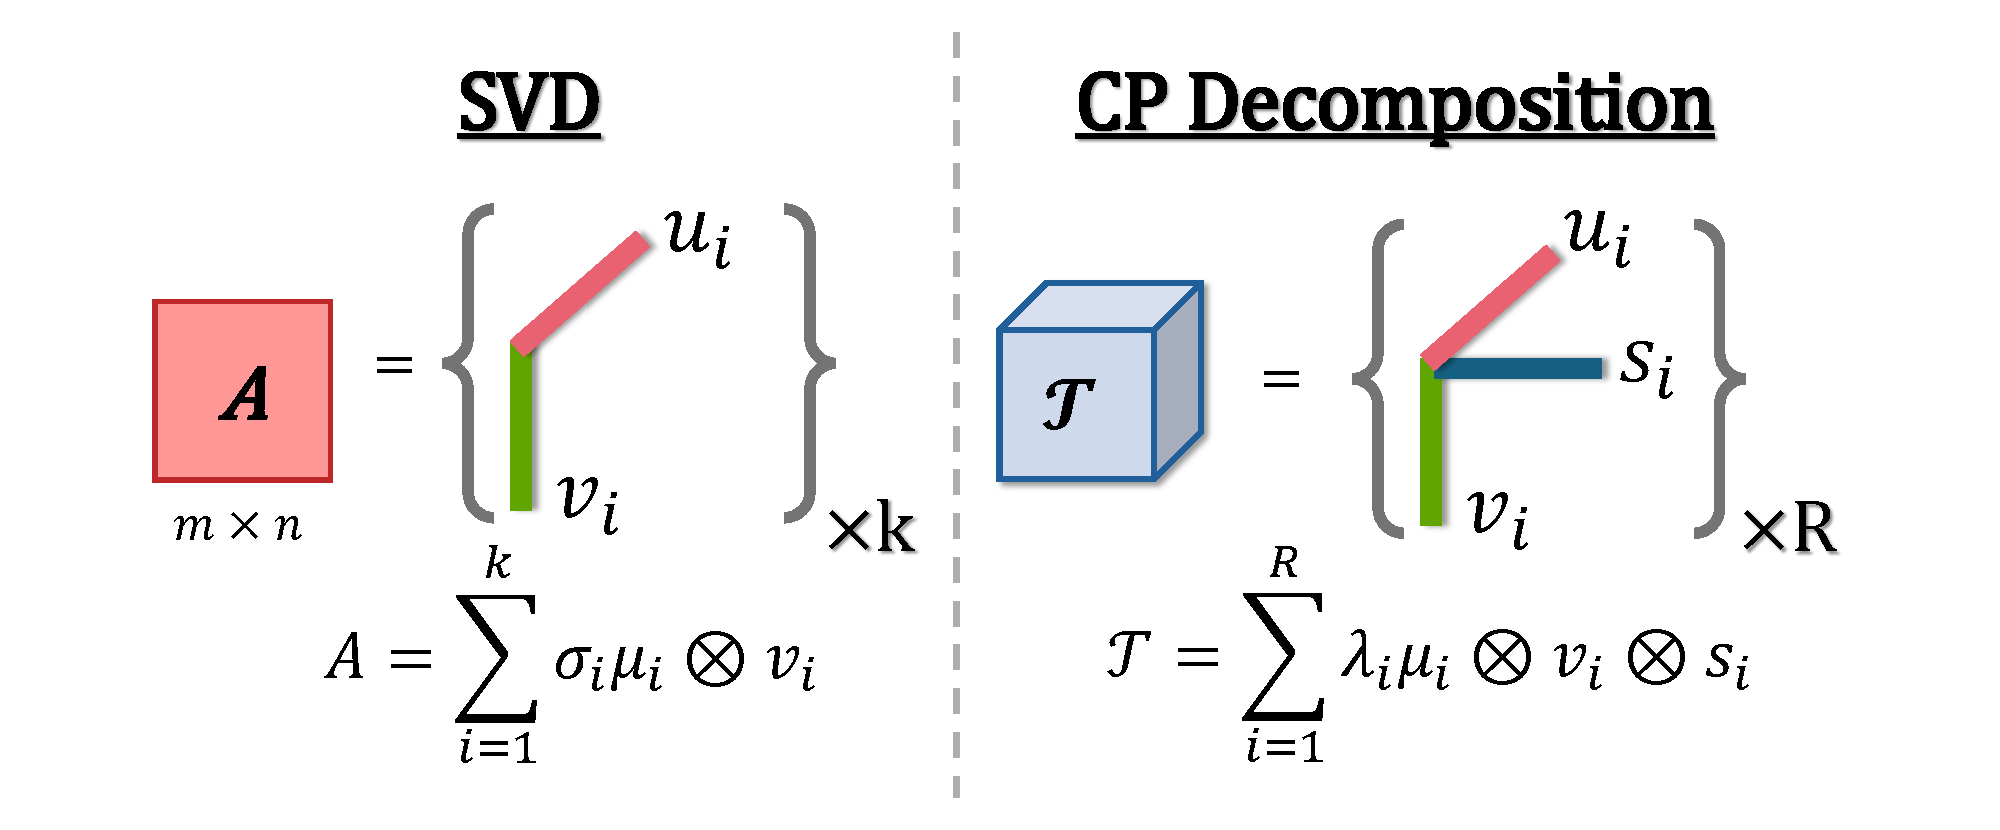
\includegraphics[width=\linewidth]{fig/CP.pdf}
        \caption{An illustration of SVD decomposition of a matrix
        $A\in\mathbb{R}^{m\times n}$ and CP decomposition of third-order tensor
        $\mathcal{T}$.}
        \label{fig:svd_cp}
    \end{wrapfigure}

    We model the interaction between LoRA adapters with tensor decomposition, which approximates a tensor by a set of low-rank factors. We use the Canonical Polyadic Decomposition (CPD), introduced by \citet{hitchcock1927expression,hitchcock1928multiple}, which represents a tensor as a sum of a minimal number of rank-one tensors (Fig.~\ref{fig:svd_cp}). CPD is a special case of the Tucker decomposition \citep{de2000multilinear,tucker1966some}, which multiplies a core tensor by a factor matrix along each mode. Tucker decomposition is more flexible, but its factors are not unique. We use CPD because, under mild conditions, its rank-one components are unique up to scaling and permutation, so the task-mode factors identify how each task contributes to each component. Given a third-order tensor $\mathcal{T}\in\mathbb{R}
    ^{I_1\times I_2\times I_3}$, the CP decomposition of rank $R$ is
    \begin{equation}
        \label{eq:cp_general}\mathcal{T}=\sum_{i=1}^{R}\lambda_{i}\mathbf{u}
        _{i}\otimes \mathbf{v}_{i}\otimes \mathbf{s}_{i},
    \end{equation}
    where $\lambda_{i}$ is the weight of the $i$-th component,
    $\mathbf{u}_{i}$, $\mathbf{v}_{i}$, and $\mathbf{s}_{i}$ are the factor vectors
    of the three modes of $\mathcal{T}$, and $\otimes$ denotes the outer product.


\section{Method}
 \begin{figure*}[htpb]
        \small
        \centering
        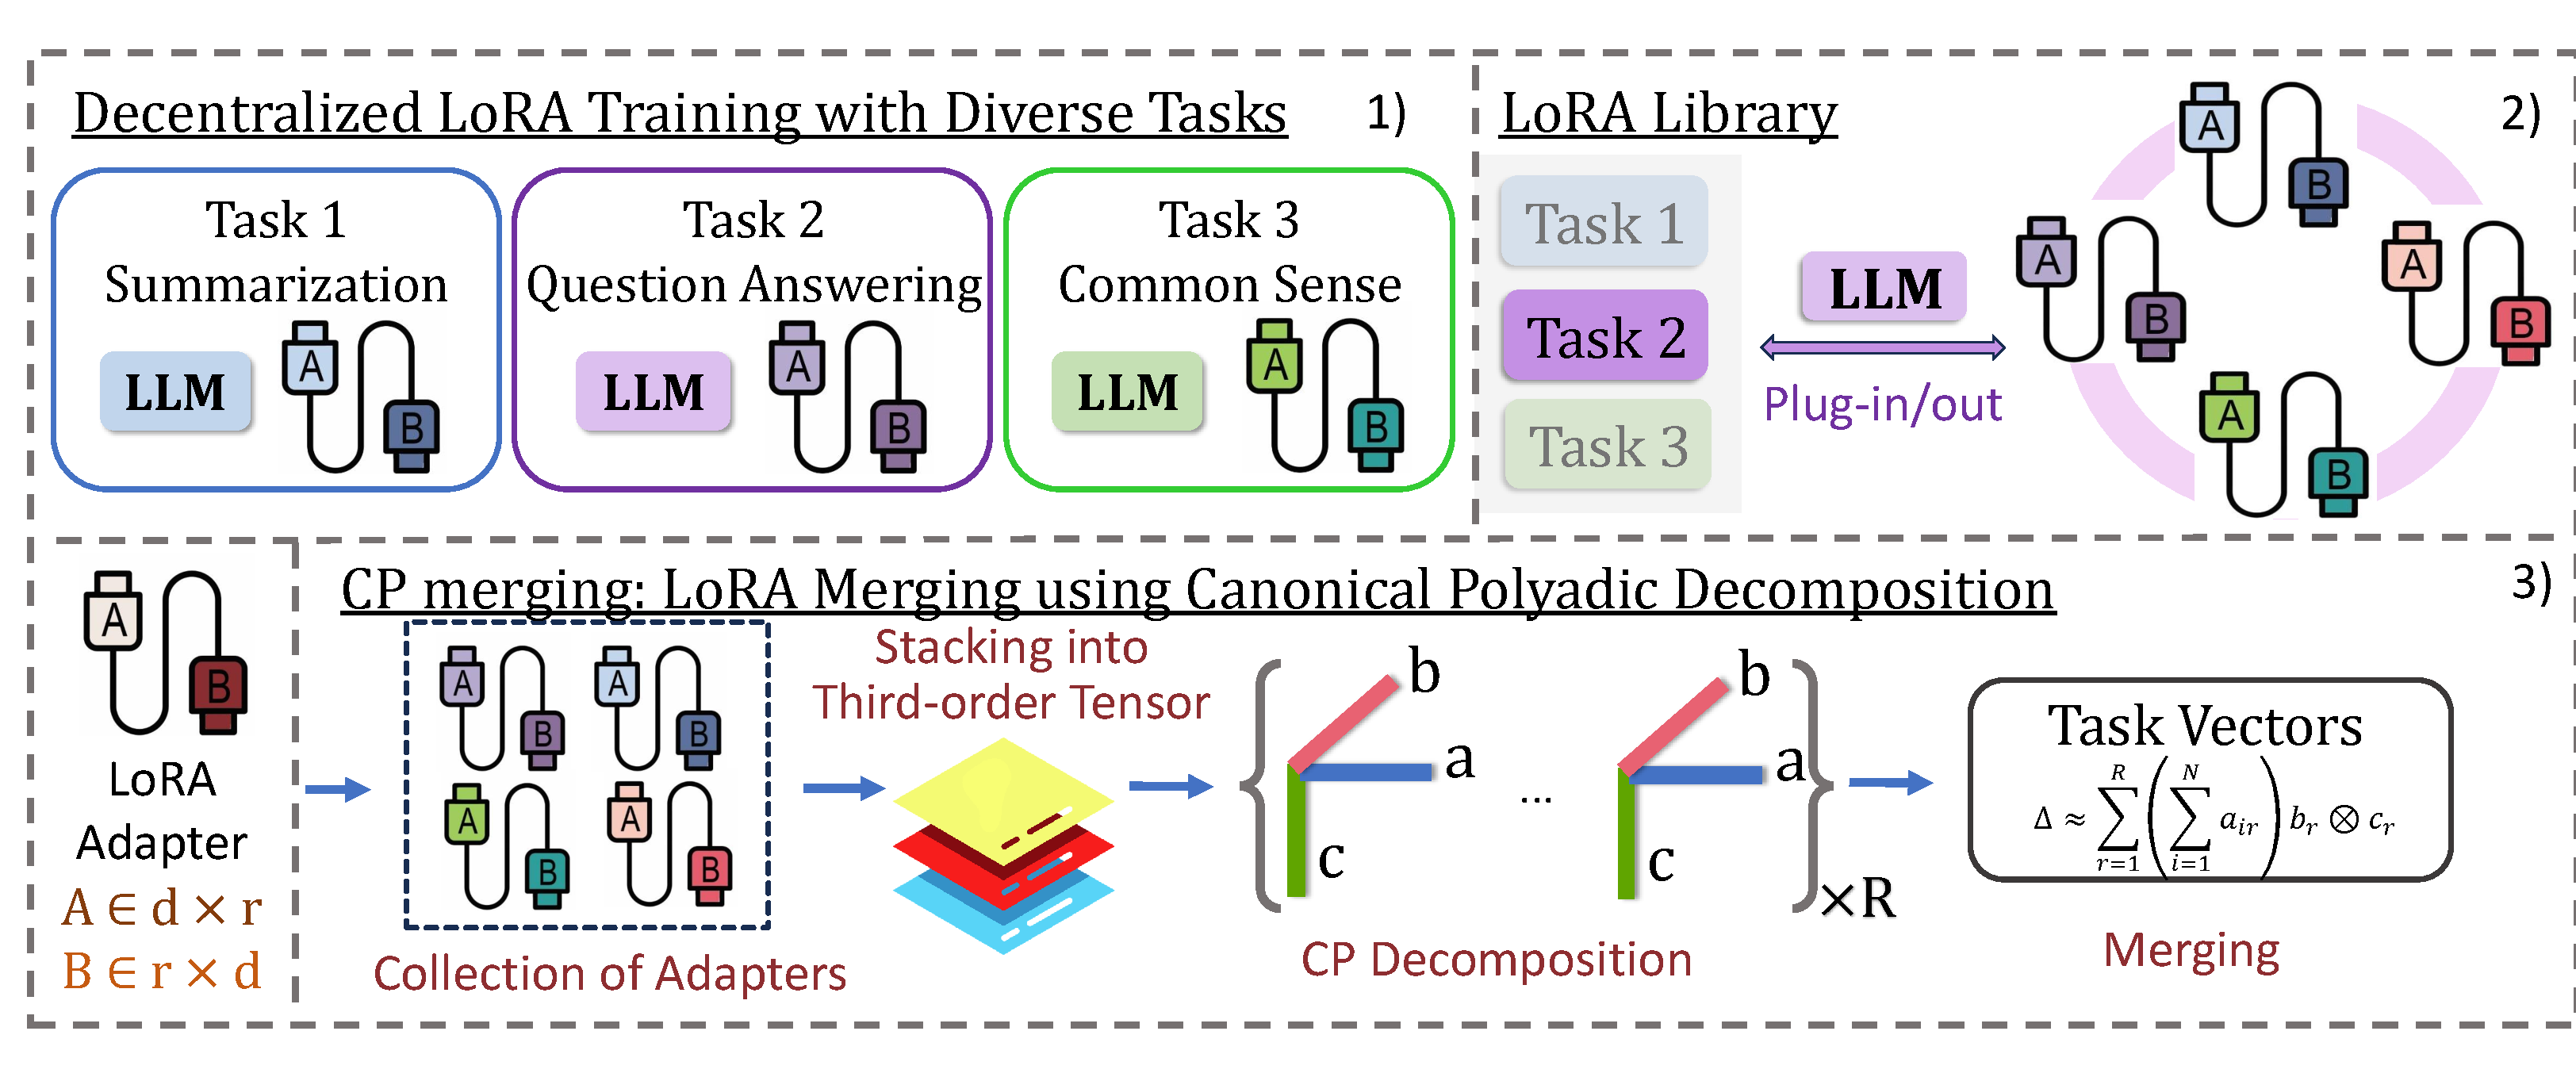
\includegraphics[width=0.99\linewidth]{fig/CP_merging.pdf}
        \caption{Overview of CP merging. (1) A LoRA adapter is trained
        independently for each task. (2) The adapters form a LoRA library whose
        modules can be added to or removed from the LLM. (3) CP merging stacks
        the adapters of a layer into a third-order tensor, factorizes it with CP
        decomposition, and merges the adapters over the task mode.}
        \label{fig:factorizing_lib}
    \end{figure*}
    \subsection{CP Merging}
    \paragraph{Task Singular Vectors}
    \citet{gargiulo2025task} decompose each layer-wise task matrix with SVD and
    call the resulting singular vectors \textit{task singular vectors} (TSVs).
    TSVs expose the low-rank structure of each task matrix and make the
    interaction between tasks measurable. For two tasks $i$ and $j$, the task
    matrices $\Delta_{i}$ and $\Delta_{j}$ are decomposed as

    \begin{align}
        \Delta_{i} & = U_{i}\Sigma_{i}V_{i}^{\top}, \quad \Delta_{j}= U_{j}\Sigma_{j}V_{j}^{\top}
    \end{align}

    where $U_{i}$ and $U_{j}$ contain the left singular vectors, $V_{i}$ and $V_{j}$
    contain the right singular vectors, and $\Sigma_{i}$ and $\Sigma_{j}$ are diagonal
    matrices of singular values. As shown in Fig.~\ref{fig:svd_cp}, SVD expresses a
    matrix as a sum of rank-one matrices. Keeping the top-$k$ singular values and
    their vectors gives the best rank-$k$ approximation of each task matrix:

    \begin{equation}
        \hat{\Delta}_{i}= \sum_{j=1}^{k}\sigma_{j}^{i}\, \mathbf{u}_{j}^{i}\otimes
        {\mathbf{v}_j^i}.
    \end{equation}
    \begin{wrapfigure}[18]{r}{0.50\textwidth}
\vspace{-20pt} 
  \centering
  \begin{minipage}{0.48\textwidth}
    \begin{algorithm}[H]
        \caption{Implementation of CP Merging}
        \algsetup{linenosize=\small} % Adjust line number size
        \begin{algorithmic}[1] % The [1] here means line numbers will be shown starting from 1
            \STATE Input: Pretrained task LoRA adapters$\{\Delta_{1},\Delta_{2},..., \Delta_{N}\}$, scaling factors $\alpha$. 
            \STATE \textbf{Output:
            Merged weight $W_{\mathrm{MT}}$} 
            
            % \STATE $E=[]$ 

            % \FOR{$i = 1$ to $N$} \STATE $\Delta_{i}$=Train($\mathcal{C}_{i}$, LLM)
            % \ENDFOR

            \STATE \textbf{Concatenate} the matrices: \STATE $\mathcal{T}\leftarrow
            [\Delta_{1}|\Delta_{2}|...|\Delta_{N}]$

            \STATE \textbf{CP Decomposition:}

            \STATE
            $\mathcal{T}\approx \sum_{r=1}^{R}\mathbf{a}_{r}\otimes \mathbf{b}_{r}
            \otimes \mathbf{c}_{r}$
            (Eq. \ref{eq:cp_decomposition})

            \STATE \textbf{Compute the Task Matrix:}

            \STATE
            $\Delta_{i}\approx \sum_{r=1}^{R}a_{ir}\textbf{b}_{r}\otimes \textbf{
             c}_{r}$
            \quad\quad (Eq.\ref{eq:cp_form})

            \STATE \textbf{Reconstruct} the merged matrix:

            \STATE $\Delta \approx \sum_{r=1}^{R}\left( \sum_{i=1}^{N}a_{ir}\right
            ) \textbf{b}_{r}\otimes \textbf{c}_{r}$ \quad (Eq.
            \ref{eq:cp_merge})

            \STATE \textbf{Construct} the merged model weights: \STATE
            $W_{\mathrm{merged}}=W_{\text{base}}+\alpha\sum_{r=1}^{R}\left( \sum_{i=1}^{N}a_{ir}\right
            ) \textbf{b}_{r}\otimes \textbf{c}_{r}$
            \STATE \textbf{return} $W_{\mathrm{MT}}$
        \end{algorithmic}
        \label{al:factorizing}
    \end{algorithm}
\end{minipage}
\end{wrapfigure}
    where $\hat{\Delta}_{i}$ is the rank-$k$ approximation of $\Delta_{i}$, and
    $\sigma_{j}^{i}$, $\mathbf{u}_{j}^{i}$, and $\mathbf{v}_{j}^{i}$ are its $j$-th
    singular value, left singular vector, and right singular vector.
    \texttt{Knots} computes an SVD $U\Sigma[V_1,V_2,\ldots,V_N]^{\top}$ of the concatenated task updates, merges the task-specific blocks $V_i$ into $V^{(\text{merged})}$, and reconstructs the merged update as $\Delta W^{(\text{merged})} = U\Sigma[V^{(\text{merged})}]^{\top}$. \texttt{TSV merging} decomposes each adapter separately and concatenates the left singular matrices $[U_1,U_2,\ldots,U_N]$ and right singular matrices $[V_1,V_2,\ldots,V_N]$. In TSV merging, the singular vectors of each task are therefore chosen without reference to the other tasks. CP merging instead decomposes all adapters jointly by treating them as one tensor.

    \paragraph{Representing all adapters as a Third-Order Tensor}
    
    We treat the task matrices $\Delta_{i}$ as slices of a third-order tensor
    $\mathcal{T}\in\mathbb{R}^{d_{in}\times d_{out}\times N}$, whose modes
    correspond to the input dimension, the output dimension, and the $N$ tasks.
    Each $\Delta_{i}\in\mathbb{R}^{d_{in}\times d_{out}}$ is the $i$-th frontal
    slice of $\mathcal{T}$, so $\mathcal{T}$ is obtained by stacking the
    $\Delta_{i}$ along the task mode.

    \paragraph{CP Decomposition Form}

    CP decomposition approximates $\mathcal{T}$ by a sum of $R$ rank-one tensors:

    \begin{equation}
        \label{eq:cp_decomposition}\mathcal{T}\approx \sum_{r=1}^{R}\lambda_r\,\mathbf{b}_{r}
        \otimes \mathbf{c}_{r}\otimes \mathbf{a}_{r},
    \end{equation}

    where the rank $R$ plays the role of $k$ in SVD, $\mathbf{a}_{r}
    \in \mathbb{R}^{N}$ is the task-mode factor, and
    $\mathbf{b}_{r}\in \mathbb{R}^{d_{in}}$ and
    $\mathbf{c}_{r}\in \mathbb{R}^{d_{out}}$ are the input-mode and output-mode
    factors. We absorb the weights into the factors and set $\lambda_r=1$. The
    $i$-th slice of $\mathcal{T}$ is then approximated as

    \begin{equation}
        \label{eq:cp_form}
        \Delta_{i}\approx \sum_{r=1}^{R}a_{ir}\mathbf{b}_{r}\otimes
        \mathbf{c}_{r}
    \end{equation}

    where $a_{ir}$, the $i$-th entry of $\mathbf{a}_{r}$, is the contribution of
    the $r$-th component to task $i$. All tasks share the rank-one matrices
    $\mathbf{b}_{r}\otimes\mathbf{c}_{r}$ and differ only in the coefficients
    $a_{ir}$. A component with large coefficients for many tasks represents
    shared structure, and a component whose coefficients are concentrated on one
    task represents task-specific structure.

    \paragraph{CP merging over the task mode}

    We merge the adapters by summing the slices over the task mode:

    \begin{equation}
        \Delta = \sum_{i=1}^{N}\Delta_{i}\approx \sum_{i=1}^{N}\sum_{r=1}^{R}a_{ir}
        \mathbf{b}_{r}\otimes \mathbf{c}_{r}
    \end{equation}

    Because $\mathbf{b}_{r}\otimes \mathbf{c}_{r}$ does not depend on $i$, the
    sum factorizes as
    \begin{equation}
        \label{eq:cp_merge}\Delta \approx \sum_{r=1}^{R}\left( \sum_{i=1}^{N}a_{ir}
        \right) \mathbf{b}_{r}\otimes \mathbf{c}_{r}
    \end{equation}

    where $\sum_{i=1}^{N}a_{ir}$ is the total contribution of the $r$-th component
    across tasks. The merged weights are

    \begin{equation}
        W_{\text{merged}}=W_{\text{base}}+\alpha\sum_{r=1}^{R}\left( \sum_{i=1}^{N}a_{ir}\right) \mathbf
        {b}_{r}\otimes \mathbf{c}_{r}.
    \end{equation}

    Algorithm~\ref{al:factorizing} summarizes the procedure, which is applied independently to every adapted layer.

\section{Experimental Results}

    We compare CP merging with existing LoRA merging methods on held-in and held-out Flan tasks (Sec.~\ref{sec:held_in_out}) \citep{arnobexploring,ostapenko2024towards}, on zero-shot benchmarks (Sec.~\ref{sec:zero_shot}) \citep{ostapenko2024towards}, and on skill composition (Appendix~\ref{sec:skill_composition}) \citep{prabhakar2025lora}.

    \paragraph{Baselines}
    We use the following baselines in all settings unless stated otherwise. \textbf{BASE}: the
    pre-trained model without adaptation. \textbf{Multi-task}: a single LoRA
    adapter fine-tuned on the union of the training sets. \textbf{Uniform}:
    one LoRA adapter per task, averaged uniformly
    \citep{huang2023lorahub,chronopoulou2023adaptersoup}. \textbf{Task
    Arithmetic (TA)} \citep{ilharco2022editing}: task vectors, defined as the
    difference between fine-tuned and pre-trained weights, are summed linearly.
    \textbf{Ties-merging} \citep{yadav2023ties}: low-magnitude weights are pruned,
    and only weights that agree with the dominant sign are averaged. \textbf{DARE}
    \citep{yu2024language}: fine-tuned weights are randomly dropped and the
    remaining ones rescaled to obtain sparse task vectors; we combine it with
    TA and Ties. \textbf{TSV merging} \citep{gargiulo2025task}: each task matrix
    is compressed with SVD, and task singular vectors are decorrelated before
    merging. \textbf{Knots} \citep{stoica2025model}: a joint SVD maps the LoRA
    updates into a shared space before merging. \textbf{ISO-C}
    \citep{marczak2025no}: the singular value spectrum of the merged task
    matrix is flattened to an isotropic one.
    \begin{table*}[h]
\small
\centering
\begin{adjustbox}
{width=1.0\textwidth}
\begin{tabular}{l|ccccccccccc|c} 
\Xhline{1.6pt}
\textbf{Model} & \textbf{Wiqa} & \textbf{Sciq} & \textbf{Adver} & \textbf{Duorc} & \textbf{Cos} & \textbf{Wikiqa} & \textbf{Quail} & \textbf{Wikihop} & \textbf{ParaphQa} & \textbf{Yelp} & \multicolumn{1}{c}{\textbf{AVG}} & \textbf{3 Held-Out} \\
\midrule

\rowcolor{lightgray}\multicolumn{13}{c}{\textbf{Phi-3 (3B) with LoRA library }} \\
\textbf{BASE} & 14.55 & 7.99 & 10.85 & 7.32 & 5.00 & 4.17 & 11.88 & 3.51 & 6.93 & 8.33 & \cellcolor[HTML]{FDE9E8} 8.05 & \cellcolor[HTML]{FDE9E8}  16.00 \\ 
\textbf{Oracle} & 36.87 & 79.56 & 51.58 & 52.40 & 42.99 & 55.94 & 51.51 & 46.58 & 8.325 & 32.71 & \cellcolor[HTML]{FDE9E8}45.85 & \cellcolor[HTML]{FDE9E8}- \\
% \textbf{Multi-task}   & &\cellcolor[HTML]{FDE9E8} & \\

\midrule
\textbf{Uniform} & 22.98 & 61.97 & 29.61 & 18.45 & 28.12 & 11.56 & 38.94 & 7.194  & 7.18 & 15.66  & \cellcolor[HTML]{FDE9E8}24.17 & \cellcolor[HTML]{FDE9E8}\textbf{61.13}\\

\textbf{Ties-merging} & 23.33 & 51.52 & 30.15 & 18.05 & 30.12 & 12.54 & 35.05 & 10.03 & 5.80 & 16.76 & \cellcolor[HTML]{FDE9E8}23.34 & \cellcolor[HTML]{FDE9E8}34.69\\

\textbf{Ties w/DARE} & 25.42 & 52.76 & 32.34 & 19.04 & 31.20 & 13.33 & 36.05 & 7.05 & 6.08 & 16.00 & \cellcolor[HTML]{FDE9E8}23.93 & \cellcolor[HTML]{FDE9E8}34.70\\

\textbf{ISO-C} & 14.59 & 8.19 & 11.11 & 7.50 & 5.38 & 4.20 & 12.23 & 3.53 & 6.95 & 8.39 & \cellcolor[HTML]{FDE9E8}8.20 & \cellcolor[HTML]{FDE9E8}16.18\\
\textbf{TSV Merging} & 36.75 & 53.52 & 44.39 & 20.20 & 59.13 & 23.20& 37.25 & 34.70 & 4.78 & 34.95 & \cellcolor[HTML]{FDE9E8}34.89 & \cellcolor[HTML]{FDE9E8}45.70\\
\textbf{Knots} & 26.33 & 90.81 & 40.15 & 28.87 & 50.44 & 48.35 & 43.24 & 13.71 & 6.63 & 23.56 & \cellcolor[HTML]{FDE9E8}\underline{37.21} & \cellcolor[HTML]{FDE9E8}54.46\\

\midrule

\textbf{CP Merging} & 34.69 & 89.88 & 44.32 & 31.59 & 66.82 & 50.34 & 45.49 & 10.73 & 5.90 & 24.23 & \cellcolor[HTML]{FDE9E8}\textbf{40.40} & \cellcolor[HTML]{FDE9E8}\underline{60.15} \\

\midrule

\Xhline{1.6pt}
\end{tabular}
\end{adjustbox}
\caption{10 held-in and 3 held-out Flan tasks based on Phi-3 3B model. We report the Rouge-L scores. The oracle here denotes that we use the trained LoRA to test the corresponding tasks, which achieve the best results for held-in results. The task details are presented in Appendix \ref{sec:10_held_in}. }
\label{tab:in_domain_full}
\end{table*}
    \subsection{Held-In and Held-out Multi-Tasks}
    \label{sec:held_in_out}

    We use the Flan collection \citep{longpre2023flan} and
    sample 10 held-in and 3 held-out tasks following \citet{ostapenko2024towards} and \citet{arnobexploring}.
    Each task is sub-sampled to 10,000 examples, of which 1,000 are used for
    validation and early stopping.

   
    \begin{wrapfigure}[18]{r}{0.5\textwidth}
    \vspace{-15pt} 
        \small
        \centering
        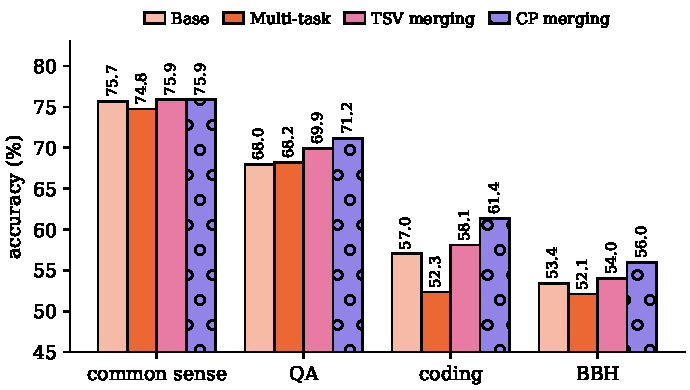
\includegraphics[width=0.50\textwidth]{fig/zero_shot_category.pdf}
        \caption{Zero-shot accuracy on Phi-3 per task category, averaged from Table~\ref{tab:zeroshot_full}. CP merging uses the C-LoRA library; the other methods use the standard library.}
        \label{fig:performance_categories}
    \end{wrapfigure}
    Table~\ref{tab:in_domain_full} reports Rouge-L on the 10 held-in tasks and the 3 held-out tasks. The Oracle row evaluates each task with its own LoRA adapter and serves as an upper bound for the held-in tasks (45.85). Among merging methods, CP merging obtains the highest held-in average (40.40), 3.19 points above Knots (37.21), the strongest SVD-based baseline, and 5.51 points above TSV merging (34.89). On the held-out tasks, CP merging reaches 60.15, compared with 54.46 for Knots and 45.70 for TSV merging. Uniform merging obtains the best held-out score (61.13) but a much lower held-in average (24.17), so averaging preserves general ability while losing most of the task-specific gains. Ties-merging and Ties w/DARE reach held-in averages of 23.34 and 23.93, close to uniform merging. ISO-C stays near the base model on both splits (8.20 and 16.18).

    \subsection{Zero-shot Experiments}
    \label{sec:zero_shot}
    \begin{table*}[ht]
\small
\centering
\begin{adjustbox}
{width=1.0\textwidth}
\begin{tabular}{l|cccccccccc|c} 
\Xhline{1.6pt}
\multicolumn{1}{c|}{} & \multicolumn{3}{c}{\textbf{Common Sense}} & \multicolumn{4}{c}{\textbf{Question Answering}} & \multicolumn{2}{c}{\textbf{Coding}} & \multicolumn{1}{c}{\textbf{ Reasoning}} & \multicolumn{1}{c}{\textbf{AVG}} \\
\cmidrule(lr){2-4}  \cmidrule(lr){5-8} \cmidrule(lr){9-10}
\cmidrule(lr){11-11}
\multicolumn{1}{c|}{} & \textbf{Piqa} & \textbf{Wg} & \textbf{Hswag} & \textbf{Boolq} & \textbf{Obqa} & \textbf{ArcE} & \textbf{ArcC} & \textbf{HE} & \textbf{Mbpp} & \textbf{BBH} & \multicolumn{1}{c}{\textbf{AVG}} \\
\midrule

\rowcolor{lightgray}\multicolumn{12}{c}{\textbf{Phi-3 (3B) with LoRA library }} \\
\textbf{BASE} & 81.1 & 70.2 & 75.7 & 85.0 & \textbf{49.0} & 80.0 & 57.9 & 53.0 & 61.1 & 53.4 & \cellcolor[HTML]{FDE9E8}66.6\\ 

\textbf{Multi-task}   & 79.1&69.6&75.6&87.1&47.6&82.6&55.6&51.8&52.9& 52.1 &\cellcolor[HTML]{FDE9E8}65.4 \\

\textbf{Uniform} & 81.0&70.4&76.0&84.7&48.8&82.4&57.9&52.4&63.0&55.6&\cellcolor[HTML]{FDE9E8}67.2\\

\textbf{Ties-merging} & 80.8 & \textbf{70.9} & 75.4 & 80.8 & 46.0 & 85.8 & 60.8 & 54.9 & 61.5 & 51.9 & \cellcolor[HTML]{FDE9E8}66.9 \\
\textbf{Task Arithmetic} & 81.0 & 70.5 & 75.9 & 84.7 & 48.8 & 82.5 & 58.2 & 54.3 & 61.9 & 54.2 & \cellcolor[HTML]{FDE9E8}67.2\\
\textbf{Ties w/DARE} & 80.7 & 70.8 & 75.2 & 82.8 & 46.3 & 84.8 & 60.9 & 54.9 & 61.6 & 52.0 & \cellcolor[HTML]{FDE9E8}67.0  \\
\textbf{TA w/DARE} & 81.2 & 70.1 & 75.3 & 84.9 & 48.9 & 82.2 & 58.3 & 54.5 & 61.1 & 54.3 & \cellcolor[HTML]{FDE9E8}67.1 \\
\textbf{TSV Merging} & 81.1 & 70.8 & 75.8 & 86.0 & \textbf{49.0} & 84.3 & 60.4 & 55.0 & 61.2 & 54.0 & 67.7\cellcolor[HTML]{FDE9E8}\\
\midrule
\rowcolor{lightgray}\multicolumn{12}{c}{\textbf{Phi-3 (3B) with C-LoRA library }} \\
\textbf{Uniform} & 81.5 & 69.5 & 76.0 & 86.6 & 48.8 & 86.7  & 61.8 & 57.3  & 65.3 & 55.9  & \cellcolor[HTML]{FDE9E8}\underline{68.9} \\
\textbf{Knots} & 80.8 & 71.7 & 74.9 & 85.0 & 48.0 & 84.1 & 58.2 & 53.2 & 62.6 & 50.4 & \cellcolor[HTML]{FDE9E8}66.9 \\
\textbf{TSV Merging} & 81.3 & 69.3 & 75.6 & 86.4 & 48.8 & 86.1 & 62.3 & 52.4 & 63.3 & 55.1 & \cellcolor[HTML]{FDE9E8}68.1\\
% \textbf{Core merging} \\
\textbf{CP merging} & \textbf{81.7} & 70.0 & \textbf{76.0} & \textbf{86.6}  & 48.9 & \textbf{86.7} & \textbf{62.5}& \textbf{57.3}  & \textbf{65.4} & \textbf{56.0}  & \cellcolor[HTML]{FDE9E8}\textbf{69.1}  \\

\midrule


\Xhline{1.6pt}
\end{tabular}
\end{adjustbox}
\caption{Zero-shot accuracy on 10 downstream benchmarks with Phi-3 (\texttt{microsoft/Phi-3-mini-4k-instruct}). C-LoRA is a LoRA library built by clustering instruction embeddings (Appendix~\ref{sec:clora}). Results with Mistral-7B are in Appendix~\ref{sec:zero_shot_mistral}, and the experimental setting is in Appendix~\ref{sec:exp_setting}.}
\label{tab:zeroshot_full}
\end{table*}

    To measure out-of-domain generalization, we evaluate the merged models on
    zero-shot benchmarks from four categories: \textbf{common-sense reasoning}
    (WinoGrande \citep{sakaguchi2021winogrande}, HellaSwag \citep{zellers2019hellaswag},
    and PIQA \citep{bisk2020piqa}), \textbf{question answering} (BoolQ \citep{clark2019boolq},
    OpenBookQA \citep{mihaylov2018can}, ARC-Easy, and ARC-Challenge \citep{clark2018think}),
    \textbf{coding} (HumanEval \citep{chen2021evaluating} and MBPP \citep{austin2021program}),
    and \textbf{general-purpose reasoning} (BBH \citep{suzgun2023challenging}).
    Besides the standard library of 256 task adapters, we also merge a clustered
    library (C-LoRA, Appendix~\ref{sec:clora}), in which each adapter is trained
    on a cluster of similar instructions.

    \subsubsection{Experimental results}

    Table~\ref{tab:zeroshot_full} reports zero-shot accuracy on the 10 benchmarks
    with Phi-3. The multi-task adapter (65.4\%) underperforms the base model
    (66.6\%), which is consistent with \textit{catastrophic forgetting}, where
    newly learned parameters overwrite knowledge acquired during pre-training
    \citep{wang2024comprehensive}. Uniform merging of the 256-adapter library
    reaches 67.2\%.

    With the C-LoRA library, TSV merging (68.1\%) outperforms Knots (66.9\%),
    and CP merging obtains the highest average accuracy (69.1\%). CP merging is
    best or tied for best on 7 of the 10 benchmarks, and uniform merging of the same
    library is close behind (68.9\%). The exceptions are WinoGrande, where
    Knots is best (71.7\%), BoolQ, where the multi-task adapter is best (87.1\%),
    and OpenBookQA, where the base model and TSV merging with the standard
    library reach 49.0\%. Results on Mistral-7B, reported in
    Appendix~\ref{sec:zero_shot_mistral}, follow the same ordering, with CP
    merging reaching 65.0\% compared with 64.9\% for uniform merging and 62.7\%
    for TSV merging.

    Figure~\ref{fig:performance_categories} breaks the results down by category,
    averaging the accuracies in Table~\ref{tab:zeroshot_full}. Compared with TSV
    merging on the standard library, CP merging gains 3.3 points on coding, 2.0 on
    BBH, and 1.3 on question answering, and matches it on common-sense reasoning
    (75.9 for both). The effect of task interference therefore appears to depend
    on the task type.

\section{Analysis}

    % To investigate the reasons behind the observed improvements, we conducted further analysis.  As previously mentioned, the CP rank $R$ is a critical hyperparameter in CP decomposition. Analyzing $R$ allows us to identify the most impactful components, so we examine the influence of CP rank on performance (Sec. \ref{sec:rank_analyse}). Furthermore, we study the number of clustering approaches (Sec. \ref{sec:clustering}). We also study how CP merging can
    % reduce task interference in \textit{parameter-level} (Sec. \ref{sec:cp_merging}). Lastly, we analyze the memory requirements of different library approaches (Sec. \ref{sec:memory_usage}).

    % \begin{figure}[h]
    %     \centering
    %     \includegraphics[width=\linewidth]{fig/common-sense.png}
    %     \caption{Comparison of our approaches on Common-sense
    % reasoning tasks. We present all the results based on Phi-3.}
    %     \label{fig:common_sense_reasoning}
    % \end{figure}

    % \begin{figure}[h]
    %     \centering
    %     \includegraphics[width=\linewidth]{fig/coding.png}
    %     \caption{Comparison of our approaches on Coding
    % tasks. }
    %     \label{fig:coding}
    % \end{figure}

    


\subsection{Number of merged tasks}


Table~\ref{tab:tasks_size} varies the number of merged Flan tasks. All merging methods improve substantially over the base model, which scores 11.14, 9.15, and 8.05 Rouge-L for 3, 5, and 10 tasks. CP merging obtains the highest score at every size. With 3 tasks it matches Knots (59.06 vs.\ 59.04) and is far ahead of TSV merging (44.87). With 5 tasks, TSV merging and Knots both reach 54.4, while CP merging reaches 57.7. With 10 tasks, all methods drop, and CP merging remains the best (40.40, compared with 37.21 for Knots and 34.89 for TSV merging). The gap between CP merging and the best SVD-based method is negligible for 3 tasks and above 3 points once 5 or more adapters are merged.
\begin{table}[h]
    \centering
    \begin{tabular}{l|ccc}
    \toprule
      Model  & 3 tasks & 5 tasks & 10 tasks \\
    \midrule
     Base    & 11.14 & 9.15 & 8.05\\
     TSV merging & 44.87 & 54.4 & 34.89\\
     Knots & 59.04 & 54.4& 37.21\\
     \midrule
     CP merging & \textbf{59.06} & \textbf{57.7} & \textbf{40.40}\\
     \bottomrule
    \end{tabular}
    \caption{Effect of the number of merged tasks. We merge 3, 5, and 10 Flan tasks and report the average Rouge-L over the merged tasks.}
    \label{tab:tasks_size}
\end{table}



\subsection{CP Merging for Task Interference} 
\label{sec:cp_merging}


% \begin{wrapfigure}[13]{r}{0.5\textwidth}
% \vspace{-20pt}
% \centering
% 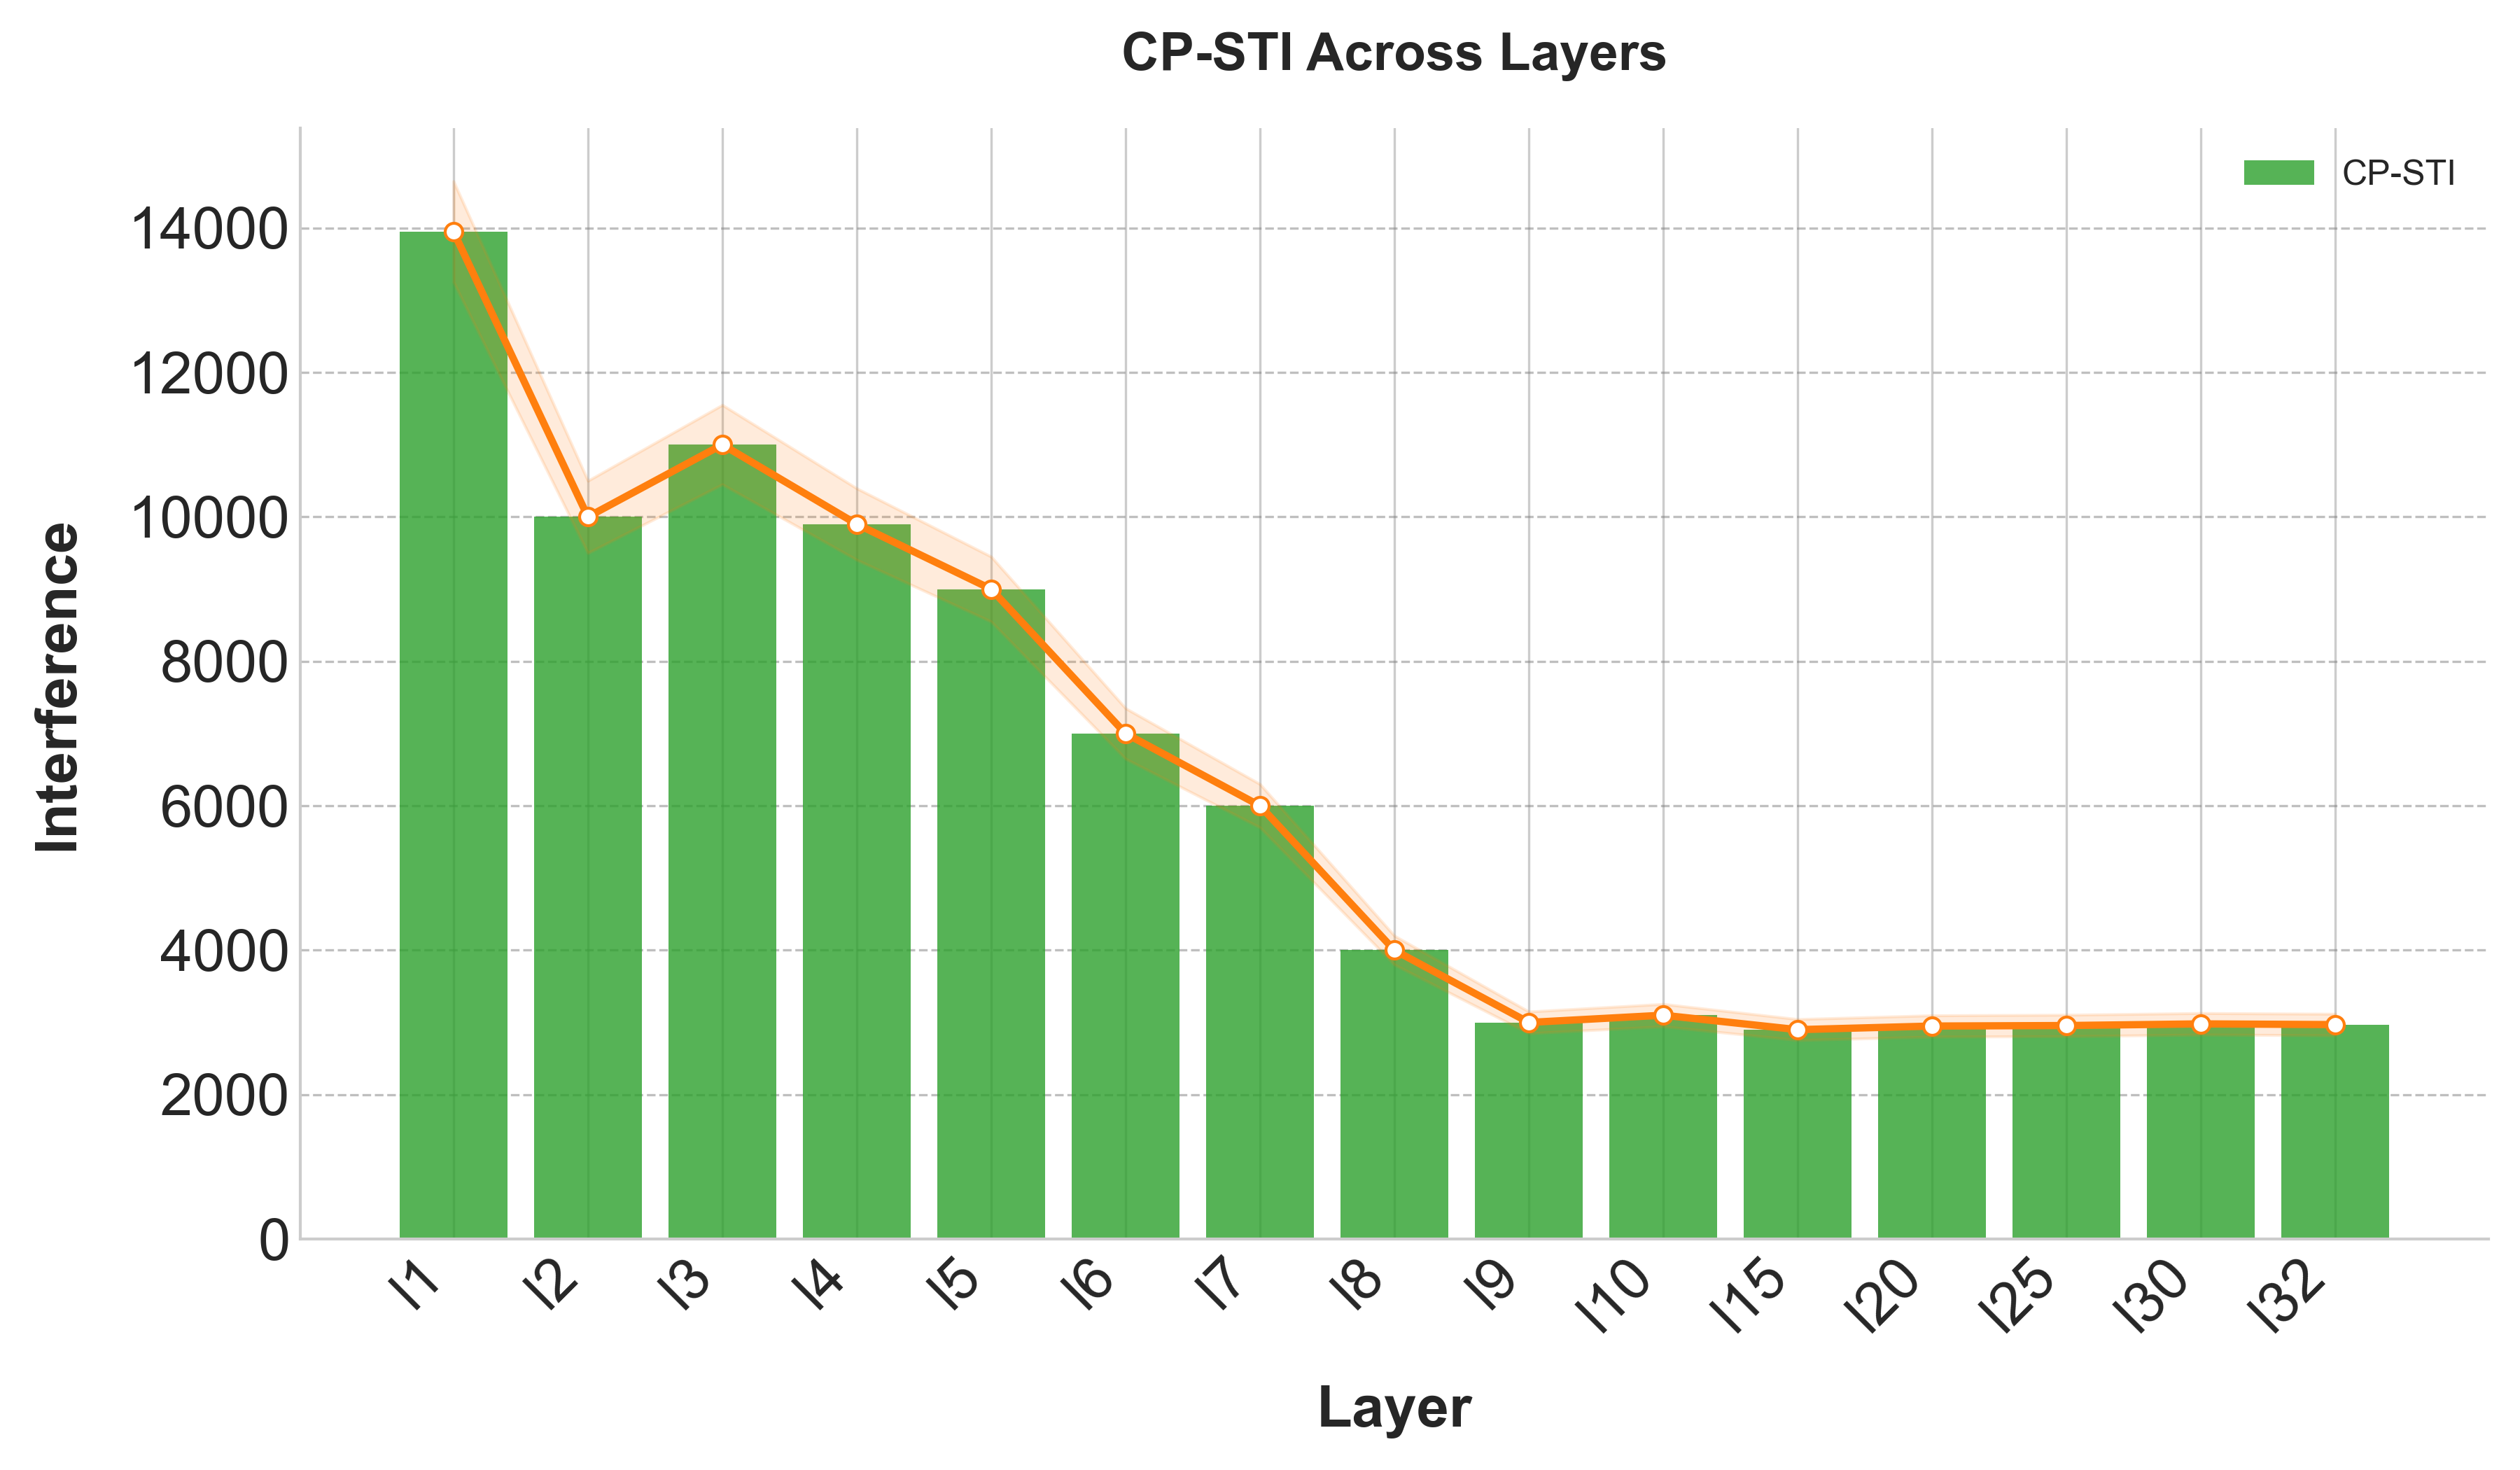
\includegraphics[width=0.5\textwidth]{fig/cp_sti_across_layers.png}
% \caption{CP-STI across layers in the LLama 7B for Math and Code LoRA.}
% \label{fig:cp_str_interference}
% \end{wrapfigure}

\citet{gargiulo2025task} measure task interference with the \textit{Singular Task Interference} (STI) score, which quantifies the overlap between the TSVs of different tasks:

\begin{equation}
    \textbf{STI}\left( \left\{ \Delta_i \right\}_{i=1}^{N} \right) 
= \left\| \left( U^\top U - I \right) \Sigma \left( V^\top V - I \right) \right\|_1
\end{equation}

Large off-diagonal inner products in $U^{\top}U$ and $V^{\top}V$ indicate that tasks share singular directions, and \citet{gargiulo2025task} associate such overlap with a higher likelihood of interference after merging. We extend this score to CP factors. Overlapping CP components play the same role as overlapping singular vectors, so we measure how far the factor matrices of all three modes deviate from orthogonality and define the CP-based Singular Task Interference (CP-STI) as
\begin{equation}
\label{eq:cp_sti}
  \textbf{CP-STI}(\{\Delta_i\}_{i=1}^N) = \|(A^{\top} A - I) \circ (B^{\top} B - I) \circ (C^{\top} C - I)\|_1,
\end{equation}




\begin{figure}[h]
    \centering
    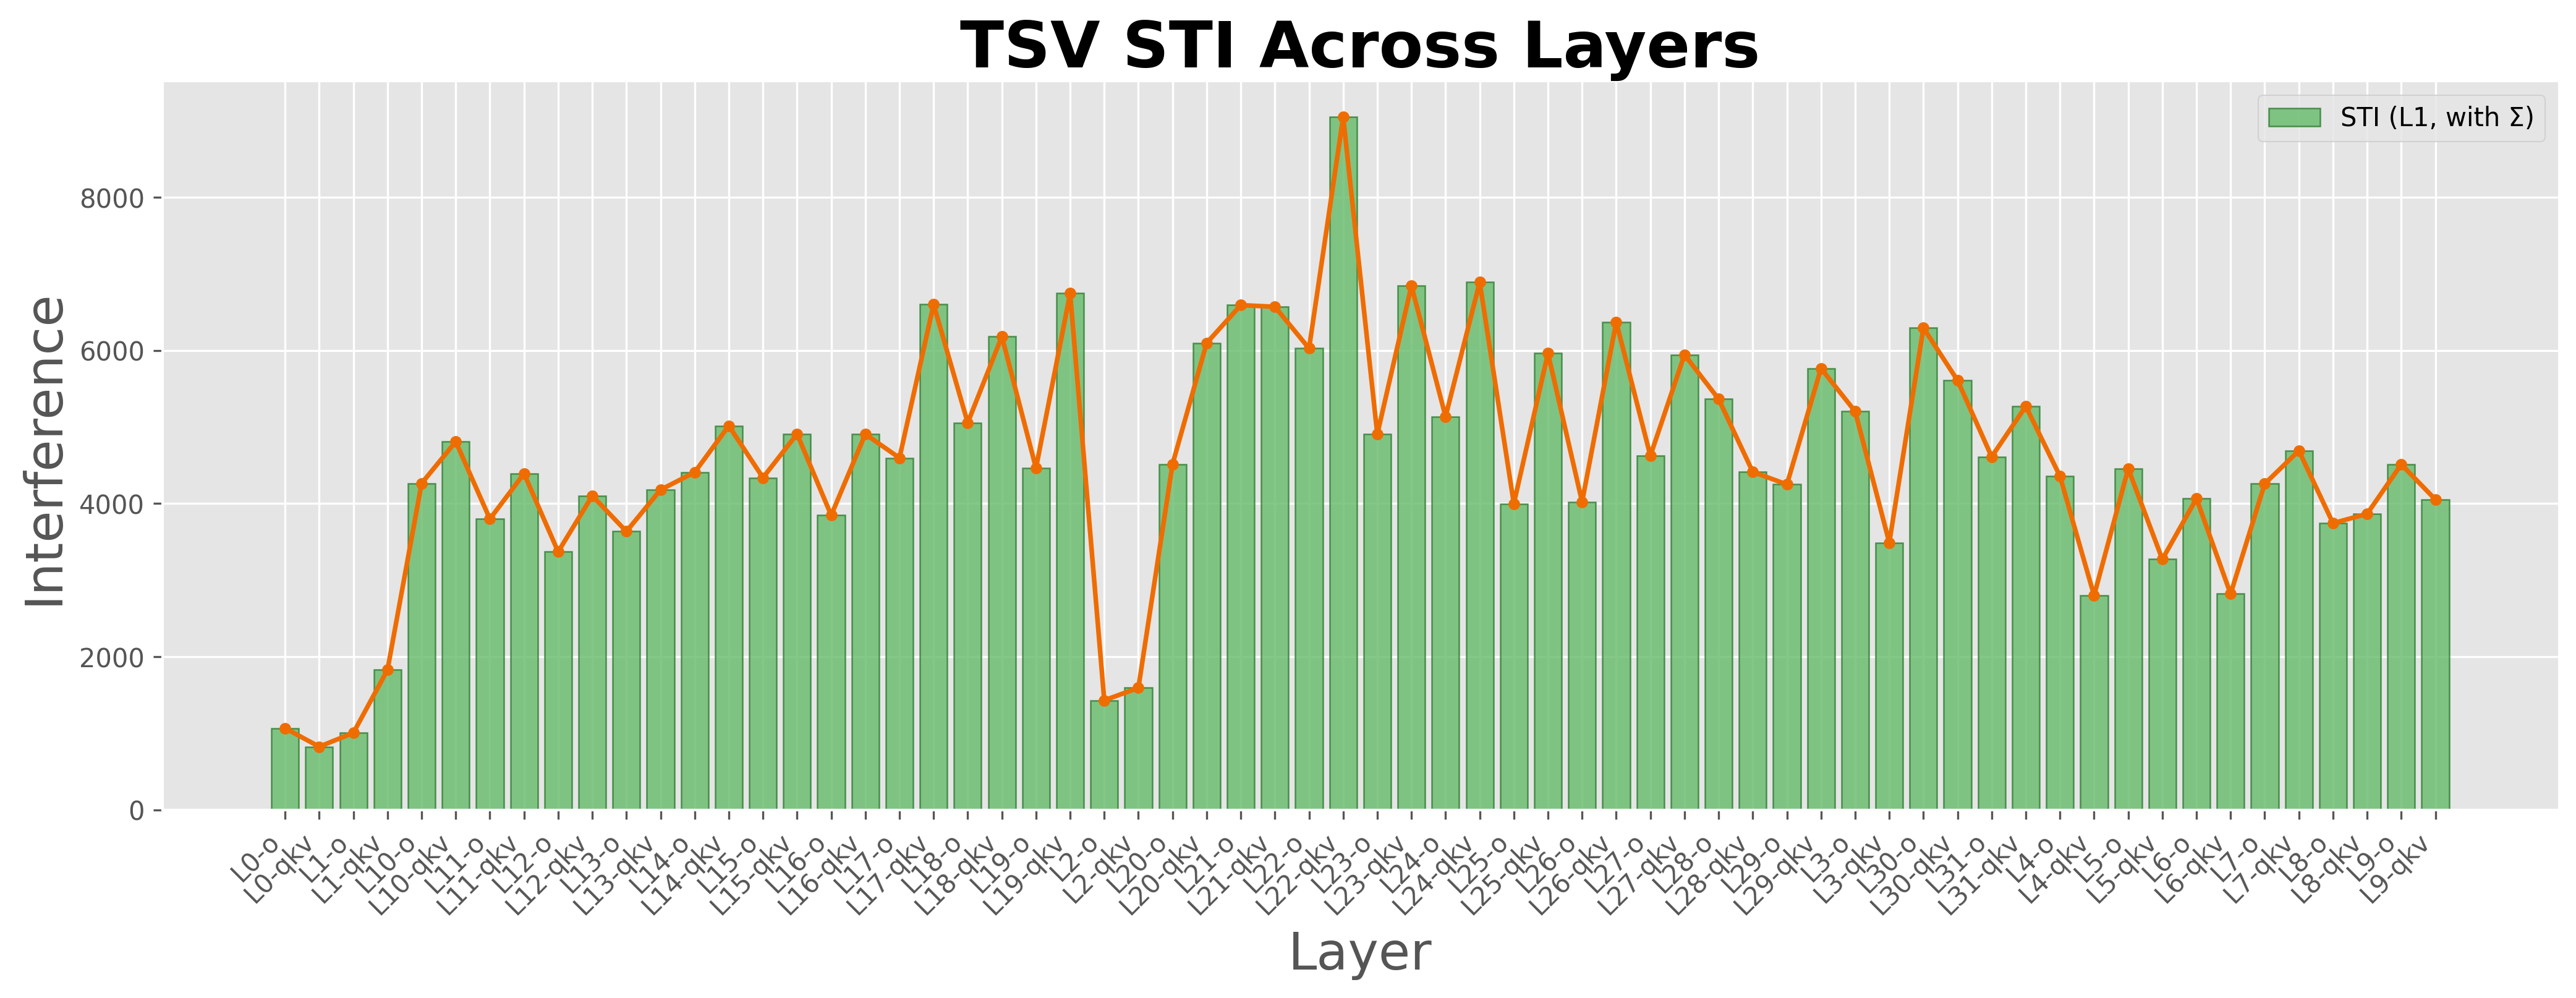
\includegraphics[width=0.7\linewidth]{fig/tsvmerge_sti_across_layers_beautified.png}
    \caption{STI of TSV merging across layers on 5 Flan tasks.}
    \label{fig:sti}
\end{figure}
where $A=[\mathbf{a}_1, \ldots, \mathbf{a}_R] \in \mathbb{R}^{N \times R}$, $B=[\mathbf{b}_1, \ldots, \mathbf{b}_R] \in \mathbb{R}^{d_{in} \times R}$, and $C= [\mathbf{c}_1, \ldots, \mathbf{c}_R] \in \mathbb{R}^{d_{out} \times R}$ stack the task-mode, input-mode, and output-mode factors, $\circ$ denotes the Hadamard product, and $I$ is the $R \times R$ identity matrix. A large CP-STI means that components overlap in all three modes at once, so their contributions are hard to separate after merging.




% \begin{figure}[h]
%         \centering
%         \begin{subfigure}
%             {0.45\textwidth}
%             \centering
%         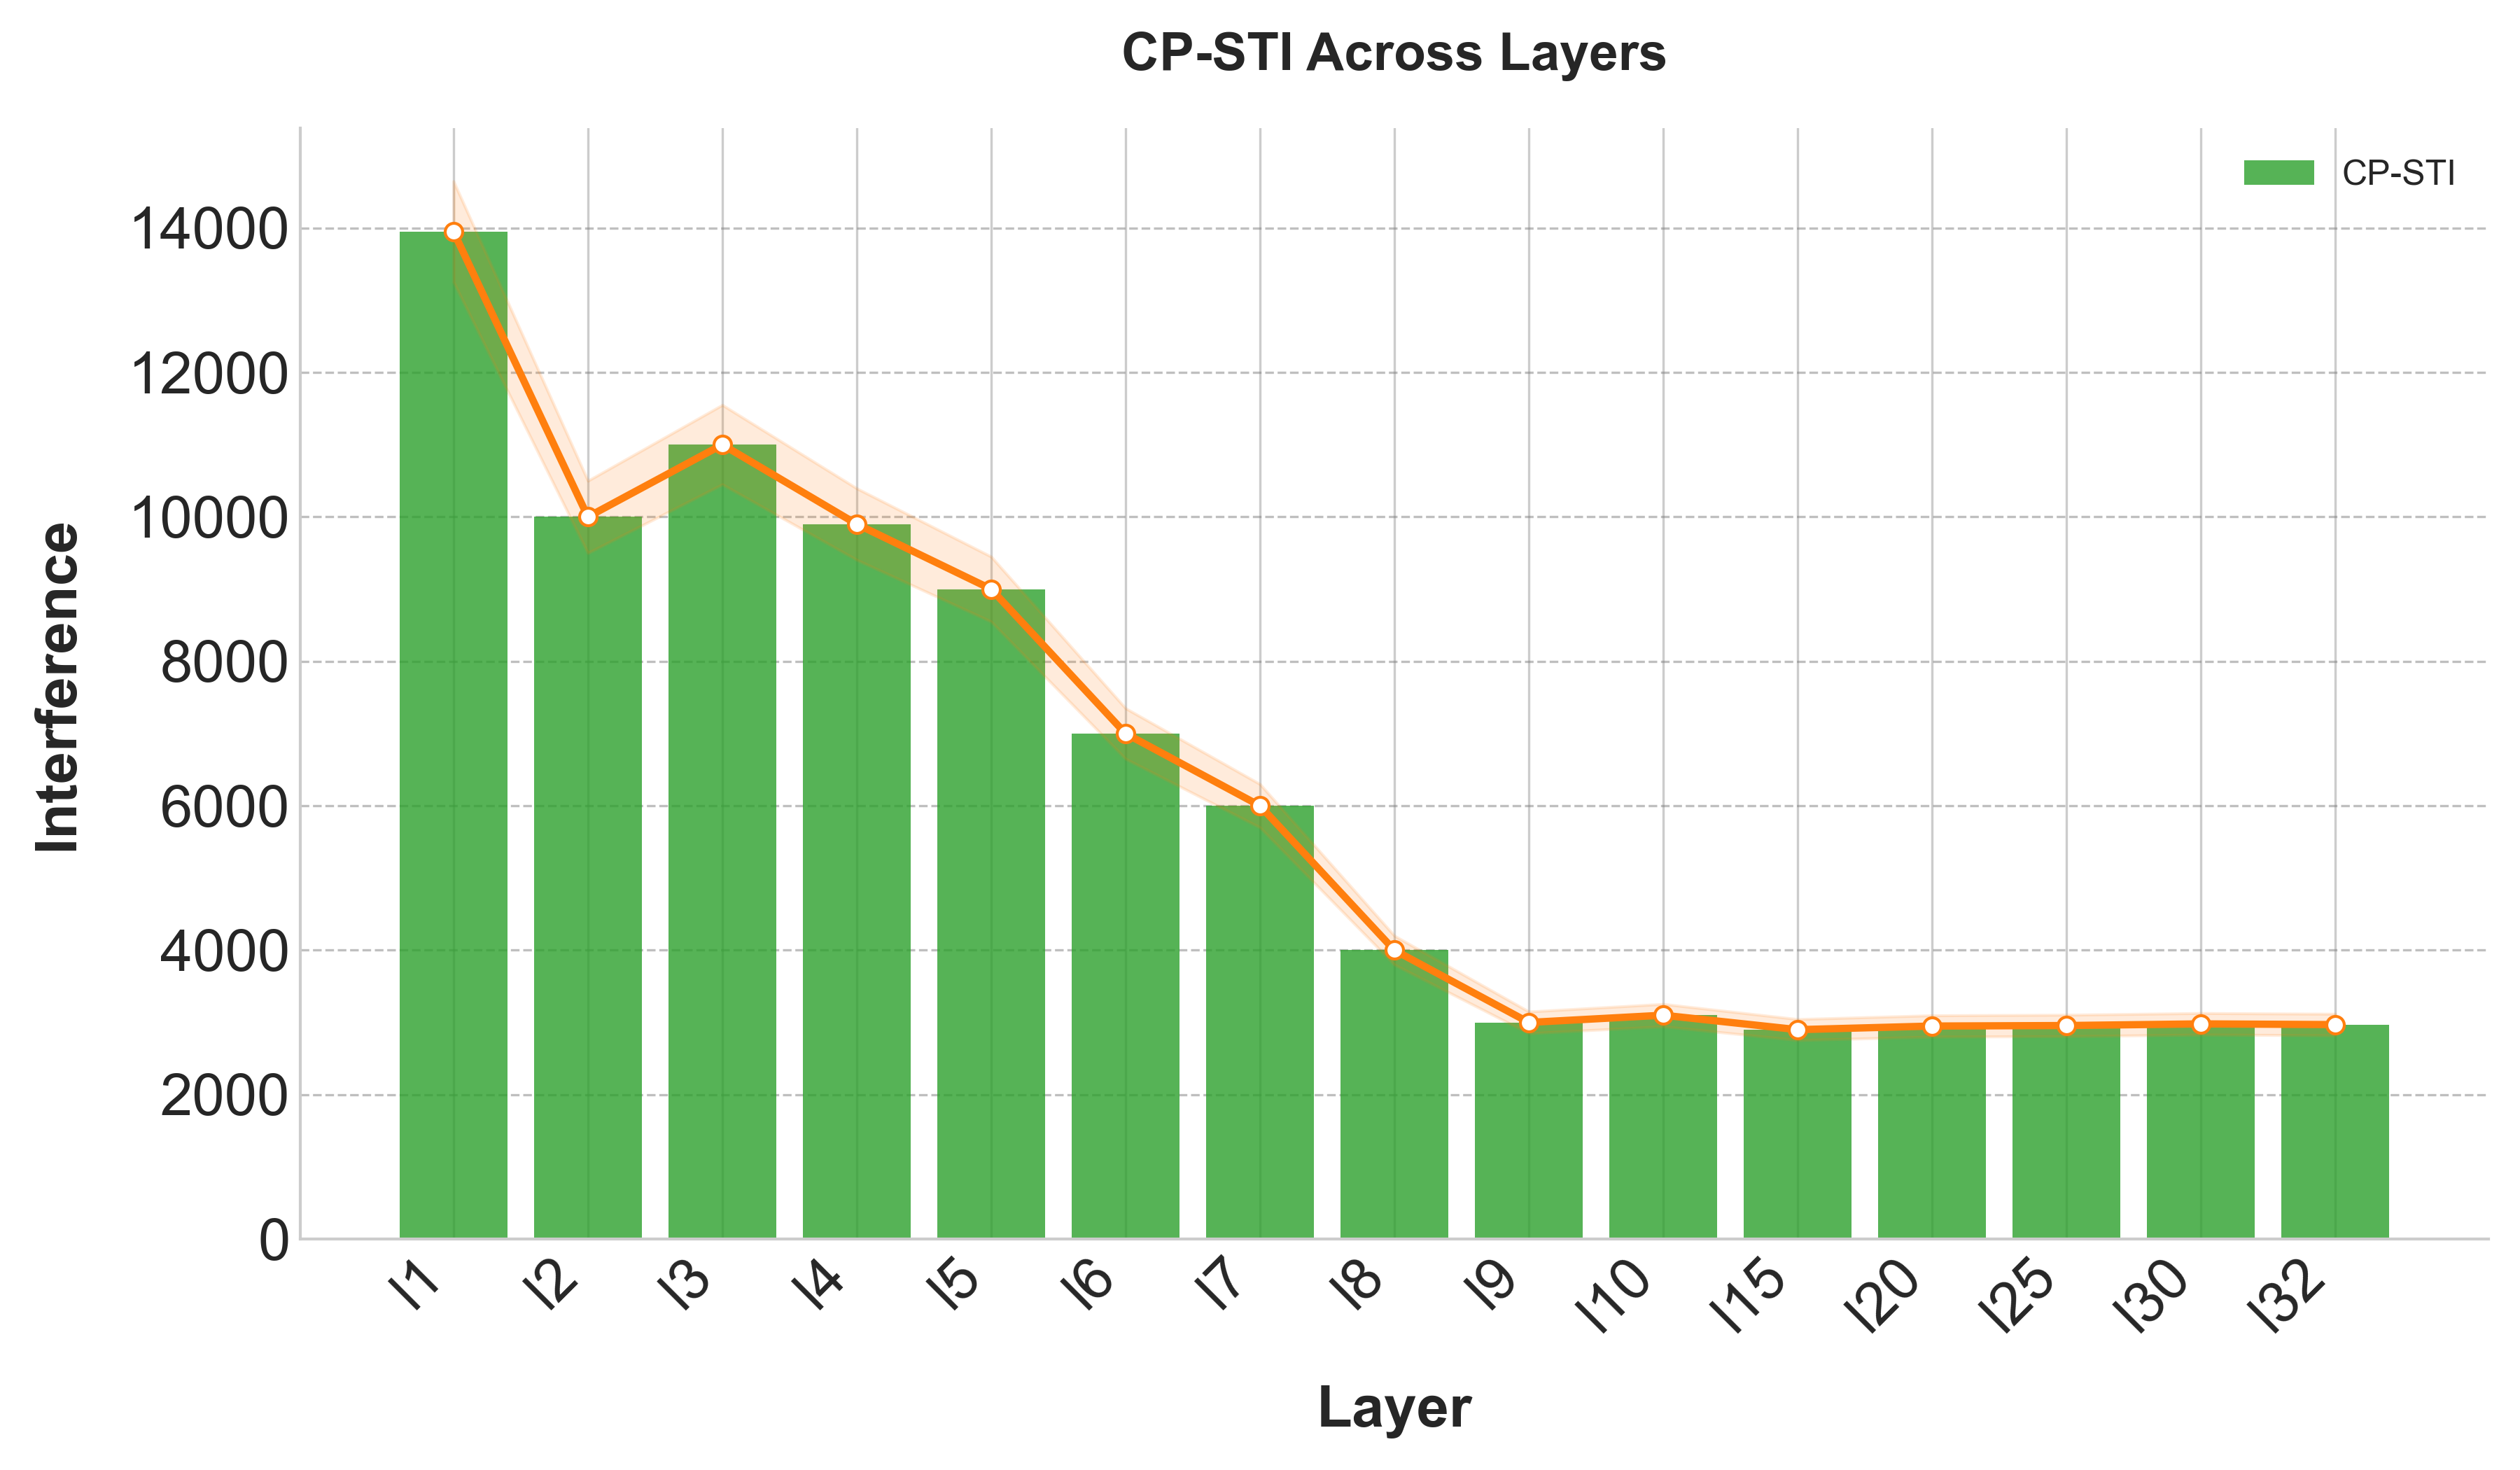
\includegraphics[width=\textwidth]{fig/cp_sti_across_layers.png}
%         \subcaption{CP-STI across 10 layers in the LLama 7B for Math and Code LoRA.}
%         \end{subfigure}
%         \hfill
%         \begin{subfigure}
%             {0.45\textwidth}
%             \centering
%             \includegraphics[width=\textwidth]{
%                 iclr2026/fig/rouge_l_heatmap_with_bolder_lines.png
%             }
%             \subcaption{Best performance for different alpha values. }
%         \end{subfigure}
%         % \caption{The number of clusters and accuracy (ACC) using Phi-3 3B (left)
%         % and Mistral 7B (right).}
%         \label{fig:cluster_performance}
%     \end{figure}





\begin{table}[t]
\centering
\small
\begin{tabular}{llc}
\toprule
Metric & Statistic & Value \\
\midrule
STI & Pearson(layer index, STI) & 0.755 \\
STI & Spearman(layer index, STI) & 0.807 \\
STI & mean(\texttt{qkv\_proj}) / mean(\texttt{o\_proj}) & 1.14 \\
\midrule
CP-STI & Pearson(layer index, log CP-STI) & $-0.006$ \\
CP-STI & Spearman(layer index, log CP-STI) & $-0.063$ \\
CP-STI & mean(\texttt{qkv\_proj}) / mean(\texttt{o\_proj}) & 14.29 \\
CP-STI, column-normalized & Pearson(layer index, CP-STI) & 0.306 \\
CP-STI, column-normalized & Spearman(layer index, CP-STI) & 0.324 \\
CP-STI, off-diagonal & Pearson(layer index, CP-STI) & 0.420 \\
CP-STI, off-diagonal & Spearman(layer index, CP-STI) & 0.533 \\
Diagonal dominance & mean diagonal fraction & 1.000 \\
\bottomrule
\end{tabular}
\caption{Layer-wise interference statistics of STI (TSV merging) and CP-STI (CP merging). For depth correlations, the scores of \texttt{o\_proj} and \texttt{qkv\_proj} are averaged per layer. Raw CP-STI is log10-transformed before computing correlations because its values span several orders of magnitude.}
\label{tab:interference_rebuttal}
\end{table}

Figure~\ref{fig:sti} shows STI across the layers of Phi-3 for five Flan tasks, and Table~\ref{tab:interference_rebuttal} summarizes the layer-wise statistics of STI and CP-STI. Averaged over \texttt{o\_proj} and \texttt{qkv\_proj}, STI increases with depth, both linearly (Pearson correlation with the layer index 0.755) and monotonically (Spearman 0.807), so interference is stronger in deeper layers. This differs from the observation of \citet{gargiulo2025task}, who find interference concentrated in lower layers. STI is also moderately higher on \texttt{qkv\_proj} than on \texttt{o\_proj} (mean ratio 1.14), and the highest values occur on \texttt{qkv\_proj} in layers 17, 19, and 22 to 24.

CP-STI (Appendix~\ref{sec:cp_sti_appendix}, Figure~\ref{fig:cp_sti}) shows a much stronger asymmetry between projections: it is 14.29 times larger on \texttt{qkv\_proj} than on \texttt{o\_proj}, so its magnitude is dominated by the projection type. Its values span several orders of magnitude, and after a log transform the raw score has essentially no depth trend (Pearson $-0.006$, Spearman $-0.063$). Normalizing each column brings CP-STI to a scale comparable with STI and recovers a moderate positive depth trend (Pearson 0.306, Spearman 0.324). The off-diagonal CP-STI, which keeps only interactions between different components, correlates more strongly with depth (Pearson 0.420, Spearman 0.533). The mean diagonal fraction of 1.000 shows that the raw score is almost entirely made up of diagonal terms, which depend on the norms of the factor columns rather than on interactions between components; this is why we also report the column-normalized and off-diagonal variants. Once these scale effects are removed, CP-STI agrees with STI that deeper layers show stronger interference. The same layer-wise pattern holds when CP-STI is computed with the Frobenius instead of the L1 norm (Appendix~\ref{sec:cp_sti_appendix}).





% We study the task interference on each layer according to Eq. (\ref{eq:cp_sti}). As shown in the Fig. \ref{fig:cp_str_interference}, the interference is higher in the lower layer and decreases in the deeper layers. This may indicate that the lower layers capture common features and deeper layers are more specialized for specific tasks. 

\subsection{Rank $R$ of the CP decomposition}
\label{sec:rank_analyse}

        \begin{figure}[t]
        \centering
        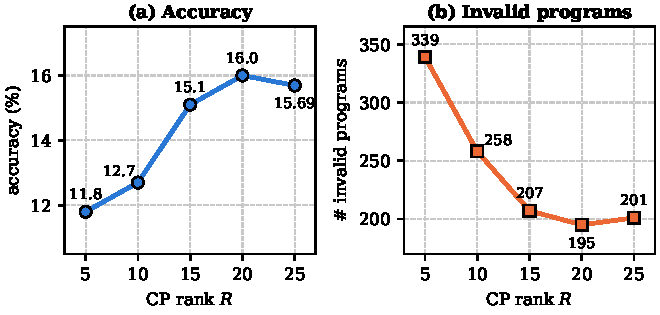
\includegraphics[width=0.62\textwidth]{fig/cp_rank.pdf}
        \caption{Effect of the CP rank $R$ on GSM8K-hard: (a) accuracy and (b) number of invalid programs.}
        \label{fig:CP_rank_performance}
    \end{figure}

    The rank $R$ sets the number of rank-one components in the CP decomposition. \citet{wang2023parameter}
    observed that a larger $R$ can improve performance on cross-modal tasks. Figure~\ref{fig:CP_rank_performance}
    shows the effect of $R$ on GSM8K-hard. Accuracy rises from 11.8\% at rank 5
    to 16.0\% at rank 20 and slightly decreases at rank 25 (15.69\%, the setting
    reported in Table~\ref{tab:math-hard}). The number of invalid programs falls
    from 339 at rank 5 to 195 at rank 20 and changes little at rank 25 (201). A higher rank therefore lets the decomposition
    retain more of each adapter, but the benefit saturates around rank 20.

    % \begin{figure}[h]
    %     \centering
    %     \begin{subfigure}
    %         {0.45\textwidth}
    %         \centering
    %         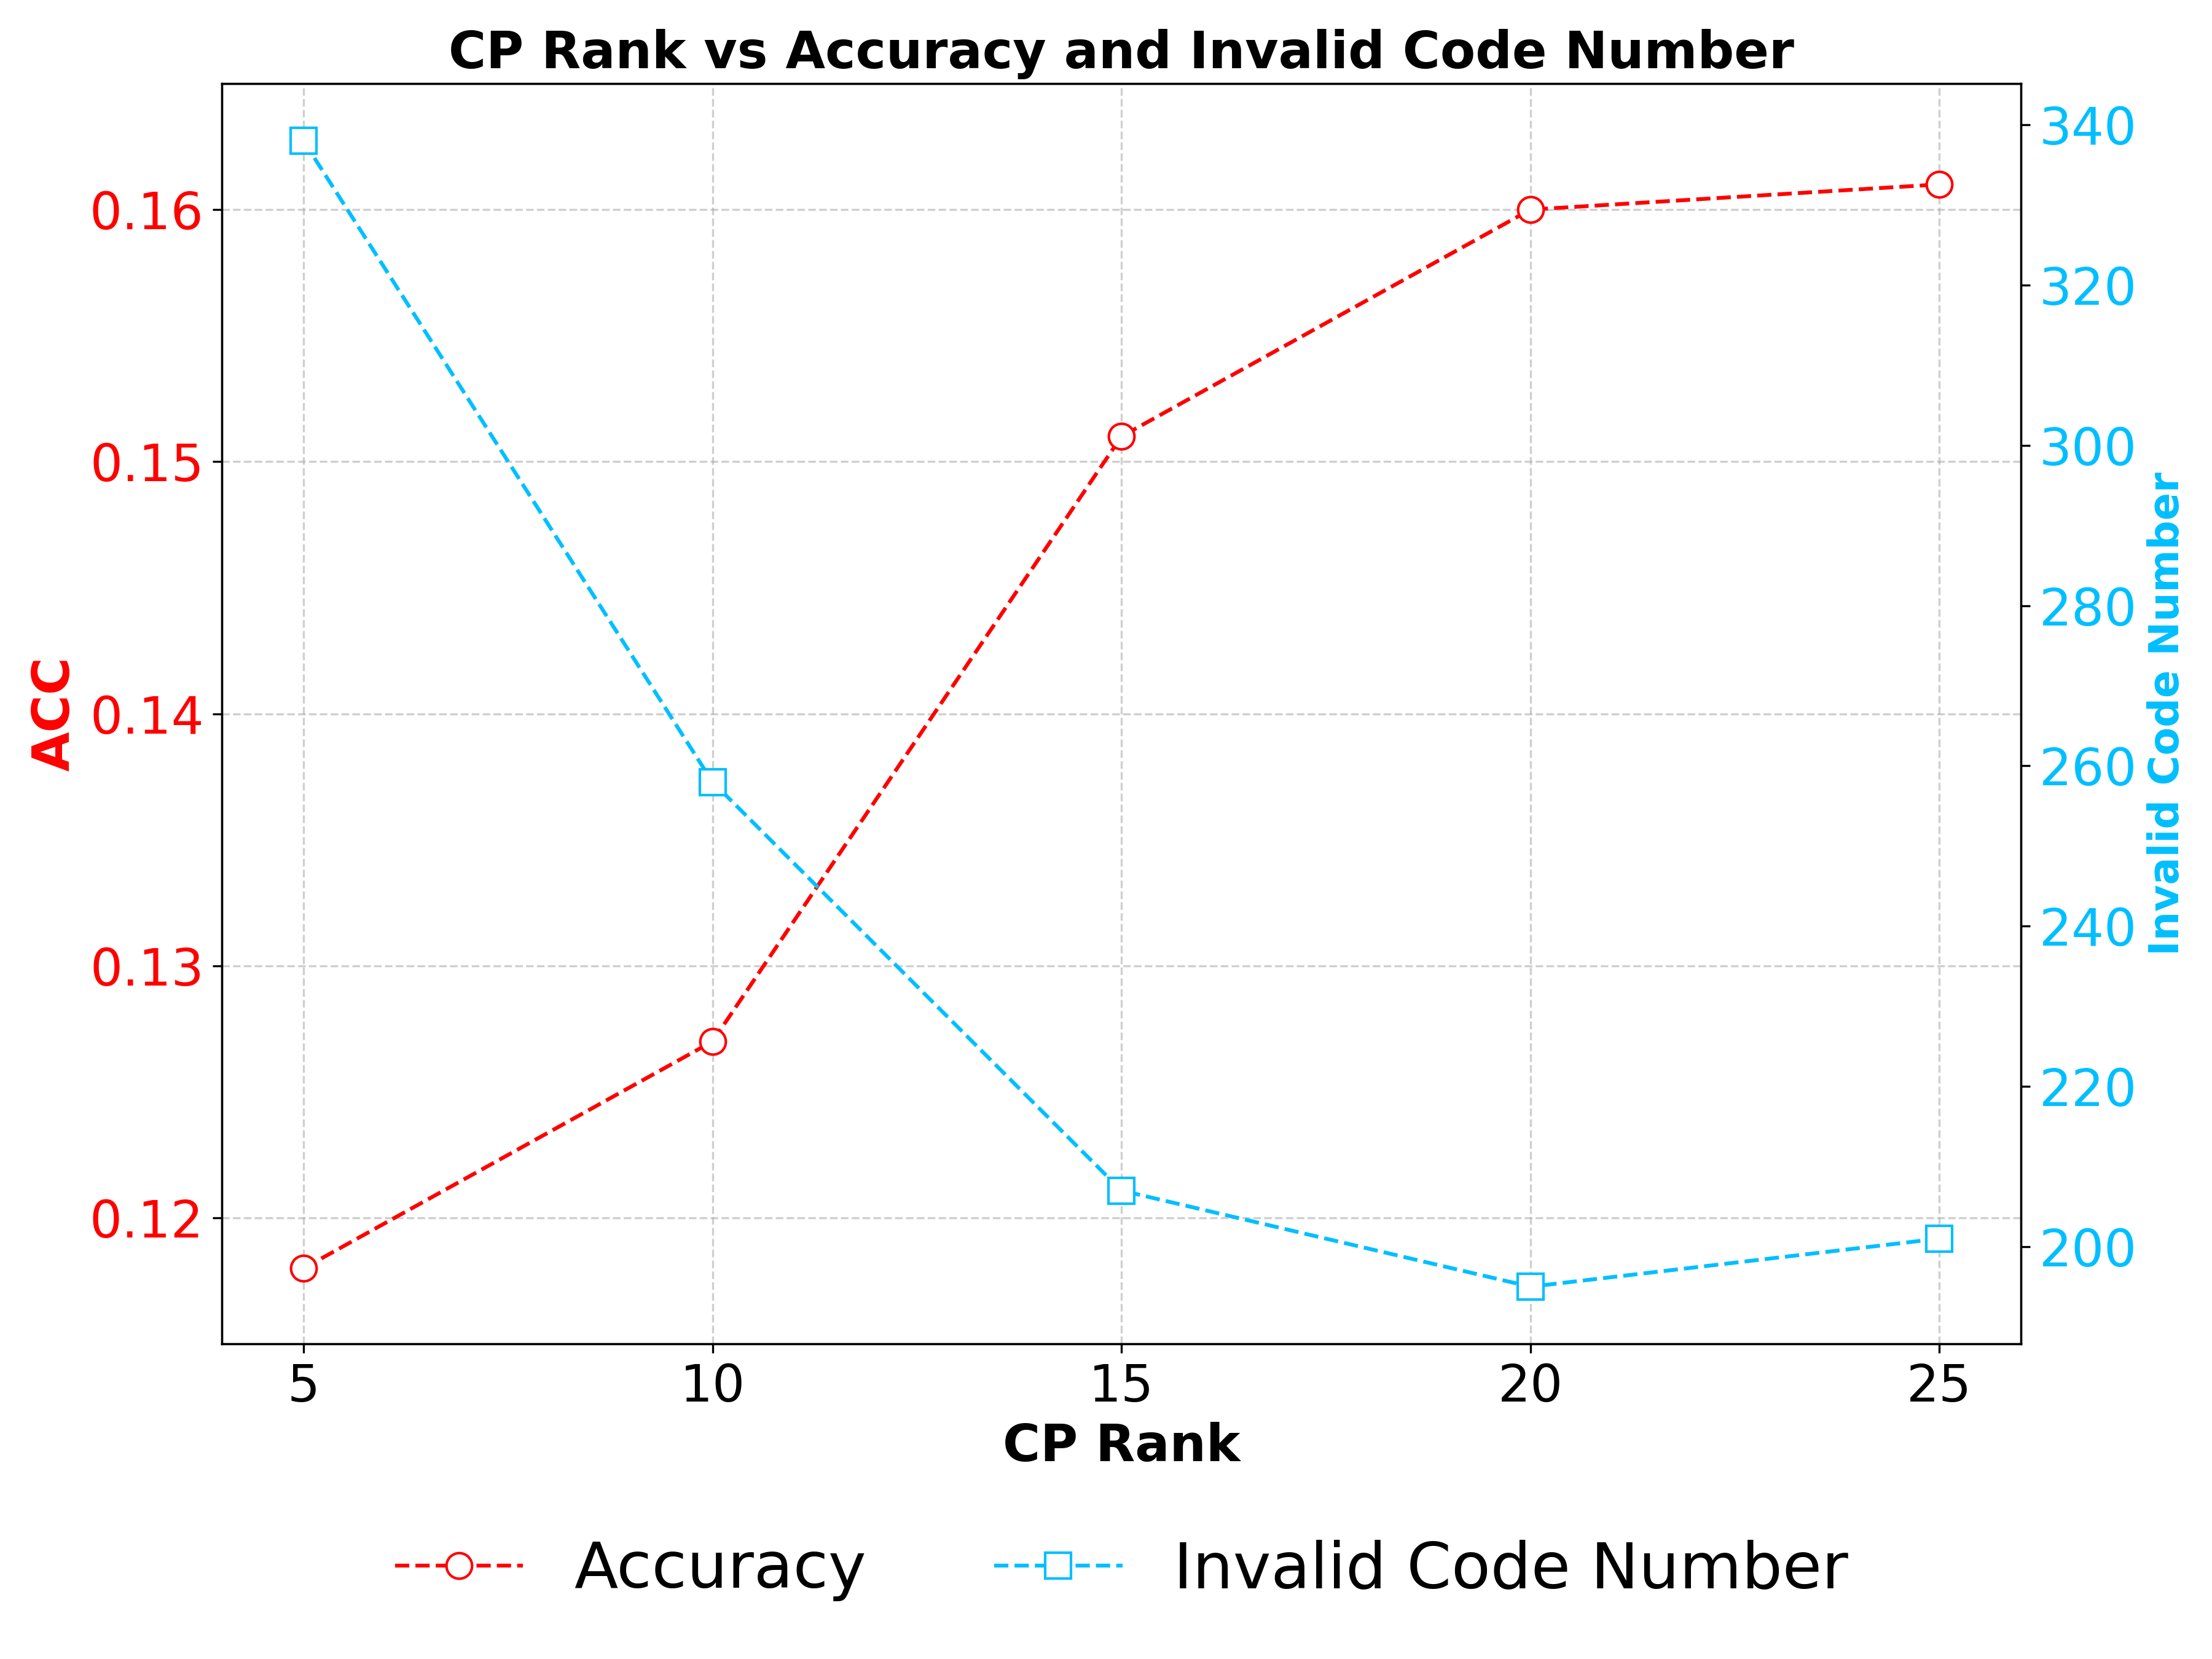
\includegraphics[width=\textwidth]{fig/CP_rank_vs_ACC.png}
    %     \end{subfigure}
    %     \hfill
    %     \begin{subfigure}
    %         {0.45\textwidth}
    %         \centering
    %         \includegraphics[width=\textwidth]{fig/CP_rank_vs_invalid_code.png}
    %     \end{subfigure}
    %     \caption{The impact of CP rank on model performance and generation
    %     quality for the GSM-8K benchmark.}
    %     \label{fig:CP_rank_performance}
    % \end{figure}


\subsection{Scaling factor $\alpha$}

\begin{figure}[t]
\centering
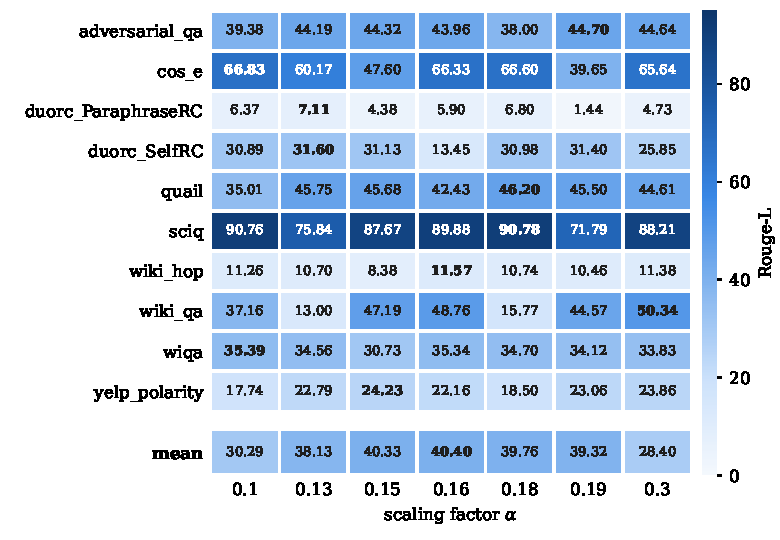
\includegraphics[width=0.6\textwidth]{fig/alpha_heatmap.pdf}
\caption{Rouge-L of CP merging on the 10 held-in Flan tasks for different values of $\alpha$. Bold marks the best value in each row.}
\label{fig:alpha}
\end{figure}

The scaling factor $\alpha$ controls how strongly the merged update is added to the pre-trained weights. Figure~\ref{fig:alpha} reports Rouge-L on the 10 held-in Flan tasks for seven values of $\alpha$ between 0.1 and 0.3. Performance is sensitive to $\alpha$ for all merging methods, including CP merging, Knots, TSV merging, and ISO-C, and the best value differs across tasks. On average, values between 0.15 and 0.18 perform best for CP merging. In all experiments, we select $\alpha$ on a validation set of 1,000 examples, which gives 0.25 for TSV merging and 0.50 for Knots.

\subsection{Computation Cost}



CP merging computes one tensor decomposition per layer, whereas the SVD-based methods compute matrix decompositions. Table~\ref{tab:computation_copmarison} reports the wall-clock time to merge 3, 5, and 10 LoRA adapters of Phi-3 trained on Flan tasks, measured on a single A100 GPU. The cost of TSV merging and Knots grows quickly with the number of adapters and reaches 1320 and 1980 seconds for 10 adapters. CP merging takes between 31 and 58 seconds in all settings, which is more than an order of magnitude faster.
\begin{table}
    \centering
    \begin{tabular}{l|ccc}
    \toprule
      Model  & 3 LoRA & 5 LoRA & 10 LoRA \\
    \midrule
     TSV merging & 350s & 553s & 1320s\\
     Knots & 540s & 780s & 1980s\\
     \midrule
     CP merging & \textbf{31s} & \textbf{38s} & \textbf{58s}\\
     \bottomrule
    \end{tabular}
    \caption{Merging time in seconds for different numbers of LoRA adapters on Phi-3.}
    \label{tab:computation_copmarison}
\end{table}

\section{Discussion}

CP merging as formulated above assumes a fixed set of $N$ adapters stacked into a tensor $\mathcal{T} \in \mathbb{R}^{d_{in} \times d_{out} \times N}$. In practice, new adapters are released after a merged model has been built, and recomputing the full CP decomposition each time becomes costly as $N$ grows.

The decomposition admits a simple incremental update. The input-mode factor $B$ and output-mode factor $C$ describe the subspace shared by the existing adapters, so they can be kept fixed once the initial decomposition is computed. For a new adapter $\Delta_{N+1}$, we then only estimate its task-mode coefficients $\mathbf{a}_{N+1}$ by minimizing the reconstruction error

\begin{equation}
    \min_{\mathbf{a}_{N+1}} \|\Delta_{N+1} - \sum_{r=1}^{R} a_{N+1,r}\, \mathbf{b}_r \otimes \mathbf{c}_r\|_F
\end{equation}

The coefficients $\mathbf{a}_{N+1}$ embed the new task in the existing shared basis without changing the factors of the previous adapters. This replaces a full tensor factorization with a linear least-squares problem. How well a fixed basis represents adapters from very different tasks remains to be evaluated.


\section{Conclusion}
We presented CP merging, a LoRA merging method that stacks the adapters of each layer into a third-order tensor and factorizes them jointly with Canonical Polyadic decomposition. SVD-based methods decompose task matrices one at a time or after concatenation; CP merging instead shares input-mode and output-mode factors across tasks and records task contributions in a separate task mode, which separates shared components from task-specific ones. Across held-in and held-out Flan tasks, zero-shot benchmarks, and math-and-code skill composition, CP merging outperforms TSV merging and Knots and is more than an order of magnitude faster to compute. Uniform merging remains competitive on held-out and zero-shot evaluation, so the main benefit of joint factorization lies in preserving task-specific ability while merging many adapters.



\subsubsection*{Acknowledgments}
Use unnumbered third level headings for the acknowledgments. All
acknowledgments, including those to funding agencies, go at the end of the paper.
Only add this information once your submission is accepted and deanonymized. 

\bibliography{tmlr}
\bibliographystyle{tmlr}

\newpage
\appendix
\section{Appendix}

\subsection{Limitations}

We evaluate CP merging on natural language tasks with Phi-3, Mistral-7B, and LLaMA-7B; larger models are not covered. CP merging outperforms SVD-based LoRA merging, but on held-out and zero-shot tasks uniform merging is competitive and in some cases better, so improving the generalization of LoRA merging remains open. Our Flan experiments merge at most 10 adapters, and merging substantially larger sets of adapters is left for future work.

\paragraph{Use of large language models statement}

We used an LLM to polish the writing. All other content, including the experimental results and analyses, was produced by the authors, who verified the text for accuracy before and after any LLM-assisted editing.




\subsection{Skill Composition Tasks}
\label{sec:skill_composition}

\begin{figure}[h]
        \centering
        \begin{prompt}
            [title={GSM8k vs GSM8k-hard}] { \textcolor{blue}{GSM8k}: A robe takes \textcolor{red}{2} bolts of blue fiber and half that much white fiber. How many bolts in total does it take?

            Reference Answer: 18

            \textcolor{blue}{GSM8k-hard}: A robe takes \textcolor{red}{2287720} bolts of blue fiber and half that much white fiber. How many bolts in total does it take?

            Reference Answer: 3,431,580 }
        \end{prompt}
        \caption{An example from GSM8K and its GSM8K-hard counterpart. GSM8K-hard
        replaces the numbers in the original problem with much larger ones.}
        \label{prompt-verifier}
\end{figure}

    \citet{prabhakar2025lora} use LoRA merging for \textit{skill
    composition}, where a skill is a specific capability that a downstream use
    case requires. For example, solving GSM8K \citep{cobbe2021training} requires
    both \textit{commonsense} and \textit{arithmetic} skills.

    We use this setting to test whether reducing task interference helps
    combine skills, using hard math word problems.
    GSM8K-hard \citep{gao2023pal} contains the same types of problems as GSM8K
    \citep{cobbe2021training} but with more complex arithmetic (Fig.~\ref{prompt-verifier}).
    Following the program-aided approach of \citet{gao2023pal}, the LLM first
    writes a program as an intermediate reasoning step and then executes it with
    a Python interpreter to obtain the answer. The task therefore requires
    mathematical reasoning to analyze the problem and coding to turn the
    reasoning into executable code. Following \citet{prabhakar2025lora}, we
    train one LoRA adapter for math and one for code and merge them.

    \subsubsection{GSM8K-hard Results}
    \begin{table}[h]
        \centering
        \begin{tabular}{l|cc}
            \toprule Model               & ACC             & Invalid Code\\
            \midrule \textbf{BASE}       & 0.0430          & 524          \\
            \textbf{LoRA(math)}          & 0.1175          & 562          \\
            \textbf{LoRA(code)}          & 0.0796          & 159          \\
            \textbf{Multi-task}          & 0.1349          & 413          \\
            \textbf{Uniform}             & 0.1296          & 217          \\
            \textbf{Ties-merging}        & 0.1060          & 223          \\
            \textbf{Task Arithmetic}     & 0.1190          & 232          \\
            \textbf{Ties w/DARE}         & 0.1162          & 227          \\
            \textbf{TA w/DARE}           & 0.1200          & 247          \\
            \textbf{ISO Merging} & 0.0840 & 394 \\
            \textbf{TSV Merging}         & 0.1349          & 224          \\
            
            \textbf{Knots} & 0.1344 & 263\\
            \midrule \textbf{CP merging} & \textbf{0.1569} & 201          \\
            \midrule
            \bottomrule
        \end{tabular}
        \caption{Results on GSM8K-hard. ``Invalid Code'' is the number of
        generated programs that cannot be executed by the Python interpreter.}
        \label{tab:math-hard}
    \end{table}
    Table~\ref{tab:math-hard} reports accuracy and the number of invalid
    programs on GSM8K-hard. The base model reaches an accuracy of only 0.043.
    A LoRA adapter trained on MathQA improves accuracy to 0.1175, and an adapter
    trained on Alpaca-code reduces the number of invalid programs from 524 to 159.
    A single adapter trained on both datasets reaches 0.1349, and uniform merging
    of the two skill adapters reaches 0.1296. TSV merging and Knots obtain similar
    accuracy (0.1349 and 0.1344), with fewer invalid programs for TSV merging
    (224 vs.\ 263). CP merging obtains the highest accuracy of all methods (0.1569),
    2.2 points above TSV merging and the multi-task adapter, and produces 201
    invalid programs. This is fewer than every method except the code-only
    adapter (159), which has much lower accuracy (0.0796). CP merging thus combines
    the math and code skills with less loss of either than the other merging
    methods.





\subsection{Additional Interference Analysis}
\label{sec:cp_sti_appendix}

Figure~\ref{fig:cp_sti} shows CP-STI across the layers of Phi-3 for the same five Flan tasks as Figure~\ref{fig:sti}.

\begin{figure}[h]
    \centering
    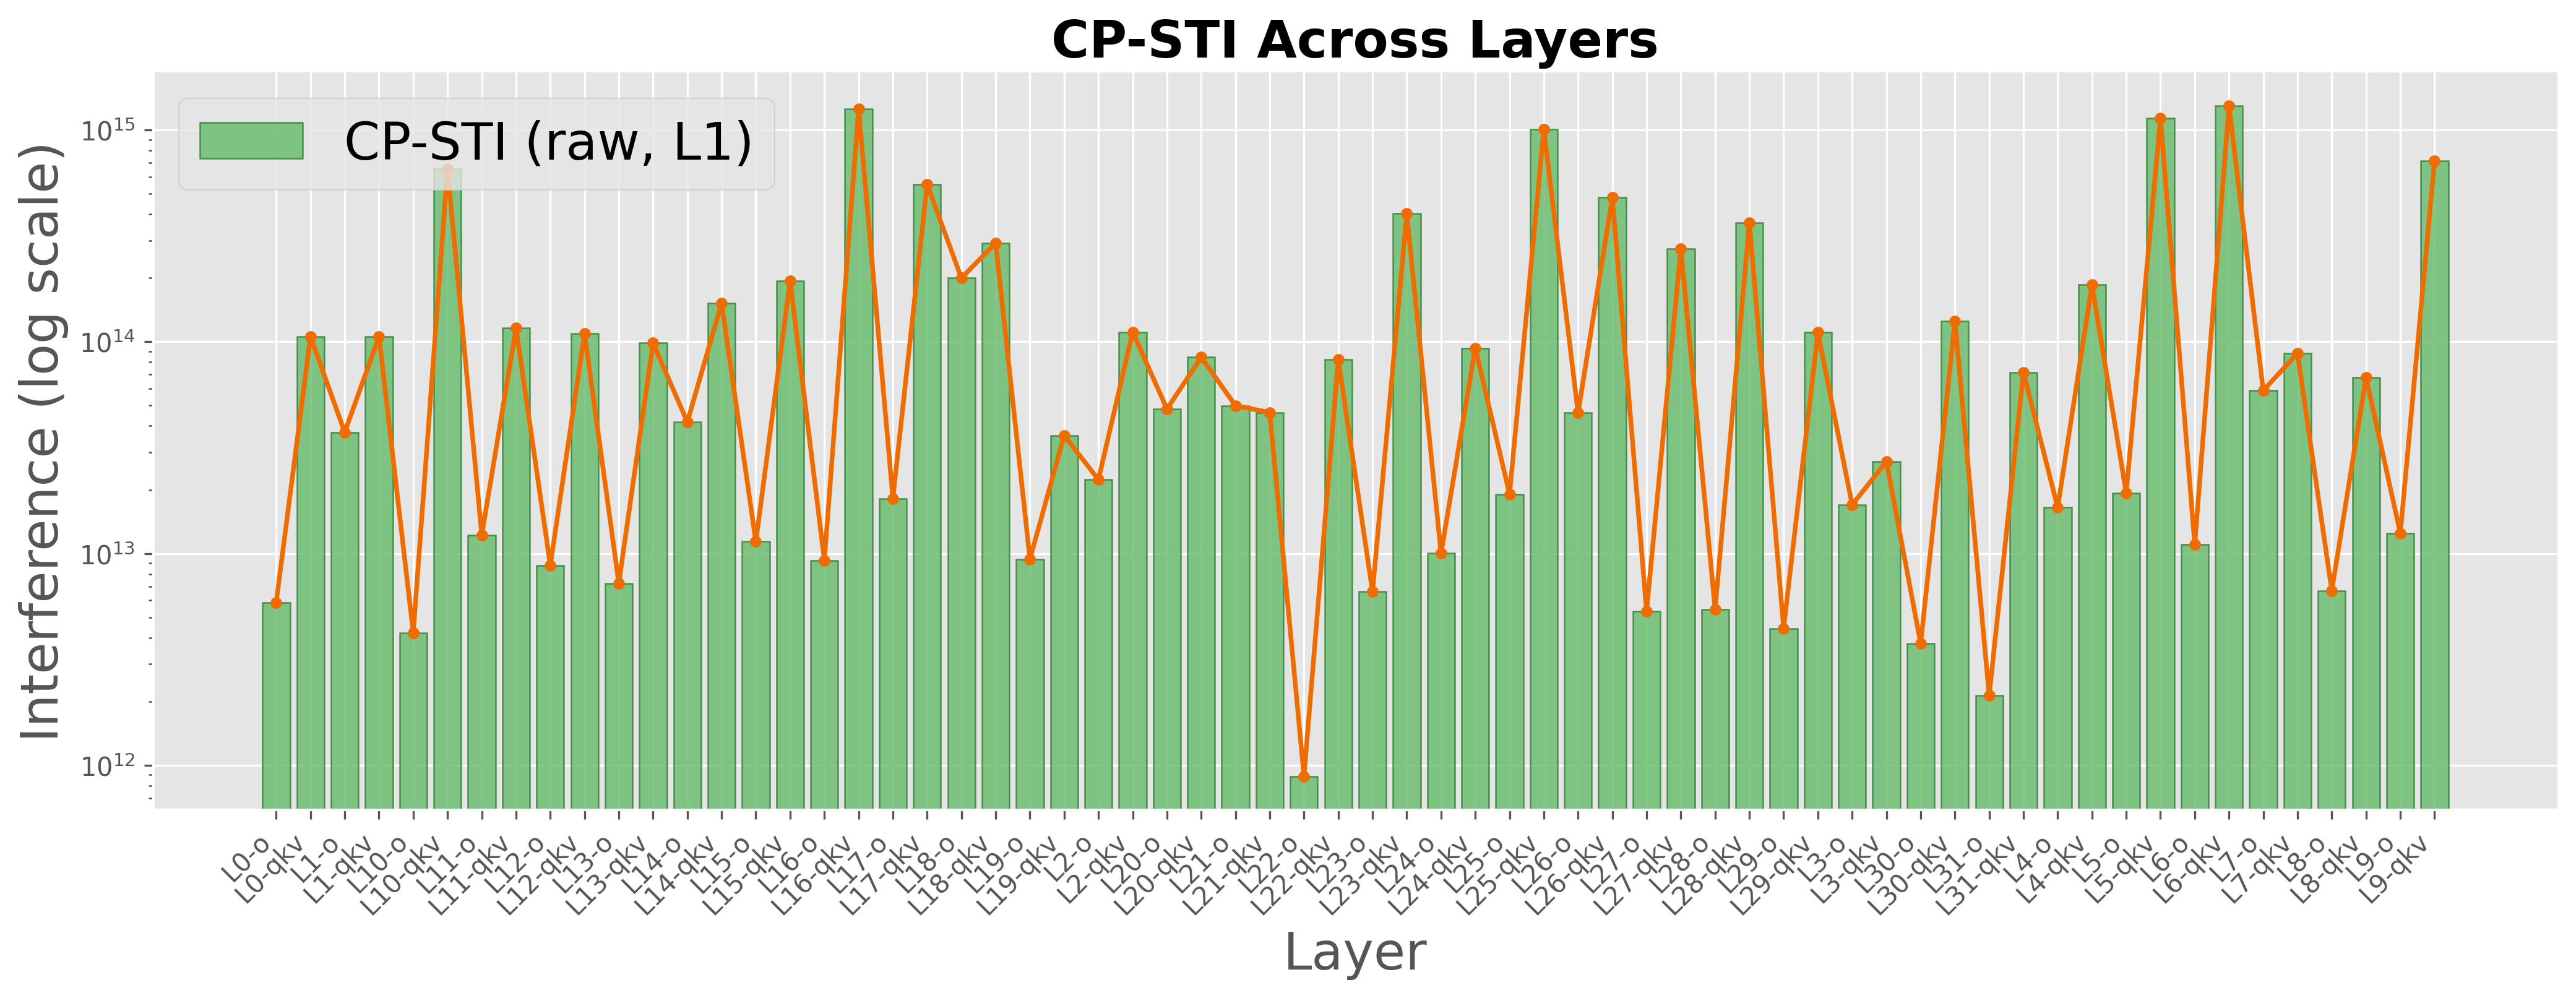
\includegraphics[width=0.7\linewidth]{fig/cpmergeafter_cp_sti_across_layers_beautified.png}
    \caption{CP-STI of CP merging across layers on 5 Flan tasks.}
    \label{fig:cp_sti}
\end{figure}

\begin{figure}
    \centering
    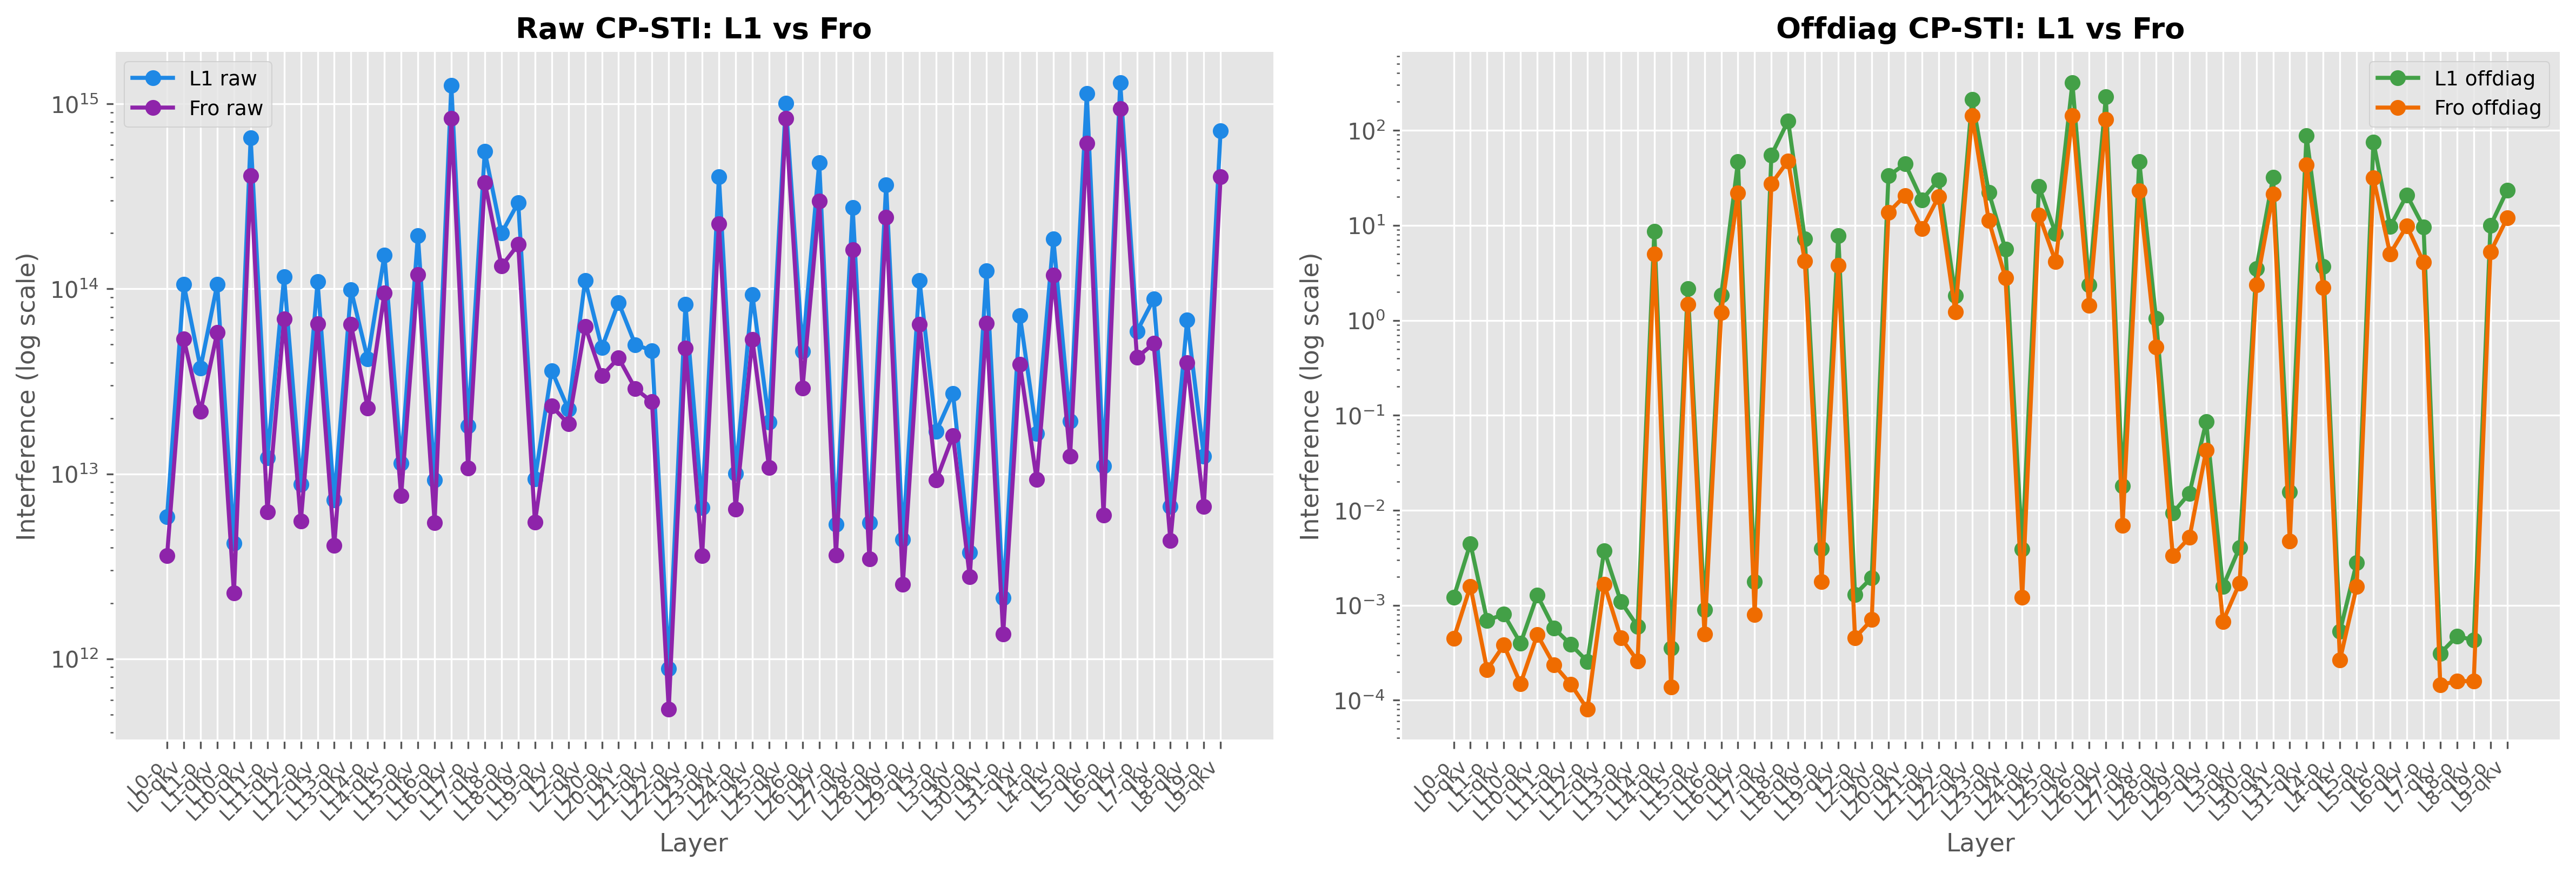
\includegraphics[width=\linewidth]{fig/cpmergeafter_cp_sti_l1_vs_fro_across_layers_beautified.png}
    \caption{CP-STI across layers computed with the L1 and Frobenius norms. Left: raw CP-STI. Right: off-diagonal CP-STI.}
    \label{fig:cp-sti-l1-f}
\end{figure}

Figure~\ref{fig:cp-sti-l1-f} compares CP-STI computed with the L1 and Frobenius norms. Both norms produce the same layer-wise pattern, with peaks and valleys at the same layers. Frobenius values are smaller, but the ranking of layers is preserved, and the off-diagonal variants of the two norms also track each other closely. The layer-wise conclusions above therefore do not depend on the choice of norm.

\subsection{Cross-task similarity of SVD and CP factors}

Similarity between the $U$ and $V$ matrices of different experts reflects how much the experts share. To examine how SVD represents cross-task relations, we compute the pairwise cosine similarity of the $U$ and $V$ matrices of five task experts (Figure~\ref{fig:SVD_visualization}). The off-diagonal similarities are low, so the SVD factors of different tasks share little common orientation. The $V$ similarities (right) in particular show that the input-side directions of different tasks are nearly orthogonal. Merging such adapters directly projects different tasks onto misaligned subspaces, which is consistent with the information conflict that SVD-based merging must resolve.

% This observation provides the primary motivation for our CP-based approach, which overcomes this 'basis-mismatch' by factorizing all tasks simultaneously within a higher-order tensor framework, thereby ensuring a consistent and aligned parameter space.



\begin{figure}[h]
        \centering
        \begin{subfigure}
            \centering
            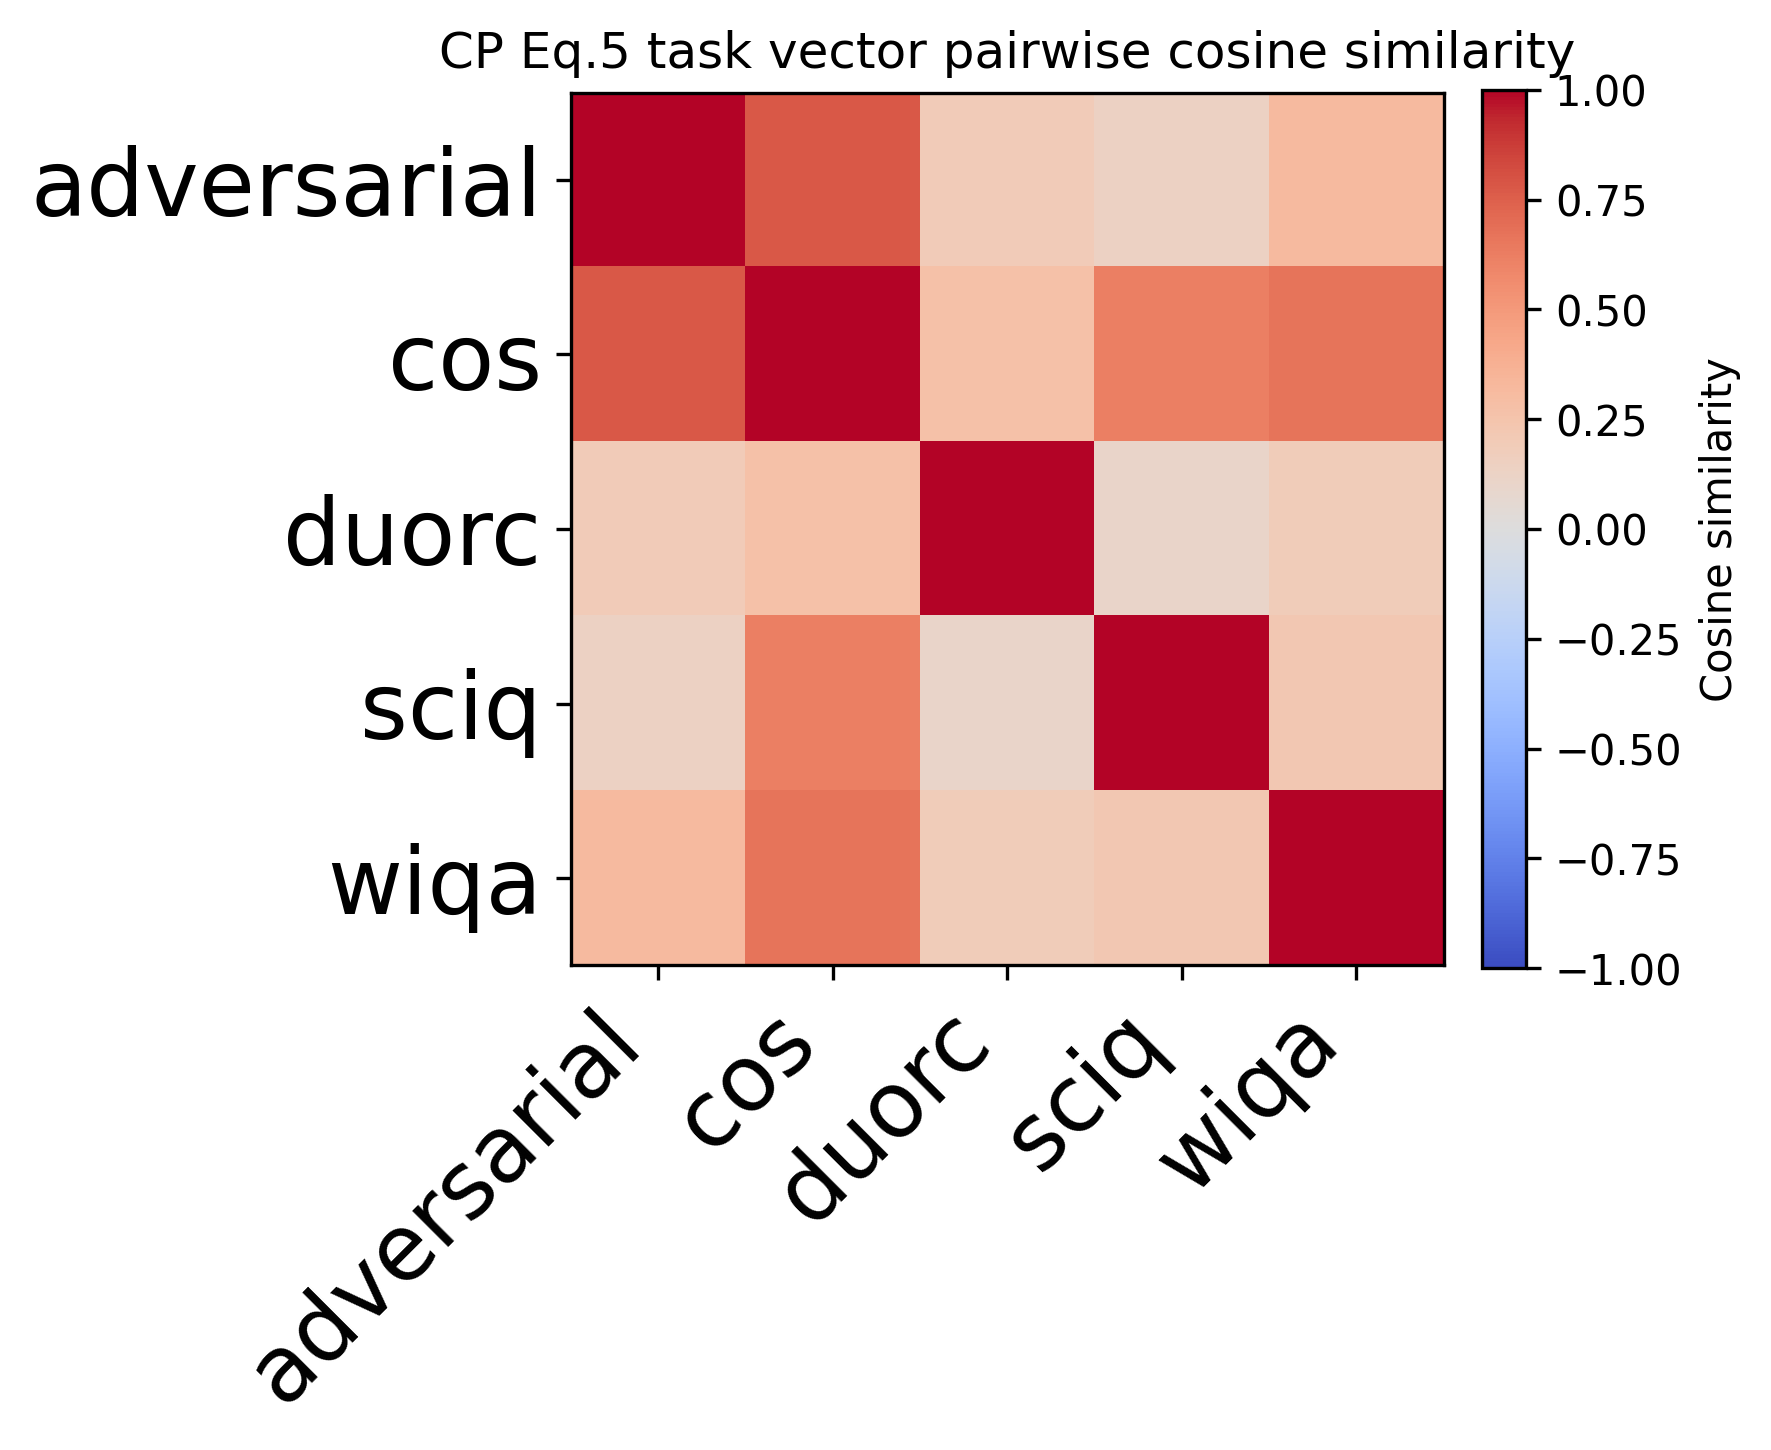
\includegraphics[width=0.28\textwidth]{fig/cpmergeafter_cp_eq5_task_matrix_cosine_similarity_model.layers.0.self_attn.o_proj.png}
        \end{subfigure}
        \hfill
        \begin{subfigure}
            \centering
            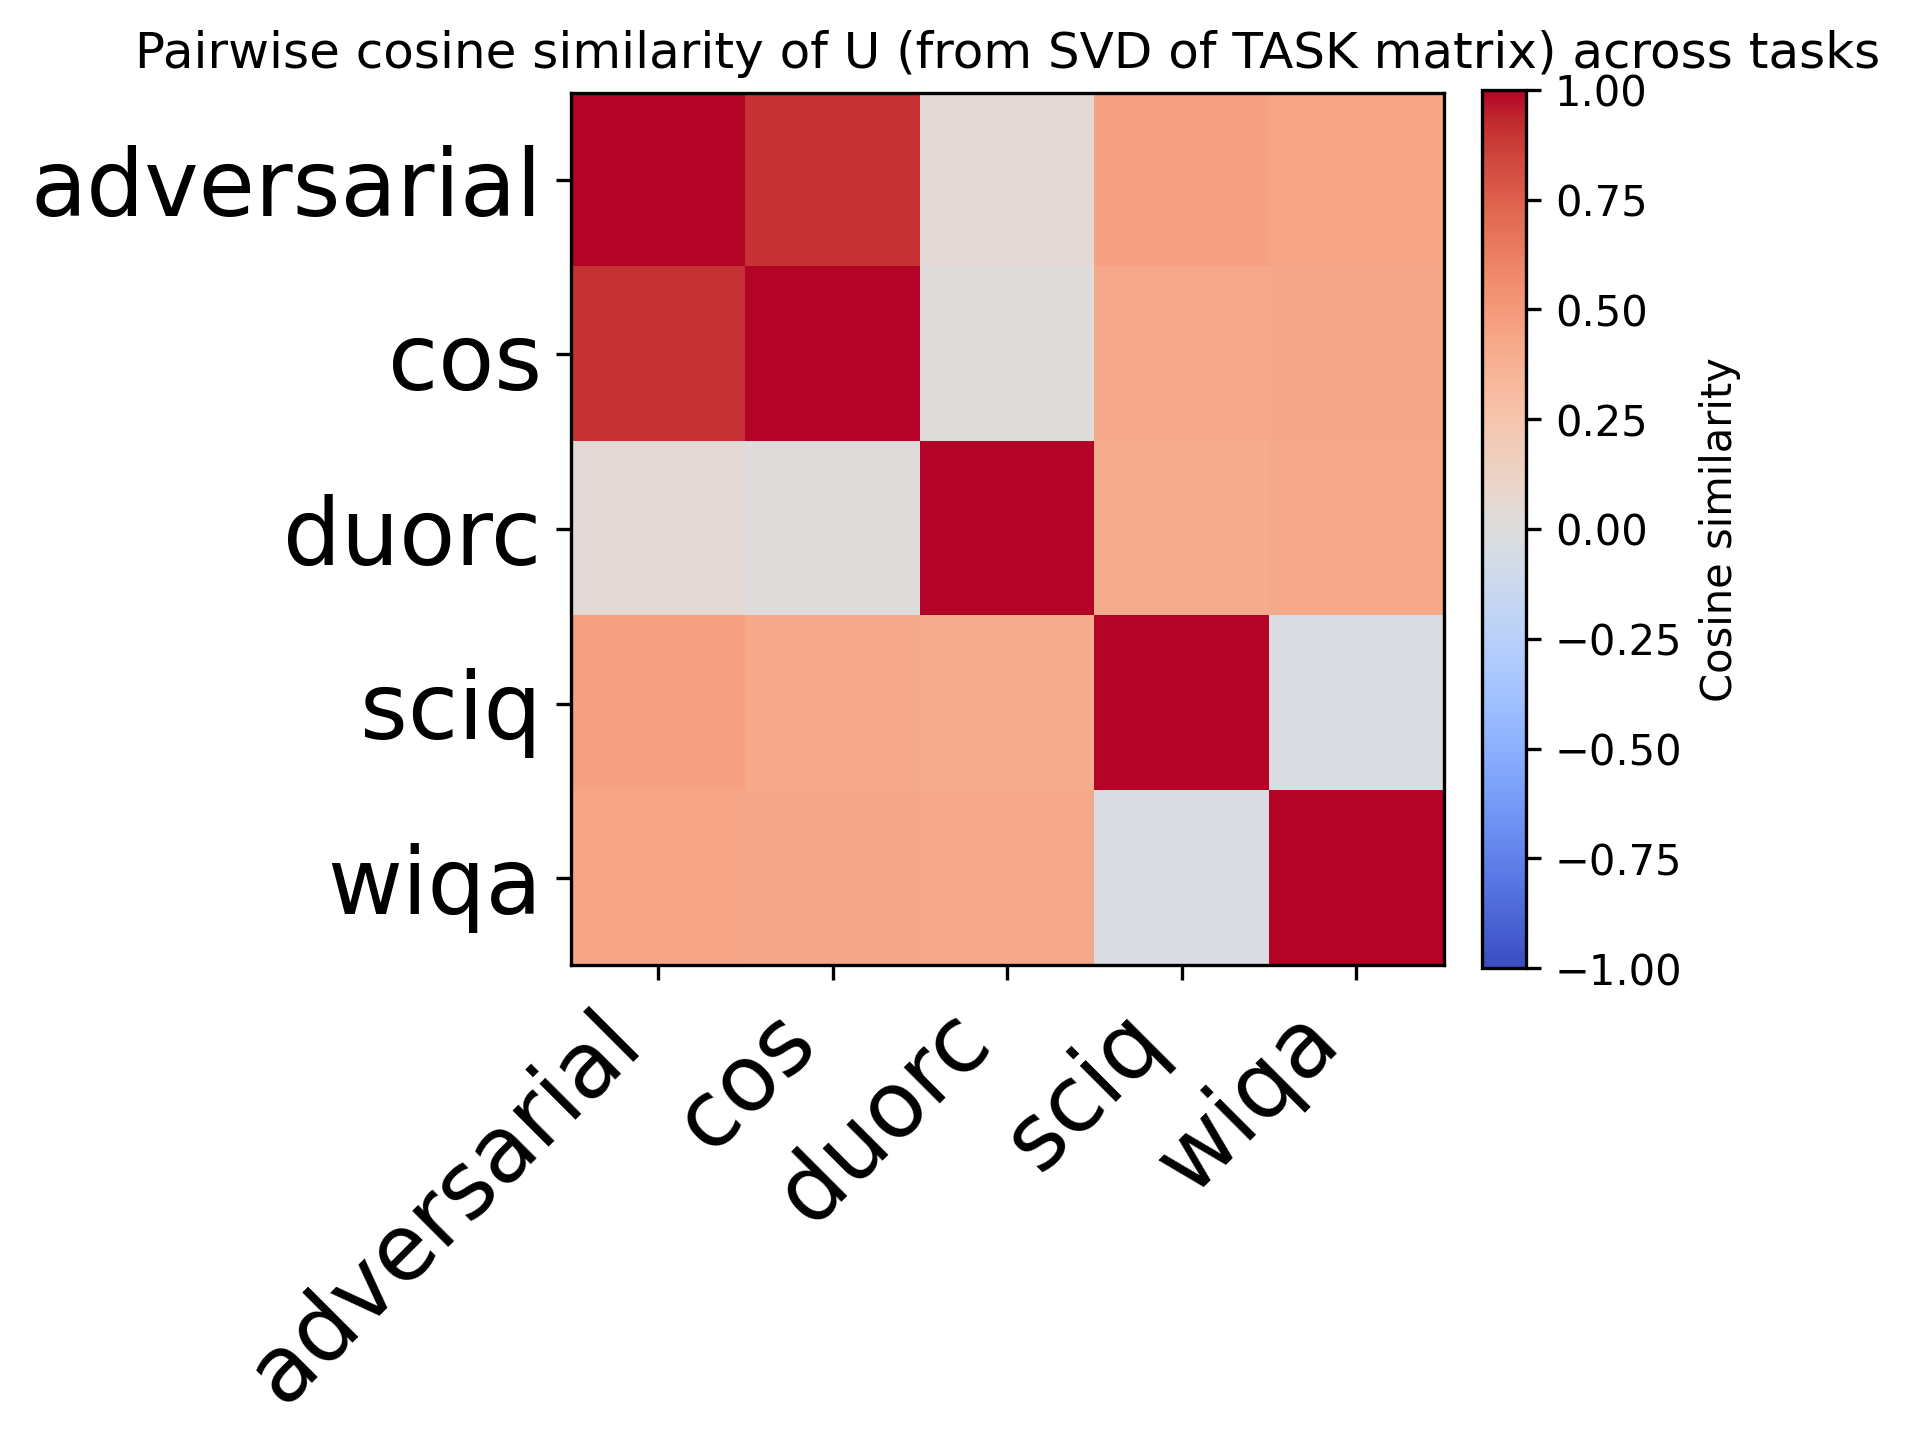
\includegraphics[width=0.30\textwidth]{fig/cpmergeafter_svd_u_cosine_similarity.png}
            % \subcaption{The number of clusters and accuracy (ACC) using Phi-3 3B}
        \end{subfigure}
        \hfill
        \begin{subfigure}
            \centering
            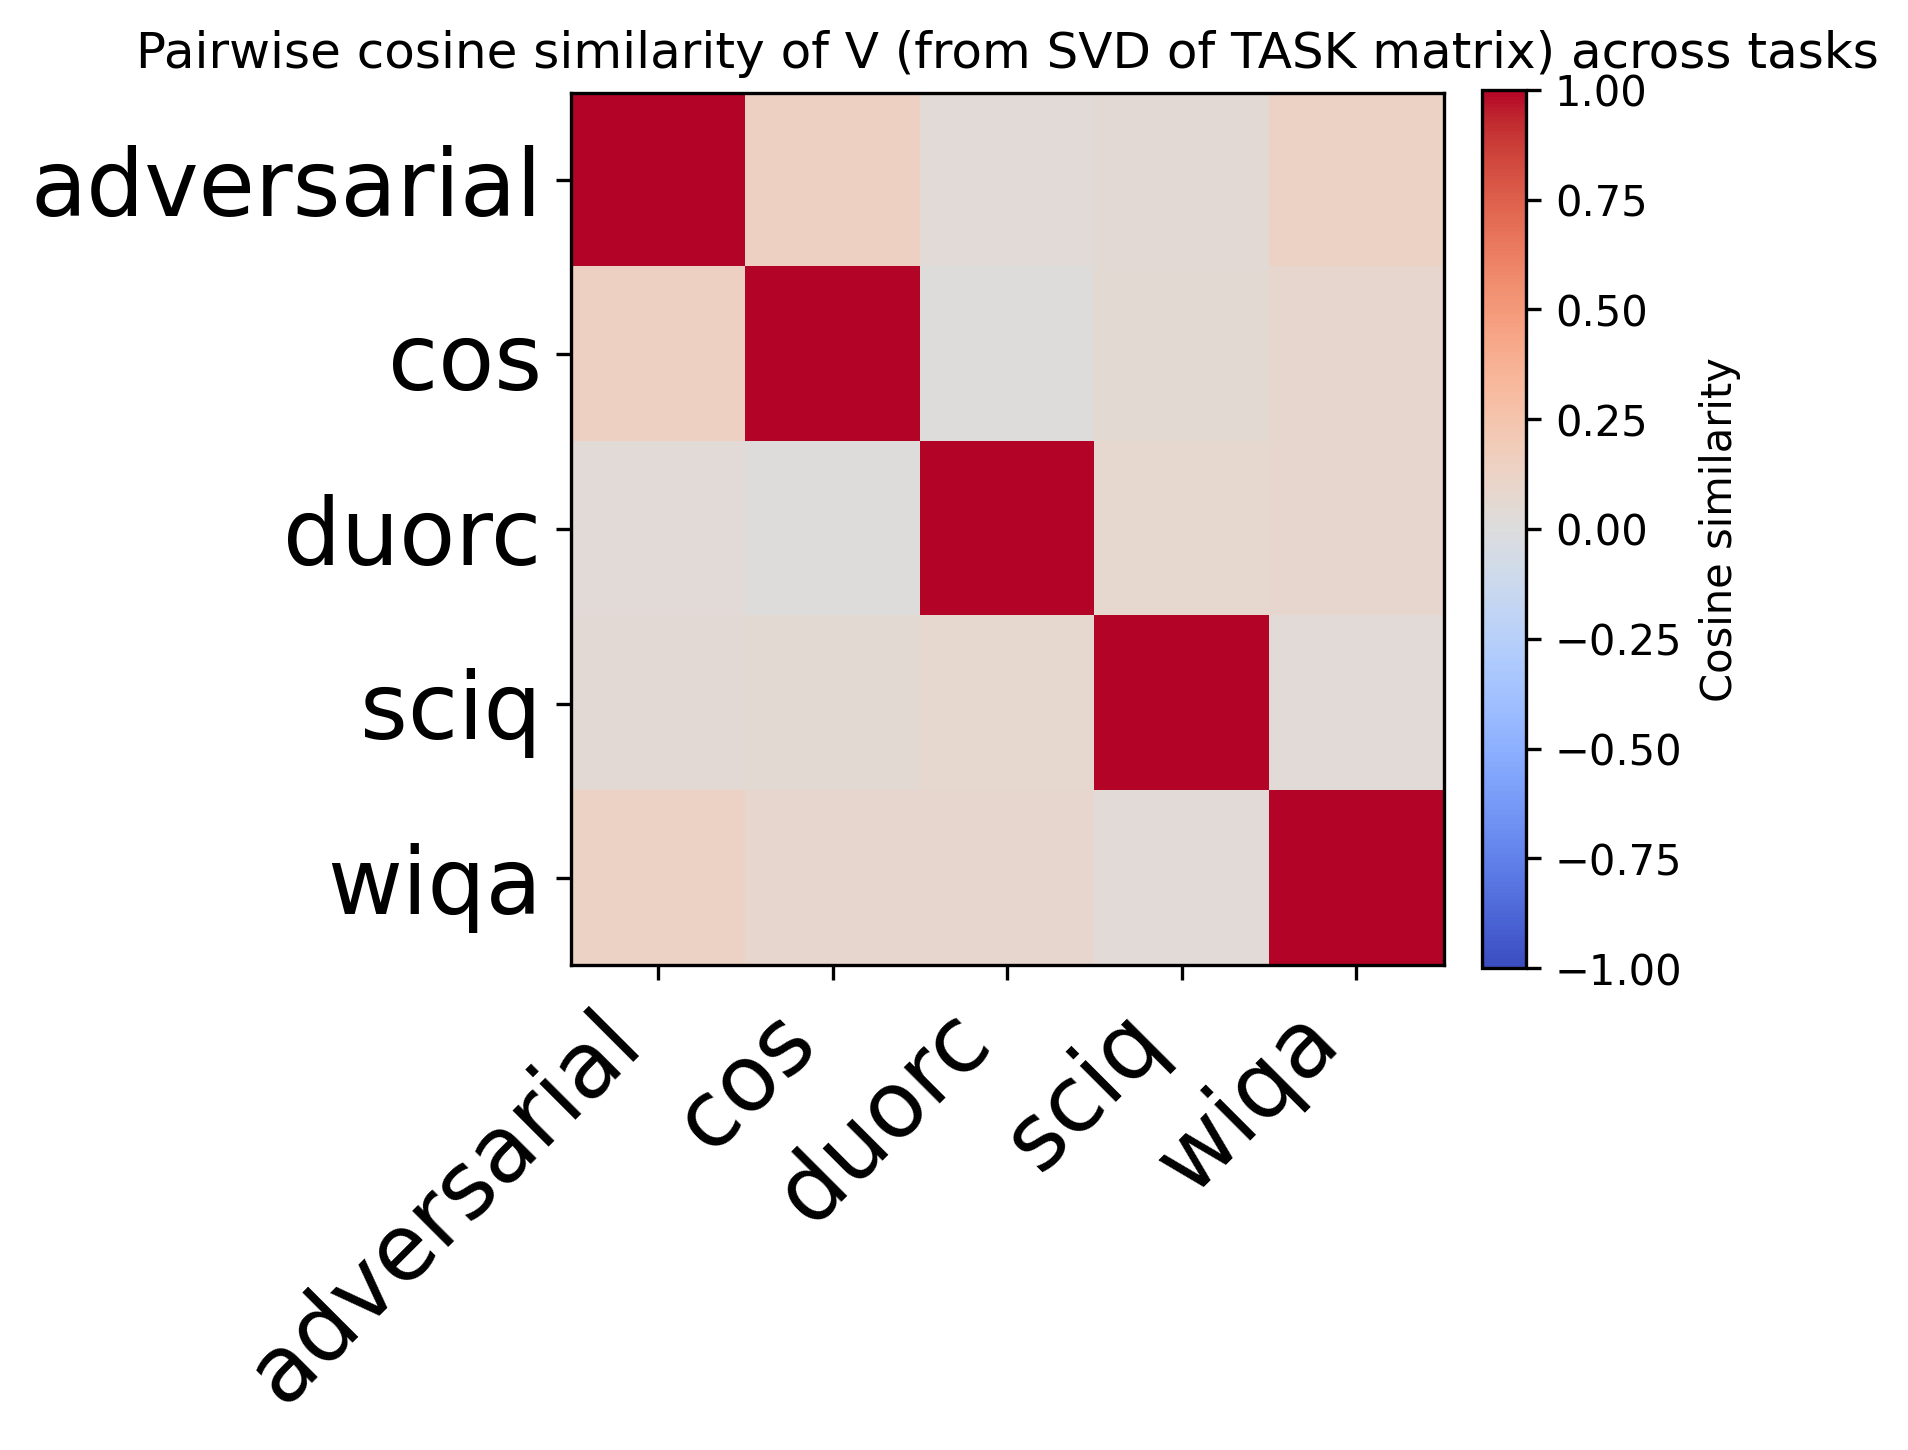
\includegraphics[width=0.30\textwidth]{fig/cpmergeafter_svd_v_cosine_similarity.png}
            % \subcaption{The number of clusters and accuracy (ACC) using Mistral 7B}
        \end{subfigure}
        \caption{Pairwise cosine similarity between five task experts in layer 0 of Phi-3. Left: similarity between the task matrices $\Delta_i$ and $\Delta_j$ reconstructed from CP factors (Eq.~\ref{eq:cp_form}). Middle: similarity between the SVD $U$ matrices. Right: similarity between the SVD $V$ matrices.}
        \label{fig:SVD_visualization}
    \end{figure}

We quantify this comparison with the off-diagonal entries of the pairwise expert-similarity matrices (Figure~\ref{fig:cp_svd_offdiag}). We compare the task matrices reconstructed from CP factors (Eq.~\ref{eq:cp_form}) with the SVD representations $U$, $V$, and their mean. On the tested layer, the CP and SVD similarities are only moderately correlated (Pearson 0.578 with $U$, 0.486 with $V$, and 0.576 with $(U+V)/2$; Spearman 0.305, 0.353, and 0.377), and their mean absolute difference is 0.204. CP and SVD therefore induce different cross-task dependence structures. The SVD dependence is also unbalanced across factors (mean off-diagonal similarity 0.348 for $U$ and 0.068 for $V$), whereas the CP reconstruction yields a single dependence pattern at the level of the full task matrix (0.349). CP decomposition thus models cross-task interaction through factors shared by all tasks and retains dependence information that the separate SVD bases do not.

\begin{figure}[h]
    \centering
    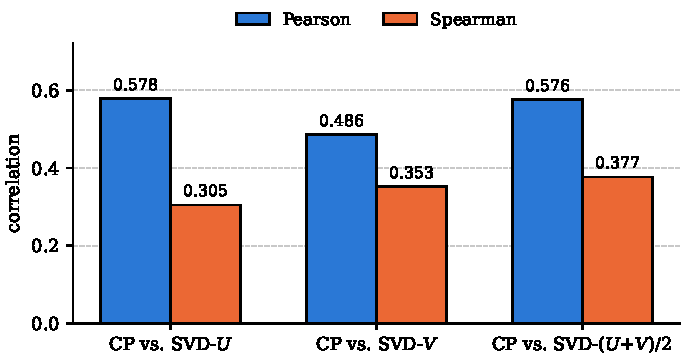
\includegraphics[width=0.65\linewidth]{fig/cp_svd_offdiag.pdf}
    \caption{Correlation between the off-diagonal entries of the CP-based and SVD-based expert-similarity matrices, pooled over all layers.}
    \label{fig:cp_svd_offdiag}
\end{figure}


\subsection{Experimental Setting for Flan and Zero-shot Tasks}
\label{sec:exp_setting}

\subsubsection{Implementation Details}

We compute the CP decomposition with the \texttt{parafac} solver of the open-source library TensorLy\footnote{\url{https://tensorly.org/dev/modules/generated/tensorly.decomposition.parafac.html}}, which uses alternating least squares (ALS) with random initialization and a fixed rank $R$, and stops when the change in error falls below a tolerance \texttt{tol} or after \texttt{n\_iter\_max} iterations.


\begin{figure}[h]
    \centering
    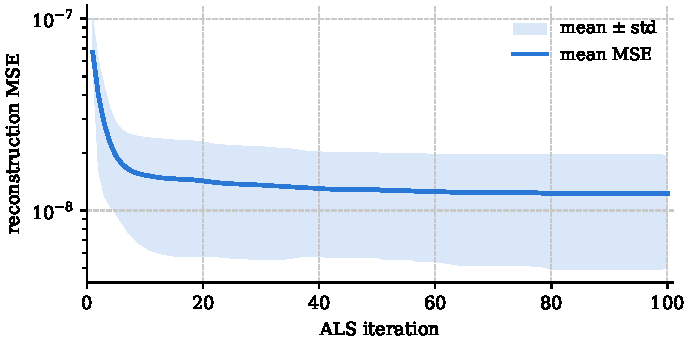
\includegraphics[width=0.65\linewidth]{fig/cpd_convergence.pdf}
    \caption{Convergence of the CP decomposition for a library of 5 LoRA experts on Phi-3: reconstruction error per ALS iteration, averaged over layers (mean $\pm$ std).}
    \label{fig:cpd_convergence}
\end{figure}

To monitor convergence, we record the reconstruction error after each ALS iteration $t$ as the mean squared error $\text{MSE}_t = \|\mathcal{T} - \hat{\mathcal{T}}_t\|_F^2 / |\mathcal{T}|$, where $\hat{\mathcal{T}}_t$ is the reconstruction and $|\mathcal{T}|$ the number of entries; it is computed from the relative reconstruction error reported by TensorLy. Figure~\ref{fig:cpd_convergence} shows the error averaged over layers. The error decreases monotonically and saturates after a moderate number of iterations, so the ALS optimization in Algorithm~\ref{al:factorizing} converges stably in our setting.

% \begin{figure}[h]
%         \centering
%         \begin{subfigure}
%             \centering
%             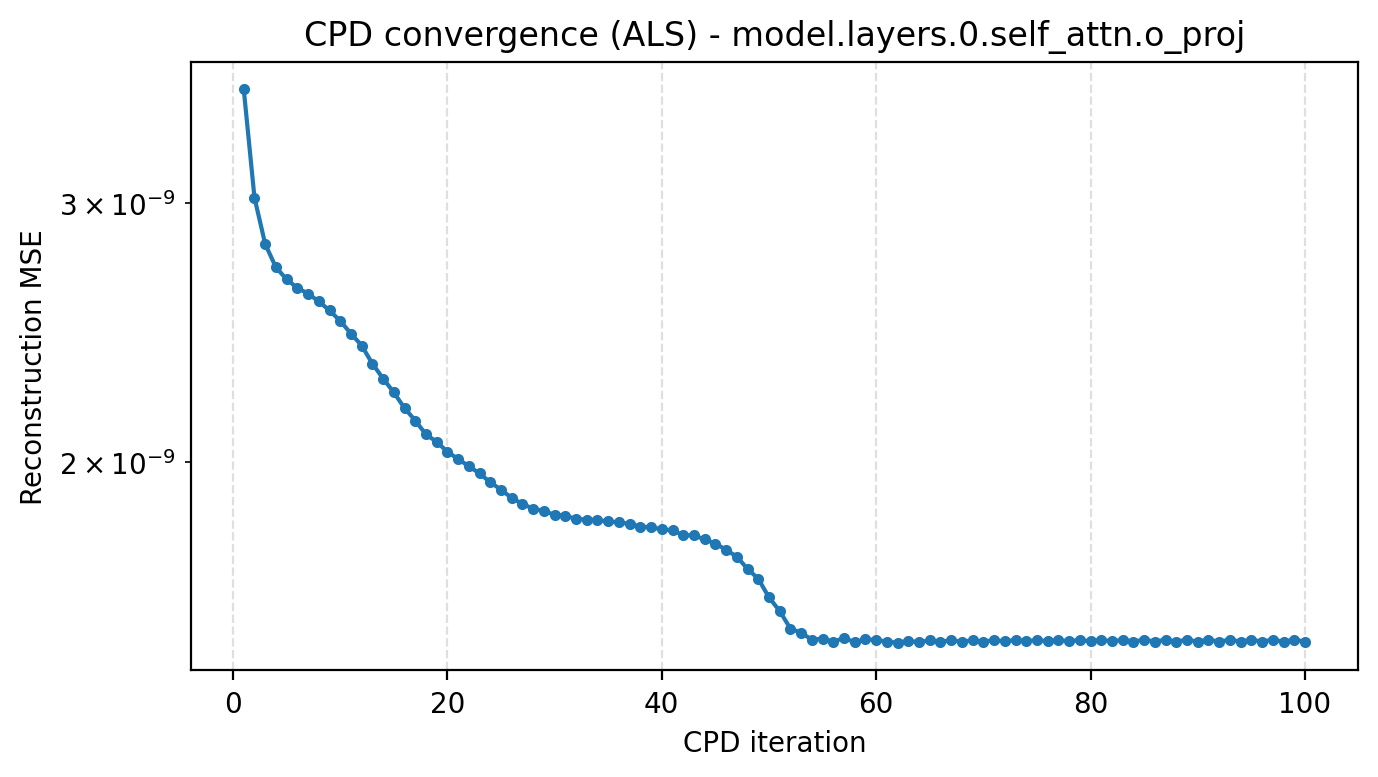
\includegraphics[width=0.3\textwidth]{fig/cpmergeafter_cpd_convergence_model.layers.0.self_attn.o_proj.png}
%             % \subcaption{The number of clusters and accuracy (ACC) using Phi-3 3B}
%         \end{subfigure}
%         \hfill
%         \begin{subfigure}
%             \centering
%             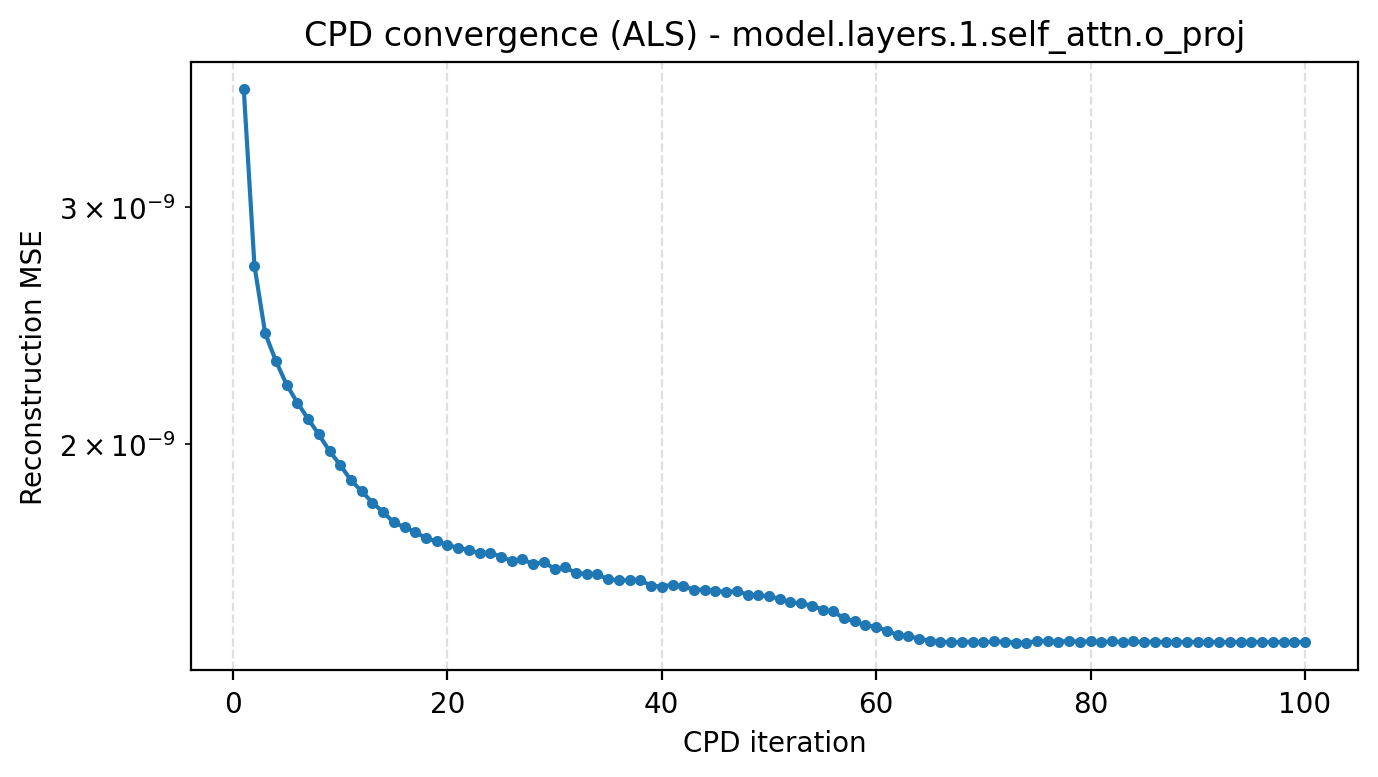
\includegraphics[width=0.3\textwidth]{fig/cpmergeafter_cpd_convergence_model.layers.1.self_attn.o_proj.png}
%             % \subcaption{The number of clusters and accuracy (ACC) using Mistral 7B}
%         \end{subfigure}
%         \hfill
%         \begin{subfigure}
%             \centering
%             \includegraphics[width=0.3\textwidth]{
%                 fig/cpmergeafter_cpd_convergence_model.layers.1.self_attn.o_proj.png}
%             % \subcaption{Clustering based on the sentence embedding. We visualize  100 samples in each cluster.} 
%         \end{subfigure}
%         \caption{Left: accuracy versus number of clusters with Phi-3. Middle: accuracy versus number of clusters with Mistral-7B. Right: sentence embeddings of 100 samples per cluster.}
%         \label{fig:cluster_performance}
%     \end{figure}


\subsubsection{Datasets and Running Environment Setting}

We build the LoRA library from FlanV2, an instruction-tuning collection designed to scale task diversity and model size \citep{chung2024scaling}. We select 256 tasks \citep{longpre2023flan}, most of them from P3 \citep{bach2022promptsource} and Flan2021 \citep{wei2021finetuned}, and train one LoRA adapter independently on each task.

We use Phi-3 \citep{abdin2024phi} and Mistral-7B (\texttt{mistralai/Mistral-7B-v0.1}) \citep{jiang2023mistral} as backbones and apply LoRA only to the attention layers. Unless stated otherwise, multi-task and single-task adapters use LoRA rank 4, dropout 0.05, and learning rate $10^{-4}$, and each adapter is trained for 5 epochs on an H100 or A100 GPU. For the C-LoRA library (Appendix~\ref{sec:clora}), we encode instructions with \texttt{sentence-transformers/sentence-t5-xxl}, fit k-means on a random 20\% of the data, and assign every sample to its nearest cluster.

\subsubsection{Held-in and Held-out Tasks}
\label{sec:10_held_in}

From the 256 tasks of \citet{ostapenko2024towards}, we randomly select 10 held-in tasks and 3 held-out tasks, following \citet{arnobexploring}.

\paragraph{Held-in tasks}

\begin{itemize}
    \item wiqa\_what\_is\_the\_final\_step\_of\_the\_following\_process
    \item sciq\_Multiple\_Choice
    \item adversarial\_qa\_droberta\_answer\_the\_following\_q
    \item duorc\_SelfRC\_question\_answering
    \item cos\_e\_v1\_11\_description\_question\_option\_id
    \item wiki\_qa\_Is\_This\_True\_
    \item quail\_description\_context\_question\_text
    \item wiki\_hop\_original\_explain\_relation
    \item duorc\_ParaphraseRC\_build\_story\_around\_qa
    \item yelp\_polarity\_reviews\_0\_2\_0
\end{itemize}

\paragraph{Held-out tasks}
\begin{itemize}
    \item glue\_sst2\_2\_0\_0
    \item dream\_read\_the\_following\_conversation\_and\_answer\_the\_question
    \item race\_middle\_Read\_the\_article\_and\_answer\_the\_question\_no\_option\_
\end{itemize}

\subsection{Cross-layer analysis}



\begin{figure}[h]
    \centering
    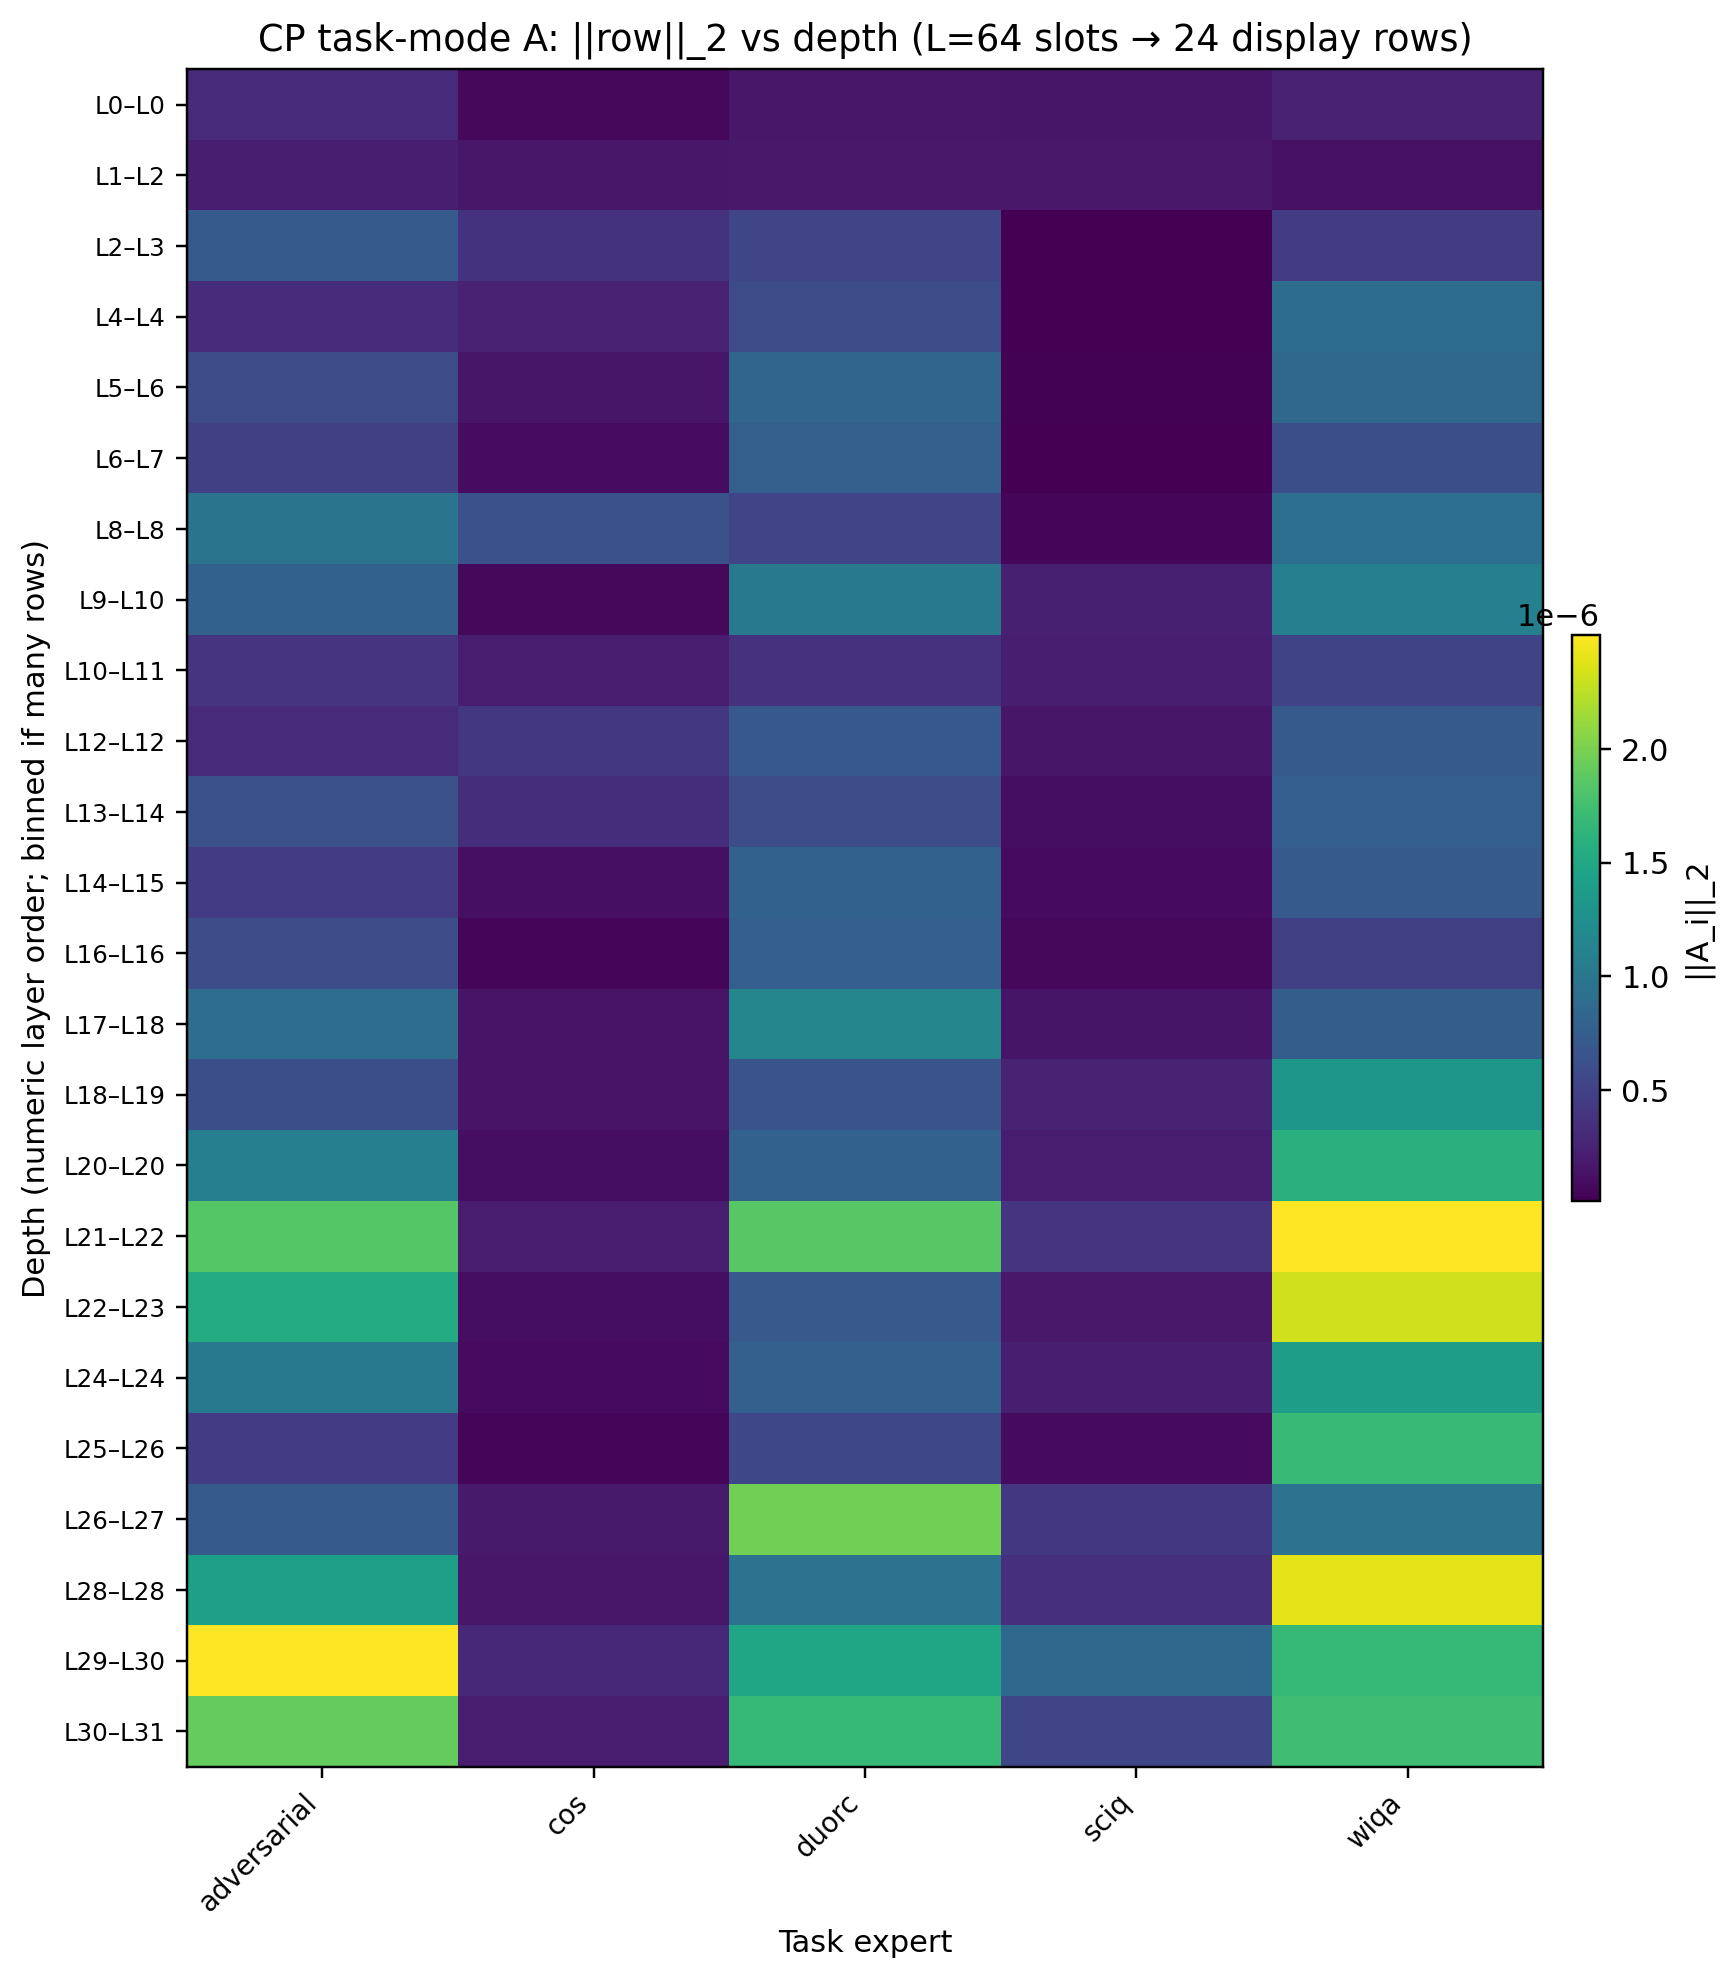
\includegraphics[width=0.5\linewidth]{fig/cpmergeafter_cross_layer_task_A_l2_heatmap.png}
    \caption{L2 norm of each task's row of the task-mode factor $A$ across layers and projections.}
    \label{fig:l2_norm_cross_layer}
\end{figure}

We summarize how a task uses the CP components of a layer by the L2 norm of its row in $A$ and by the entropy of the magnitude-normalized row, which measures whether the task relies on a few components or spreads over many. Figure~\ref{fig:l2_norm_cross_layer} shows that task influence varies with depth. Some tasks have small norms in most layer and projection slots, while others concentrate in later blocks, especially in the deeper \texttt{o\_proj} and \texttt{qkv\_proj} slots. The decomposition therefore reflects a structured dependence on depth rather than independent noise per layer, and the importance of a task depends on the layer and projection, forming visible bands rather than flat profiles.


\begin{figure}[h]
    \centering
    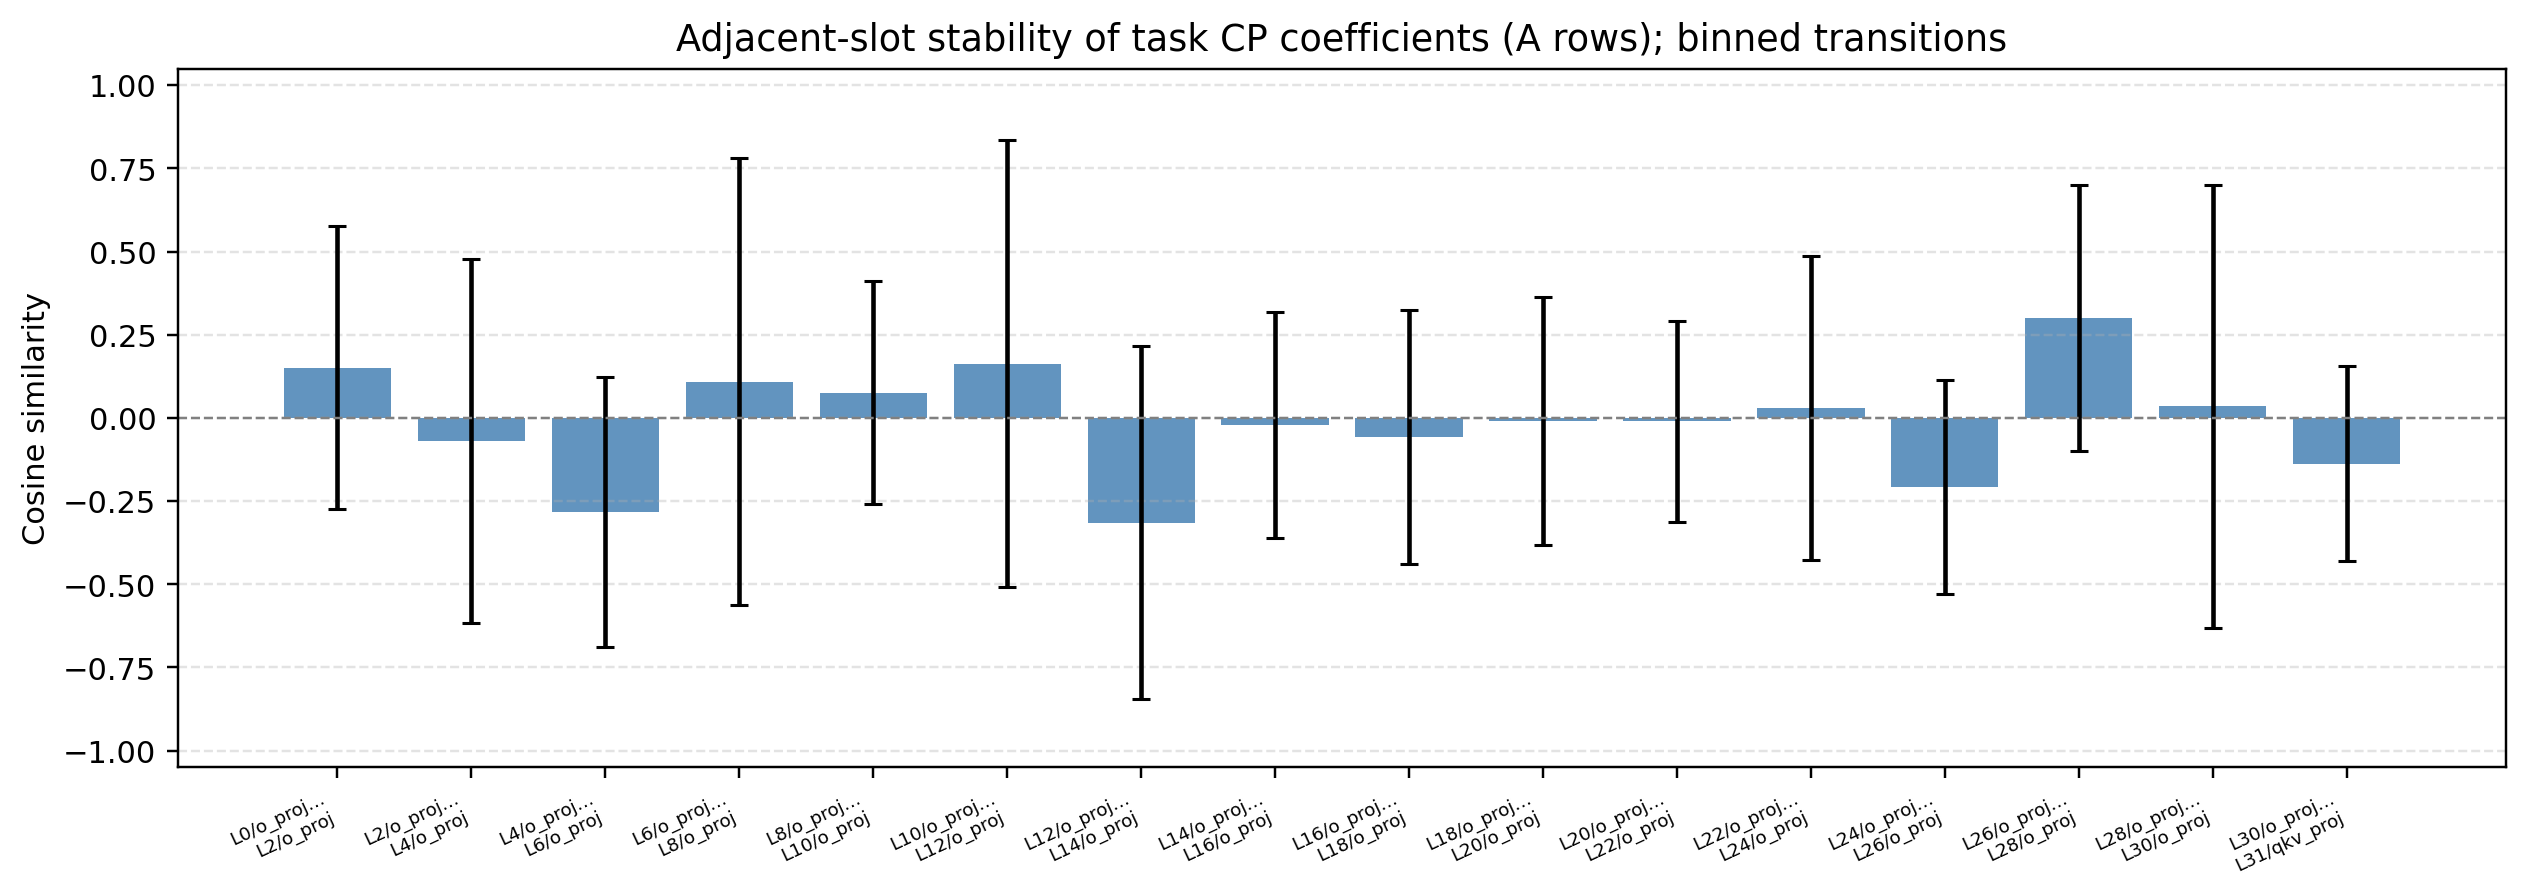
\includegraphics[width=\linewidth]{fig/cpmergeafter_cross_layer_task_A_adjacent_cosine.png}
    \caption{Adjacent-slot stability of task CP coefficients (A rows).}
    \label{fig:adjacent_cross_layer}
\end{figure}

For each task, Figure~\ref{fig:adjacent_cross_layer} reports the cosine similarity between its row of $A$ in one slot and in the next processed slot, as mean $\pm$ std over tasks. Several transitions show positive mean alignment, for example 0.535 from \texttt{o\_proj} to \texttt{qkv\_proj} in layer 10 and 0.454 from \texttt{qkv\_proj} in layer 27 to \texttt{o\_proj} in layer 28. Other transitions are near zero or negative, with standard deviations often between 0.3 and 0.9. Two factors explain this variation. \texttt{o\_proj} and \texttt{qkv\_proj} are different operators with different geometry, and CP factors are identifiable only up to scaling, sign, and permutation, so $A$ need not be stable across independently fitted layers. We therefore read this plot as a continuity check for layer-wise fitting, not as evidence of a single task embedding shared across all depths.


\begin{figure}[h]
    \centering
    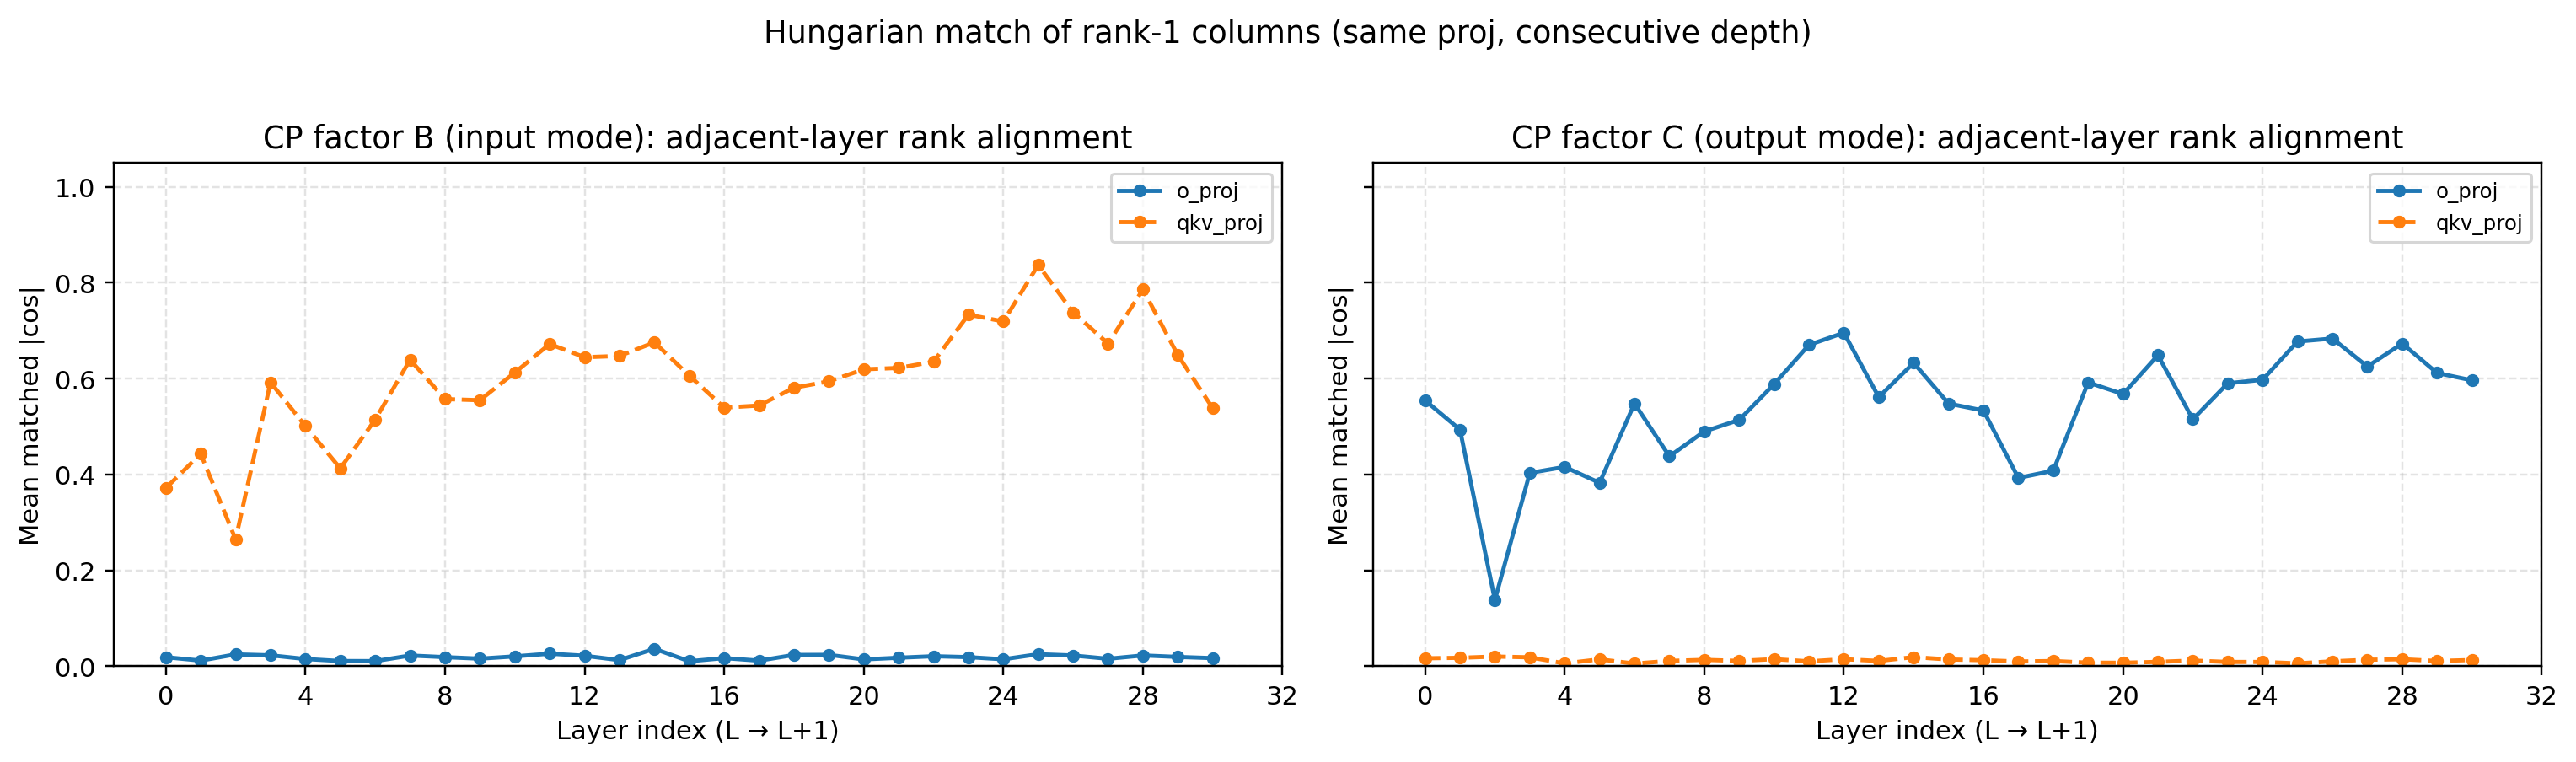
\includegraphics[width=\linewidth]{fig/cpmergeafter_cross_layer_BC_rank_alignment_adjacent.png}
    \caption{Alignment of rank-one components across depth. $|\cos|$ is the absolute cosine similarity between matched L2-normalized columns of the CP factor matrices $B$ or $C$ in adjacent layers.}
    \label{fig:bc_bank}
\end{figure}

Because the order of CP components within a layer is arbitrary, we match the normalized factor columns of consecutive layers with the Hungarian algorithm, separately for \texttt{o\_proj} and \texttt{qkv\_proj}. Figure~\ref{fig:bc_bank} shows that the results differ by factor and projection. For $B$ on \texttt{qkv\_proj}, the matched $|\cos|$ between adjacent layers is moderate to high, often between 0.37 and 0.84 with a peak of about 0.84 from layer 25 to layer 26, which suggests recurring rank-one input directions along depth for QKV adapters. For $B$ on \texttt{o\_proj}, the matched $|\cos|$ is much lower, often between 0.01 and 0.04, so the components of output projections are not stable across independently decomposed layers, as expected from the identifiability limits of CP decomposition. For $C$, \texttt{o\_proj} shows higher matched similarity than \texttt{qkv\_proj}, with many \texttt{o\_proj} pairs between 0.4 and 0.7 and \texttt{qkv\_proj} pairs often between 0.006 and 0.02. Whether a rank-one component keeps its meaning across depth must therefore be assessed separately for each factor and projection type.
    

    \subsection{Clusterized LoRA Library (C-LoRA)}
    \label{sec:clora}

    \citet{ostapenko2024towards} show that grouping tasks by LoRA similarity leads to positive transfer. Their clustering requires the \textit{task ID} of every example and a trained adapter for every task before clustering. We instead cluster at the text level, which needs neither and achieves competitive results. Figure~\ref{fig:cluster_performance}(c) visualizes the embeddings of 100 examples per cluster; similar texts fall into the same clusters.

    To reduce task conflicts at the \textit{text level}, we train each \textit{expert}
    on a group of similar tasks obtained by clustering the instructions, without
    manual intervention. Each adapter then specializes in a subset of data with
    similar characteristics, which can reduce interference within its training data. Formally,
    let $E(\cdot)$ denote a pretrained sentence encoder. For each data sample,
    the sentence representation of an instruction $I_{i}$ is computed as
    $e_{i}=E(I_{i})$. We then apply the k-means algorithm to cluster all instruction
    embeddings $\{e_{i}\}$ in the training dataset into $K$ clusters. We train
    each LoRA adapter based on the instructions from each cluster. For each pre-trained
    weight $W_{0}$, we obtain corresponding LoRA adapters
    $\{B_{1}A_{1},\ldots,B_{K}A_{K}\}$.
    \subsubsection{Effect of the number of clusters}
    \label{sec:clustering}

    \begin{figure}[h]
        \centering
        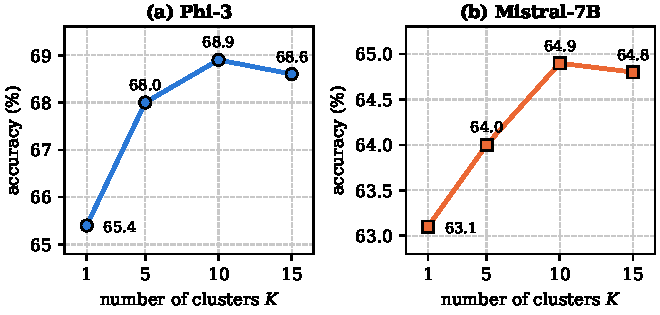
\includegraphics[width=0.64\textwidth]{fig/cluster_acc.pdf}\hfill
        \begin{minipage}[b]{0.33\textwidth}
            \centering
            {\small\textbf{(c) Instruction embeddings}}\\[2pt]
            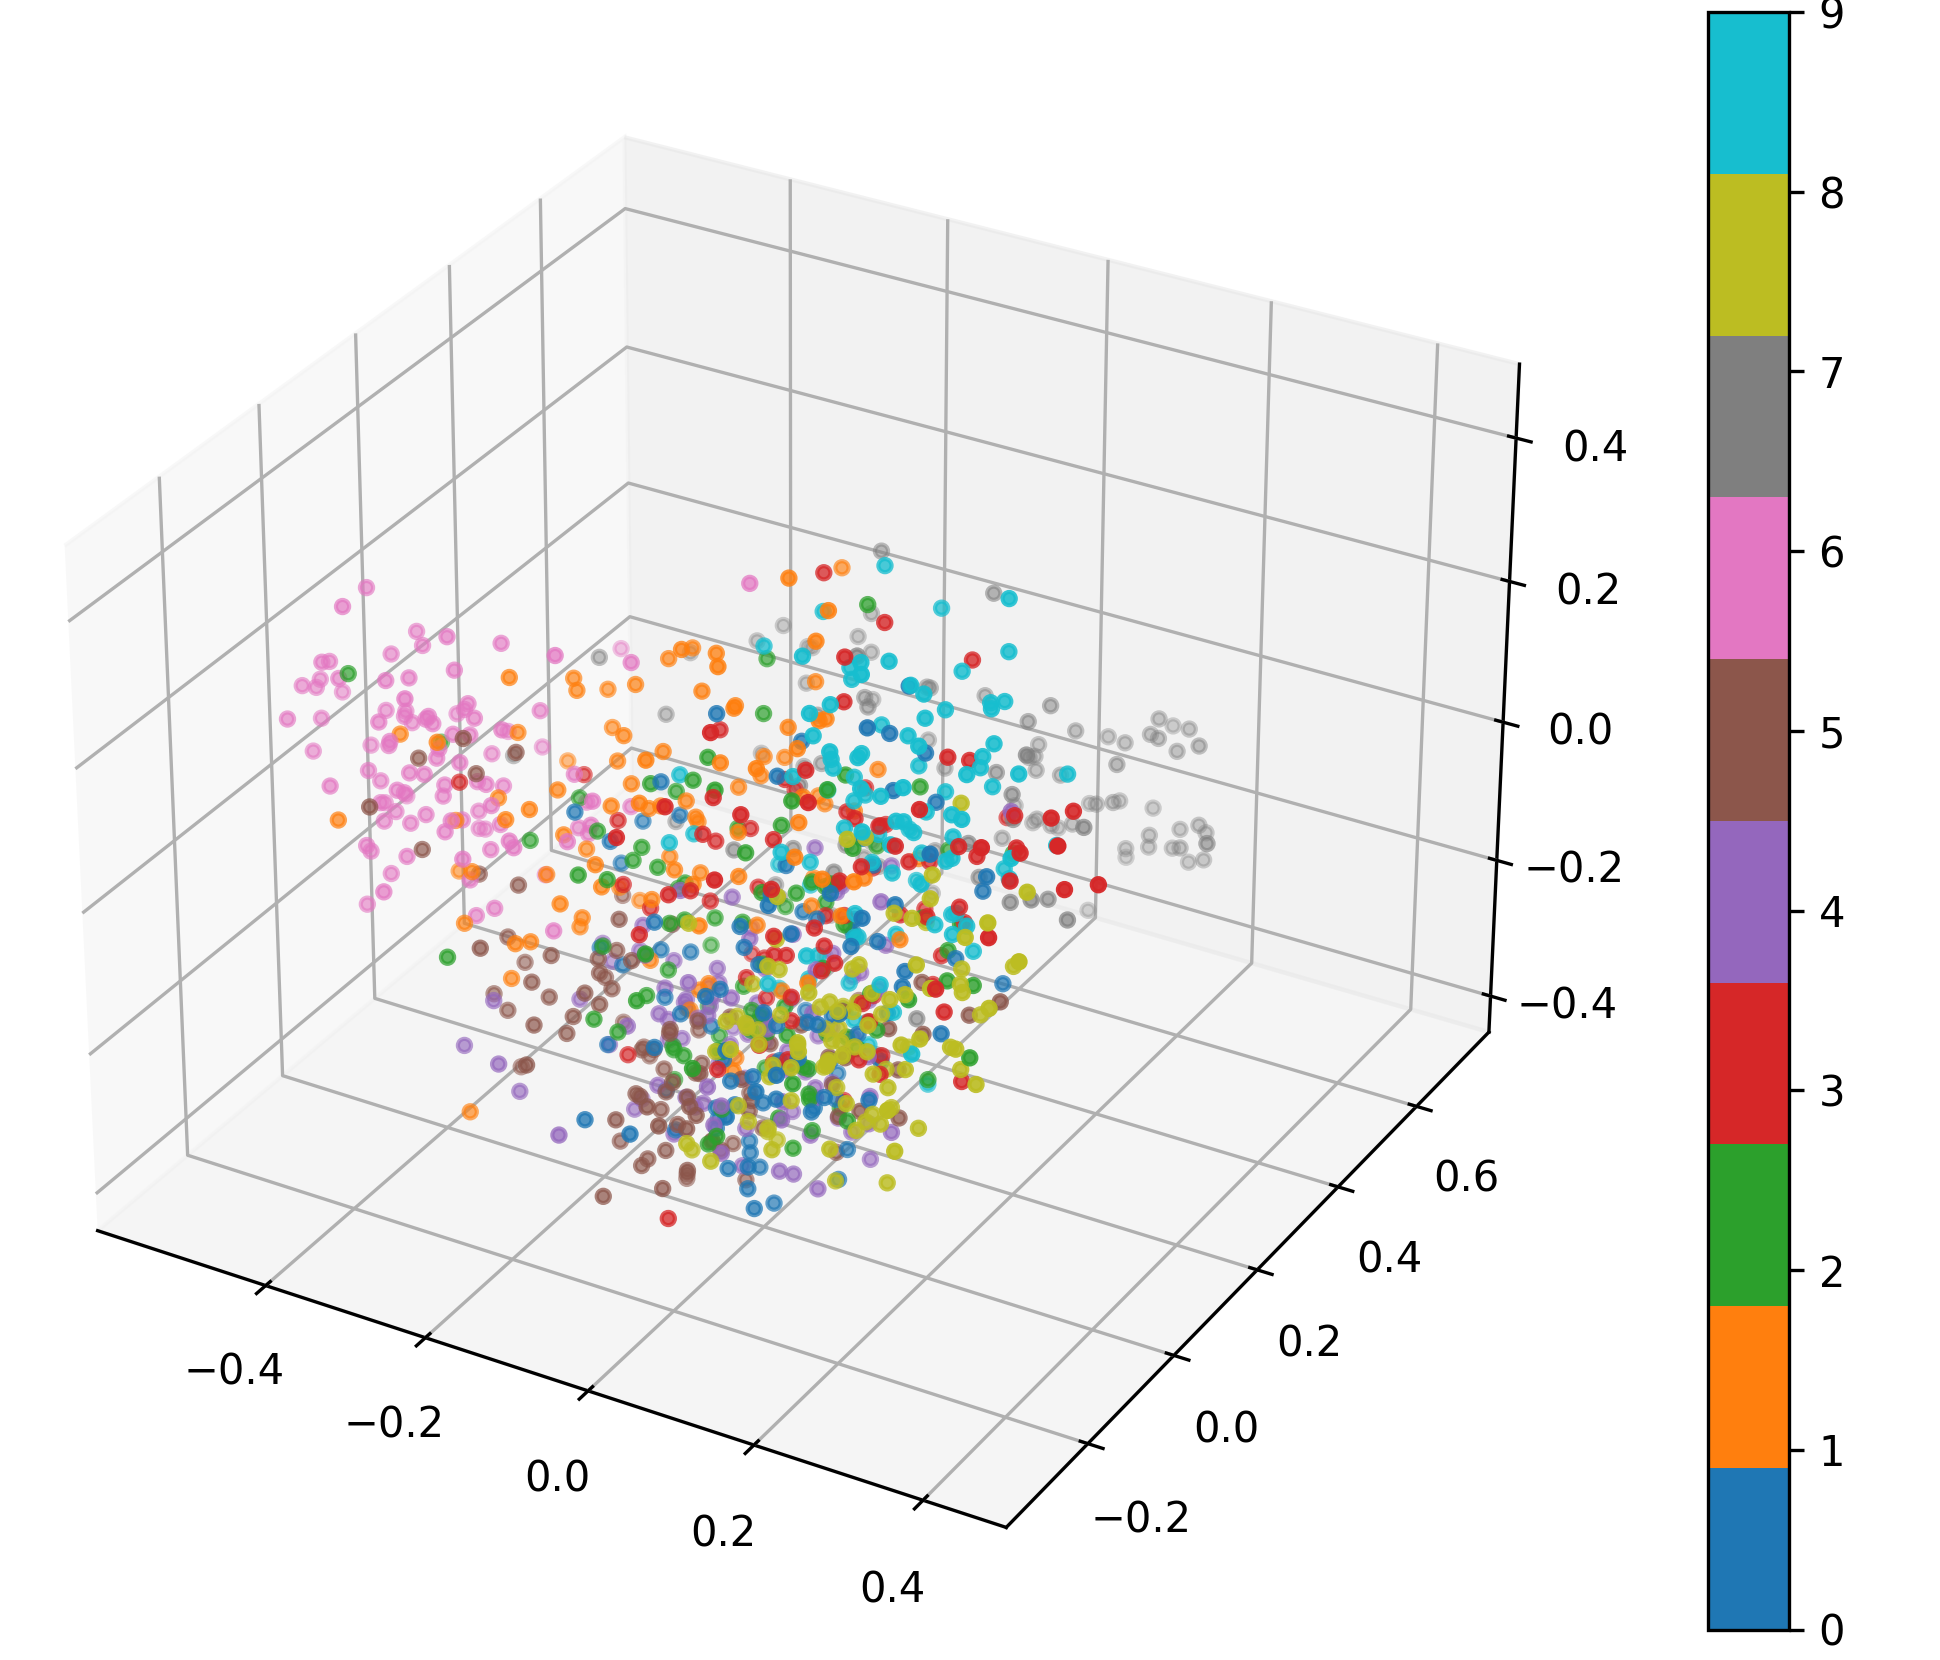
\includegraphics[width=\linewidth]{fig/embedding_3d.png}
        \end{minipage}
        \caption{Effect of the number of clusters $K$ on zero-shot accuracy with (a) Phi-3 and (b) Mistral-7B. (c) Sentence embeddings of 100 instructions per cluster, colored by cluster ($K=10$).}
        \label{fig:cluster_performance}
    \end{figure}

    Figure~\ref{fig:cluster_performance} shows accuracy as a function of the
    number of clusters for Phi-3 (a) and Mistral-7B (b). With Phi-3,
    accuracy increases from about 65.4\% with 1 cluster to 68.9\% with 10
    clusters and stays at this level up to 15 clusters. With Mistral-7B, accuracy
    rises more gradually, from 63.1\% with 1 cluster to 64.9\% with 10 clusters.
    Choosing the number of clusters automatically remains an open question.


\subsection{Zero-shot Results on Mistral 7B}
\label{sec:zero_shot_mistral}

Table~\ref{tab:zeroshot_mistral} reports zero-shot results with Mistral-7B. Unlike on Phi-3, the multi-task adapter improves over the base model, from 59.5\% to 63.1\%. With the C-LoRA library, CP merging obtains the highest average accuracy (65.0\%), followed by uniform merging (64.9\%).
\begin{table*}[ht]
\small
\centering
\begin{adjustbox}
{width=1.0\textwidth}
\begin{tabular}{l|cccccccccc|c} 
\Xhline{1.6pt}
\multicolumn{1}{c|}{} & \multicolumn{3}{c}{\textbf{Common Sense}} & \multicolumn{4}{c}{\textbf{Question Answering}} & \multicolumn{2}{c}{\textbf{Coding}} & \multicolumn{1}{c}{\textbf{ Reasoning}} & \multicolumn{1}{c}{\textbf{AVG}} \\
\cmidrule(lr){2-4}  \cmidrule(lr){5-8} \cmidrule(lr){9-10}
\cmidrule(lr){11-11}
\multicolumn{1}{c|}{} & \textbf{Piqa} & \textbf{Wg} & \textbf{Hswag} & \textbf{Boolq} & \textbf{Obqa} & \textbf{ArcE} & \textbf{ArcC} & \textbf{HE} & \textbf{Mbpp} & \textbf{BBH} & \multicolumn{1}{c}{\textbf{AVG}} \\
\midrule

\rowcolor{lightgray}\multicolumn{12}{c}{\textbf{Mistral (7B) with LoRA library}  } \\
\textbf{BASE}  & 81.1  & 66.5  & 78.8  & 82.2 & 44.6 & 68.9 & 49.6 & 28.0 & 47.5 & 47.9 & \cellcolor[HTML]{FDE9E8}59.5\\ 
\textbf{Multi-task}  & 81.9 & 68.6 & 79.5 & 84.6 & \textbf{50.4} & 84.8 & 60.0 & 24.4 & 47.5 & 49.2 & \cellcolor[HTML]{FDE9E8}63.1 \\

\textbf{Uniform}& 82.1 & 67.2 & 79.6 & 82.7 & 45.2 & 78.7 & 54.8 & 29.9 & 49.4 & 49.0 &  \cellcolor[HTML]{FDE9E8}61.9 \\

\textbf{Ties-merging} & 82.4 & 70.6 & 79.9 & 87.6 & 44.2 & 81.1 & 57.3 & \textbf{31.7} & 47.9 & 46.2 & \cellcolor[HTML]{FDE9E8}62.9 \\
\textbf{Task Arithmetic} & 82.3 & 67.1 & 79.5 & 82.4 & 45.3 & 78.4 & 54.8 & 30.0 & 49.4 & 49.1 &  \cellcolor[HTML]{FDE9E8}61.8\\
\textbf{Ties w/DARE} & 82.3 & 70.3 & 79.8 & 87.4 & 44.3 & 81.3 & 57.2 & 31.6 & 47.6 & 46.3 & \cellcolor[HTML]{FDE9E8}62.8\\
\textbf{TA w/DARE} & 82.2 & 67.3 & 79.5 & 82.2 & 45.4 & 78.3 & 54.9 & 30.1 & 49.5 & 49.2 & \cellcolor[HTML]{FDE9E8}61.9\\
\textbf{TSV merging} & 81.6 & 70.3 & 78.9 & 82.8 & 42.8 & 84.0 & 58.3 & 28.7 & 49.7 & 49.5 & 62.7\cellcolor[HTML]{FDE9E8}\\

\midrule
\rowcolor{lightgray}\multicolumn{12}{c}{\textbf{Mistral (7B) with C-LoRA library }} \\
\textbf{Uniform}  & 82.4  & 71.4 & 81.2 & 87.6 & 49.2 & 86.0 & 60.5  & 29.3 & 50.0 & 50.0 & \cellcolor[HTML]{FDE9E8}64.9 \textcolor{red}{\scriptsize ↑2.2} \\ 
\textbf{CP-merging} & \textbf{82.6} & \textbf{71.7} & \textbf{81.6} & \textbf{87.8} & 49.3  & \textbf{86.0} & \textbf{60.6} & 29.3  & \textbf{50.2}  & \textbf{50.7} & \cellcolor[HTML]{FDE9E8}\textbf{65.0} \textcolor{red}{\scriptsize ↑2.3} \\ \hline

\Xhline{1.6pt}
\end{tabular}
\end{adjustbox}
\caption{Zero-shot accuracy on 10 downstream benchmarks with Mistral-7B.}
\label{tab:zeroshot_mistral}
\end{table*}

\end{document}
